\documentclass[11pt, oneside]{report}

\usepackage{config/style}
\usepackage{config/code}
\usepackage{amsmath}
\usepackage{csquotes}
\usepackage{tikz}
\usepackage{array}
\usepackage{caption}
\usetikzlibrary{matrix,calc,shapes.misc,fit, decorations.pathreplacing, positioning, arrows.meta, fit, backgrounds}
\addbibresource{references.bib}

\begin{document}
\newcommand{\paperauthor}{Eric Seidel, Malte Gaelings, Paul Sandow, Mikel Lautsch, Mario Zinta}
\newcommand{\papersupervisor}{Prof. Dr. Frau Anderle}
\newcommand{\paperuniversity}{Westfälische hochschule}

\newcommand{\papertitle}{Stochastik und Lineare Algebra Übungsaufgaben}
\newcommand{\papermajorheading}{Informatik}
\newcommand{\paperminorheading}{SLA}

	\begin{titlepage}

\newcommand{\HRule}{\rule{\linewidth}{0.5mm}} % Defines a new command for the horizontal lines, change thickness here

\center % Center everything on the page

%----------------------------------------------------------------------------------------
%	HEADING SECTIONS
%----------------------------------------------------------------------------------------

\textsc{\LARGE \paperuniversity}\\[1.0cm] % Name of your university/college
\textsc{\Large \papermajorheading}\\[0.2cm] % Major heading such as course name
\textsc{\large \paperminorheading}\\[0.75cm] % Minor heading such as course title

%----------------------------------------------------------------------------------------
%	TITLE SECTION
%----------------------------------------------------------------------------------------

\HRule \\[0.4cm]
{ \huge \bfseries \papertitle}\\[0.05cm] % Title of your document
\HRule \\[3.5cm]

\begin{center}
	\makebox[0.8\textwidth]{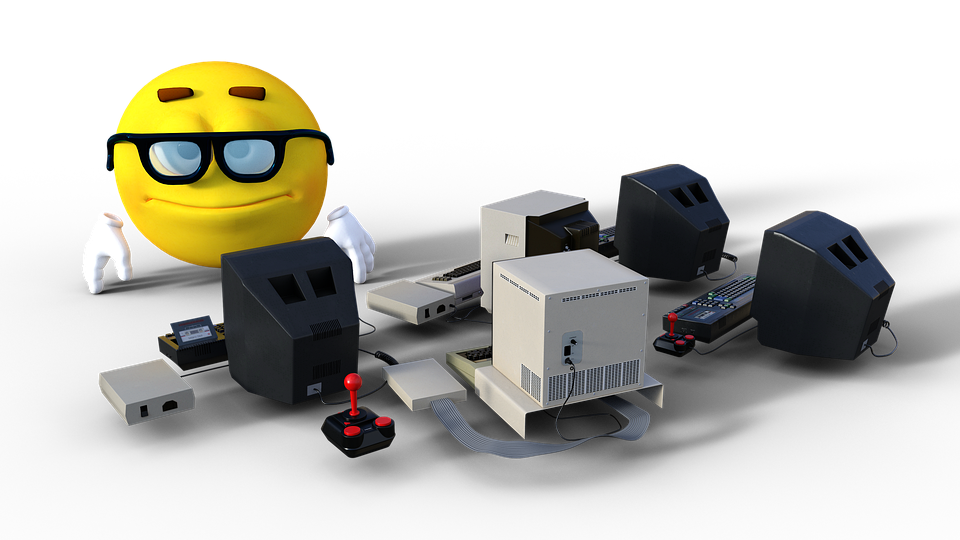
\includegraphics[width=0.8\textwidth]{frontpage.png}}
\end{center}

\vfill % Fill the rest of the page with whitespace

%----------------------------------------------------------------------------------------
%	AUTHOR SECTION
%----------------------------------------------------------------------------------------

\begin{minipage}{0.4\textwidth}
	\begin{flushleft} \large
	\emph{Author(s):}\\
	\paperauthor
	\end{flushleft}
	\end{minipage}
	~
	\begin{minipage}{0.4\textwidth}
	\begin{flushright} \large
	\emph{Supervisor(s):} \\
	\papersupervisor
	\end{flushright}
\end{minipage}\\[1cm]

%----------------------------------------------------------------------------------------
%	DATE SECTION
%----------------------------------------------------------------------------------------

{\large \today}\\ % Date, change the \today to a set date if you want to be precise

\end{titlepage}


	\clearpage

	\thispagestyle{empty}
	\pagenumbering{gobble}

	\renewcommand{\abstractname}{Copyright \textcopyright \xspace \the\year \xspace \paperuniversity}

\begin{abstract}
\begin{center}

This document, including appendices, is property of \paperuniversity \xspace and is confidential, privileged and only for use of the intended addressees and may not be used, published or redistributed without the prior written consent of \paperuniversity \xspace.

\end{center}
\end{abstract}

	\renewcommand{\abstractname}{Einleitung}
\begin{abstract}

Die vorliegende Aufgabensammlung wurde von Frau Prof. Dr. Anderle dankenswerterweise 
zur Verfügung gestellt. Sie dient der Vertiefung und Anwendung der 
Inhalte der Vorlesung \textit{Stochastik und Lineare Algebra}.

Die Aufgaben decken alle für die Klausur 2025 relevanten Themen ab und sollen Ihnen die 
Möglichkeit geben, Ihr Verständnis zu festigen und sich gezielt auf die Prüfung vorzubereiten.

Obwohl die Aufgaben mit Sorgfalt ausgewählt und aufbereitet wurden, kann \textbf{für die vollständige 
Richtigkeit und Fehlerfreiheit keine Gewähr übernommen werden}. Wir empfehlen, die Lösungswege 
kritisch zu reflektieren und bei Unklarheiten Rücksprache zu halten.

Diese Aufgabensammlung dient als Hilfestellung. Sie sollten versuchen, die Aufgaben 
selbstständig und nur mit den erlaubten Hilfsmitteln zu bearbeiten und erst nach 
deren Bearbeitung Ihren eigenen Lösungsweg mit den hier 
vorliegenden Lösungsvorschlägen zu überprüfen.

Diese Aufgabensammlung enthält auch Lösungen zu den Bonustests. Da diese Tests teilweise viele Variationen 
aufweisen, ist es wahrscheinlich, dass Ihre konkreten Zahlenwerte und Ihr Ergebnis von den hier 
dargestellten abweichen werden. Beachten Sie des Weiteren, dass auch die Reihenfolge der Bonustests variieren kann. 
Achten Sie deswegen bitte auf den Titel des je\-weiligen Tests, um die korrekte Lösung zuzuordnen.

Die hier vorgestellten Rechenwege sind der Verständlichkeit halber bewusst sehr detailliert gehalten. 
In der Prüfung sollten Sie aus zeitlichen Gründen eine kompaktere Darstellung wählen. 
Es empfiehlt sich, Ihren Professor oder Ihre Professorin mit einer Ihrer Beispielrechnungen zu konsultieren. 
So können Sie sicherstellen, dass Ihre Notation korrekt ist, keine wesentlichen Schritte fehlen und Ihre Ausführungen 
den Anforderungen entsprechen, ohne unnötig ausführlich zu sein.

Haben Sie des Weiteren keine Bedenken, einen anderen Lösungsweg zu verfolgen. Die hier 
aufgezeigten Lösungswege sind lediglich Vorschläge und sind keineswegs die einzig korrekten Wege.

Wir wünschen Ihnen viel Erfolg bei der Bearbeitung und eine gute Klausurvorbereitung!

\end{abstract}

	\tableofcontents

	\clearpage

	\pagenumbering{arabic}

	\part{Semesterzusammenfassung}
	\chapter{Vektoren}

\section{Definition eines Vektors}

Sollen nicht nur einzelne Zahlen festgehalten werden, sondern mehrere Zahlen,
die in einer bestimmten Reihenfolge zusammengehören, kommen Vektoren ins Spiel.

Ein \textbf{Vektor} im $\mathbb{R}^n$ ist formal betrachtet ein Element des
mathematischen Raumes $\mathbb{R}^n$. Das bedeutet, ein Vektor ist ein
geordnetes n-Tupel reeller Zahlen. Ein solcher Vektor wird oft als Spalte
geschrieben:

\[
    \vec{v} = \begin{pmatrix}
        v_1 \\ v_2 \\ \vdots \\ v_n
    \end{pmatrix}
\]

wobei $v1, v2, \dots, v_n$ reelle Zahlen sind, die sogenannten
\textbf{Komponenten} oder \textbf{Koordinaten} des Vektors. Die Zahl n gibt die
\textbf{Dimension} des Vektors an.

\begin{itemize}
    \item Für n=2 liegen Vektoren in der Ebene ($\mathbb{R}^2$) vor, z.B. $\begin{pmatrix}
                  1 \\ 2
              \end{pmatrix}$.
    \item Für n=3 liegen Vektoren im Raum ($\mathbb{R}^3$) vor, z.B. $\begin{pmatrix}
                  1 \\ 2 \\ 3
              \end{pmatrix}$.
    \item Für $n > 3$ wird von höherdimensionalen Räumen gesprochen, die schwerer
          vorstellbar, aber mathematisch ebenso bedeutsam sind.
\end{itemize}

Vektoren werden normalerweise mit einem Pfeil gekennzeichnet $\vec{v}$, jedoch
wird der einfachkeit halber oft darauf verzichtet.

Ein Vektor (zumindest in $\mathbb{R}^2$ und $\mathbb{R}^3$) kann als ein
\textbf{Pfeil} interpretiert werden, der von einem Punkt zu einem anderen
zeigt. Dieser Pfeil hat eine bestimmte \textbf{Länge} (Betrag) und eine
bestimmte \textbf{Richtung}. Wichtig ist, dass Vektoren oft als "frei"
betrachtet werden, d.h., ein Pfeil repräsentiert denselben Vektor, egal wo sein
Anfangspunkt im Raum liegt, solange Länge und Richtung gleich bleiben. Häufig
wird der Pfeil im Ursprung des Koordinatensystems begonnen; dann zeigen seine
Koordinaten direkt auf den Endpunkt des Pfeils.

Mit Vektoren können zwei grundlegende Rechenoperationen durchgeführt werden:
%
\begin{enumerate}
    \item \textbf{Vektoraddition:} Zwei Vektoren derselben Dimension n können addiert werden, indem ihre entsprechenden Komponenten addiert werden. Wenn $\vec{u} = \begin{pmatrix}
                  u_1 \\ u_2 \\ \vdots \\ u_n
              \end{pmatrix}$ und $v = \begin{pmatrix}
                  v_1 \\ v_2 \\ \vdots \\ v_n
              \end{pmatrix}$, dann ist ihre Summe:
          \[
              u + v = \begin{pmatrix}
                  u_1 + v_1 \\ u_2 + v_2 \\ \vdots \\ u_n + v_n
              \end{pmatrix}
          \]
          Geometrisch entspricht die Addition von Vektoren dem Aneinanderhängen der
          Pfeile (Parallelogrammregel oder Spitze-an-Schaft-Regel).

    \item \textbf{Skalare Multiplikation:} Ein Vektor kann mit einer reellen Zahl (einem sogenannten \textbf{Skalar}) multipliziert werden. Dabei wird jede Komponente des Vektors mit diesem Skalar multipliziert. Wenn $c \in \mathbb{R}$ ein Skalar ist und $\vec{v} = \begin{pmatrix} v_1 \\ v_2 \\ \vdots \\ v_n \end{pmatrix}$ ein Vektor, dann ist das Produkt:

          \[
              c \cdot \vec{v} = \begin{pmatrix} c \cdot v_1 \\ c \cdot v_2 \\ \vdots \\ c \cdot v_n \end{pmatrix}
          \]

          Geometrisch bewirkt die skalare Multiplikation eine Streckung oder Stauchung
          des Vektors. Wenn der Skalar negativ ist, kehrt sich zusätzlich die Richtung
          des Vektors um.

\end{enumerate}

Diese beiden Operationen sind fundamental und bilden die Grundlage für die
Struktur eines \textbf{Vektorraums}, ein zentrales Konzept in der linearen
Algebra. Ein Vektor ist also nicht nur ein Tupel von Zahlen, sondern ein
Objekt, das sich auf definierte Weise mit anderen Vektoren (Addition) und
Skalaren (skalare Multiplikation) kombinieren lässt.

\section{Parallelität}

Zwei Vektoren sind Parallel zueinander, falls ein Vektor ein vielfaches eines
anderen ist. Um zu prüfen, ob zwei Vektoren $\vec{a}, \vec{b}$ parallel
zueinander sind, können einfach die einzelnen Einträde dividiert werden. Wenn
alle Ergebnisse gleich sind, sind die Vektoren Parallel.
	\chapter{Vektorraum}

\section{Definition}

Ein Vektorraum über einem Körper $\mathbb{K}$ (Hier inden Vorlesungen immer
$\mathbb{R}$) ist eine Menge $V$, deren Elemente Vektoren genannt werden,
zusammen mit zwei Operationen:
\begin{itemize}
    \item der Vektoraddition $+ : V \times V \to V$, $(v, w) \mapsto v+w$,
    \item der Skalarmultiplikation $\cdot : \mathbb{K} \times V \to V$, $(s, v) \mapsto s
              \cdot v$.
\end{itemize}

Damit $(V, +, \cdot)$ als Vektorraum über $\mathbb{K}$ bezeichnet werden kann,
müssen die folgenden Axiome für alle Vektoren $u, v, w \in V$ und alle Skalare
$s, t \in \mathbb{K}$ erfüllt sein:

\textbf{Axiome der Vektoraddition} (d.h. $(V,+)$ ist eine abelsche Gruppe):
\begin{itemize}
    \item $v + w = w + v$ (Kommutativgesetz der Addition)
    \item $u + (v + w) = (u + v) + w$ (Assoziativgesetz der Addition)
    \item Es existiert ein Nullelement $\vec{0} \in V$, sodass für alle $v \in V$ gilt:
          $\vec{0} + v = v$ (Existenz des neutralen Elements der Addition)
    \item Zu jedem $v \in V$ existiert ein inverses Element $-v \in V$, sodass gilt: $v +
              (-v) = \vec{0}$ (Existenz des inversen Elements der Addition)
\end{itemize}

\textbf{Axiome der Skalarmultiplikation} (und Kompatibilität mit der Vektoraddition):
\begin{itemize}
    \item $s \cdot (v + w) = s \cdot v + s \cdot w$ (Distributivgesetz bezüglich der Vektoraddition)
    \item $(s + t) \cdot v = s \cdot v + t \cdot v$ (Distributivgesetz bezüglich der Skalaraddition)
    \item $(s \cdot t) \cdot v = s \cdot (t \cdot v)$ (Assoziativgesetz der Skalarmultiplikation)
    \item $1 \cdot v = v$, wobei $1$ das Einselement des Körpers $\mathbb{K}$ ist (Neutralität des Einselements des Körpers)
\end{itemize}

\paragraph{Erläuterung}
Die Vektorraumaxiome stellen sicher, dass die Addition von Vektoren und die
Multiplikation von Vektoren mit Skalaren sich in einer Weise verhalten, die
konsistent und "vernünftig" ist. Die ersten vier Axiome definieren die
Eigenschaften der Vektoraddition (die Vektoren bilden eine abelsche Gruppe),
während die übrigen Axiome die Wechselwirkung mit der Skalarmultiplikation
regeln. Obwohl die Liste der Axiome zunächst umfangreich erscheinen mag, fassen
sie im Kern zusammen, dass sich das Rechnen mit Vektoren und Skalaren in
vielerlei Hinsicht analog zum Rechnen mit "normalen" Zahlen (wie den reellen
Zahlen $\mathbb{R}$) und deren bekannten Rechengesetzen verhält. Es sind also
genau die Eigenschaften, die man intuitiv von Operationen erwarten würde, die
man "Addition" und "skalare Multiplikation" nennt.

	\chapter{Lineare Abbildungen}

Lineare Abbildungen sind ein fundamentales Konzept in der Mathematik, besonders in der linearen Algebra. Sie beschreiben auf eine sehr spezielle Weise, wie ein Vektor (oder eine Zahl) in einen anderen transformiert wird.

\section{Was ist überhaupt eine lineare Abbildung? (Der einfache Fall)}

\textit{Eine Lineare Abbildung ist eine Abbildung mit Konstanten Anteil 0.}

Das bedeutet, wenn man sich den Graphen der Funktion vorstellt, muss er \textbf{immer durch den Ursprung gehen} (also durch den Punkt $(0,0)$).

\textbf{Beispiele:}
\begin{itemize}
    \item $f(x) = 3x$
    \begin{itemize}
        \item Hier wird jede Zahl $x$ einfach mit 3 multipliziert.
        \item Wenn $x=0$ eingesetzt wird, kommt $f(0) = 3 \cdot 0 = 0$ raus. Der konstante Anteil ist 0.
        \item Grafisch ist das eine Gerade, die durch den Ursprung geht.
        \item \textbf{Das ist eine lineare Abbildung.}
    \end{itemize}

    \item $f(x) = 3x + 3$
    \begin{itemize}
        \item Hier wird $x$ mit 3 multipliziert, und dann wird noch 3 addiert.
        \item Wenn $x=0$ eingesetzt wird, kommt $f(0) = 3 \cdot 0 + 3 = 3$ raus.
        \item Dieser "$+3$"-Teil ist der "konstante Anteil", der eben nicht Null ist.
        \item Grafisch ist das eine Gerade, die die y-Achse bei 3 schneidet, nicht im Ursprung.
        \item \textbf{Das ist KEINE lineare Abbildung.}
    \end{itemize}
\end{itemize}

\section{Lineare Abbildungen zwischen zwei Vektorräumen}

Nun wird es etwas allgemeiner. Man stelle sich vor, man hat nicht nur einzelne Zahlen, sondern ganze Räume voller Vektoren. Eine lineare Abbildung kann nun Vektoren aus einem Vektorraum in Vektoren eines anderen Vektorraums überführen. Damit das "linear" im Sinne der linearen Algebra ist, müssen zwei ganz wichtige Eigenschaften erfüllt sein: \textbf{Additivität} und \textbf{Homogenität}.

\subsection{Homogenität ("Skalierungstreue")}

Die Homogenität besagt:
$$f(\lambda \cdot v) = \lambda \cdot f(v)$$

Bedeutung:
\begin{itemize}
    \item $\lambda$ (Lambda) ist ein Skalar.
    \item $v$ ist ein Vektor.
    \item $\lambda \cdot v$ bedeutet: Man nimmt den Vektor $v$ und streckt oder staucht ihn um den Faktor $\lambda$.
    \item $f(v)$ ist das Ergebnis, wenn die Abbildung $f$ auf den Vektor $v$ angewendet wird.
\end{itemize}
Die Regel besagt: Es ist egal, ob ein Vektor \textbf{zuerst skaliert} und \textbf{dann die Abbildung angewendet wird}, ODER ob \textbf{zuerst die Abbildung auf den Vektor angewendet wird} und \textbf{das Ergebnis dann skaliert wird}. Es muss dasselbe Ergebnis resultieren.

\textbf{Beispiel $f(x) = 3x$ (hier ist $x$ ein eindimensionaler Vektor):}

Sei $\lambda = 2$ und der "Vektor" $x=2$.
\begin{itemize}
    \item \textbf{Linke Seite der Gleichung: $f(\lambda \cdot x)$}
    \begin{enumerate}
        \item Zuerst skalieren: $\lambda \cdot x = 2 \cdot 2 = 4$.
        \item Dann $f$ anwenden: $f(4) = 3 \cdot 4 = 12$.
    \end{enumerate}
    \item \textbf{Rechte Seite der Gleichung: $\lambda \cdot f(x)$}
    \begin{enumerate}
        \item Zuerst $f$ anwenden: $f(x) = f(2) = 3 \cdot 2 = 6$.
        \item Dann das Ergebnis skalieren: $\lambda \cdot f(2) = 2 \cdot 6 = 12$.
    \end{enumerate}
\end{itemize}
Es gilt $12 = 12$. Die Homogenität ist erfüllt.

\textit{Der Ausdruck $f(4) = 3 \cdot 4 = 2 \cdot f(2) = f(2 \cdot 2)$ zeigt genau das:}
\begin{itemize}
    \item $f(2 \cdot 2)$ ist die linke Seite (erst skalieren, dann abbilden).
    \item $2 \cdot f(2)$ ist die rechte Seite (erst abbilden, dann skalieren).
\end{itemize}

\subsection{Additivität ("Summentreue")}

Die Additivität besagt:
$$f(v + w) = f(v) + f(w)$$

Bedeutung:
\begin{itemize}
    \item $v$ und $w$ sind zwei Vektoren (aus demselben Vektorraum).
    \item $v+w$ ist die Summe der beiden Vektoren.
\end{itemize}
Die Regel besagt: Es ist egal, ob zwei Vektoren \textbf{zuerst addiert} und \textbf{dann die Abbildung auf die Summe angewendet wird}, ODER ob \textbf{zuerst die Abbildung auf jeden Vektor einzeln angewendet wird} und \textbf{dann die Ergebnisse addiert werden}. Es muss dasselbe Ergebnis resultieren.

\textbf{Beispiel mit $f(x) = 3x$:}

Seien $v=1$ und $w=5$.
\begin{itemize}
    \item \textbf{Linke Seite der Gleichung: $f(v+w)$}
    \begin{enumerate}
        \item Zuerst addieren: $v+w = 1+5 = 6$.
        \item Dann $f$ anwenden: $f(6) = 3 \cdot 6 = 18$.
    \end{enumerate}
    \item \textbf{Rechte Seite der Gleichung: $f(v) + f(w)$}
    \begin{enumerate}
        \item $f$ auf $v$ anwenden: $f(v) = f(1) = 3 \cdot 1 = 3$.
        \item $f$ auf $w$ anwenden: $f(w) = f(5) = 3 \cdot 5 = 15$.
        \item Die Ergebnisse addieren: $3 + 15 = 18$.
    \end{enumerate}
\end{itemize}
Es gilt $18 = 18$. Die Additivität ist erfüllt.

\textbf{Zusammenfassend für Vektorräume:}
Eine Abbildung $f$ zwischen zwei Vektorräumen ist linear, wenn sie
\begin{enumerate}
    \item \textbf{homogen} ist: $f(\lambda \cdot v) = \lambda \cdot f(v)$
    \item \textbf{additiv} ist: $f(v + w) = f(v) + f(w)$
\end{enumerate}
Diese beiden Bedingungen sind der Kern dessen, was eine lineare Abbildung ausmacht. Sie sorgen dafür, dass die Struktur des Vektorraums durch die Abbildung "respektiert" wird.

\textbf{Warum ist das wichtig?}
Lineare Abbildungen sind grundlegend für viele Transformationen und haben Eigenschaften, die in Bereichen wie Computergrafik, Physik und Ingenieurwesen nützlich sind.
	\chapter{Linearkombinationen}

Eine Linearkombination beschreibt eine Summe aus Vektoren. Das Ergebnis aus einer Linearkombination von Vektoren ist selbst ein Vektor. Ein Vektor ist eine Linearkombinationen von Vektoren, wenn es $a, b \in \mathbb{R}$ gibt, sodass $u = a \cdot v + b \cdot w$ gilt. Dies berechnet man durch ein Lineares Gleichungssystem

\section{Beispiel}

\begin{align*}
    u = \begin{pmatrix}
        2 \\ 4 \\ 1
    \end{pmatrix}, \quad v = \begin{pmatrix}
        0 \\ 0 \\ 1
    \end{pmatrix}, \quad w = \begin{pmatrix}
        1 \\ 2 \\ 0
    \end{pmatrix} \\
    au + bv = w \\
    \begin{cases}
        \text{I:\@} & a \cdot 2 + b \cdot 0 = 1 \\
        \text{II:\@} & a \cdot 4 + b \cdot 0 = 2 \\
        \text{III:\@} & a \cdot 1 + b \cdot 1 = 0
    \end{cases} \\
    \begin{cases}
        \text{I:\@} & a \cdot 2 = 1 \quad | : 2 \Leftrightarrow a = \frac{1}{2}\\
        \text{II:\@} & a \cdot 4 = 2 \quad | : 4 \Leftrightarrow a = \frac{1}{2}\\
        \text{III:\@} & a \cdot 1 + b \cdot 1 = 0
    \end{cases} \\
    \text{in III einsetzen} \\
    \begin{cases}
        \text{I:\@} & a = \frac{1}{2}\\
        \text{II:\@} & a = \frac{1}{2}\\
        \text{III:\@} & \frac{1}{2} \cdot 1 + b \cdot 1 = 0 \Leftrightarrow \frac{1}{2} + b = 0 \quad |- \frac{1}{2} \Leftrightarrow b = -\frac{1}{2}
    \end{cases} \\
\end{align*}

$a = \frac{1}{2}, b = -\frac{1}{2}$ ist also die Linearkombination für $u + v = w$
	\chapter{Gauß-Jordan Verfahren}
\label{gauss_jordan_verfahren}

\section{Grundlagen des Gauß-Jordan-Verfahrens}
Das Gauß-Jordan-Verfahren ist ein Rechenverfahren (Algorithmus) aus der linearen Algebra. Man nutzt es hauptsächlich, um lineare Gleichungssysteme (LGS) zu lösen oder um die Inverse einer Matrix zu finden. Es ist eine Erweiterung des Gaußschen Eliminationsverfahrens.

\subsection{Was ist das Ziel?}
Das Hauptziel des Gauß-Jordan-Verfahrens ist es, eine Matrix durch bestimmte Umformungen in eine spezielle, sehr einfache Form zu bringen: die \textbf{reduzierte Zeilenstufenform}. Aus dieser Form kann man die Lösung eines Gleichungssystems oder die Inverse einer Matrix direkt ablesen.
Die Matrix ist in reduzierter Zeilenstufenform, wenn:
\begin{itemize}
    \item Das erste Element ungleich Null in jeder Zeile (das sogenannte Pivot-Element) eine 1 ist.
    \item Alle anderen Elemente in der Spalte eines Pivot-Elements Null sind.
    \item Nulzeilen (falls vorhanden) ganz unten stehen.
\end{itemize}

\subsection{Erlaubte Umformungen: Elementare Zeilenumformungen}
Um die Matrix umzuformen, sind nur drei Arten von Operationen erlaubt. Diese ändern die Lösungsmenge eines Gleichungssystems nicht:
\begin{itemize}
    \item \textbf{Zeilen vertauschen ($Z_i \leftrightarrow Z_j$):} Zwei komplette Zeilen der Matrix werden miteinander getauscht.
    \item \textbf{Zeile mit Zahl multiplizieren ($Z_i \rightarrow c \cdot Z_i$):} Jedes Element einer Zeile wird mit derselben Zahl $c$ multipliziert. Wichtig: $c$ darf nicht Null sein.
    \item \textbf{Vielfaches einer Zeile zu einer anderen addieren ($Z_i \rightarrow Z_i + k \cdot Z_j$):} Ein Vielfaches einer Zeile wird zu den entsprechenden Elementen einer anderen Zeile addiert (oder subtrahiert).
\end{itemize}

\section{Die Schritte des Verfahrens}
Das Verfahren läuft in zwei Hauptphasen ab:

\subsection{Phase 1: Vorwärtselimination (Zeilenstufenform erreichen)}
In dieser Phase, ähnlich dem Gaußschen Eliminationsverfahren, erzeugt man Nullen unterhalb der Pivot-Elemente. Ein Pivot-Element ist das erste von links gesehene Element einer Zeile, das nicht Null ist.
\begin{enumerate}
    \item \textbf{Pivot finden:} Man beginnt mit der obersten Zeile. Das erste Element ungleich Null (von links) ist das Pivot-Element dieser Zeile. Wenn dieses Element an der Position $(i,j)$ ist, dann werden alle Elemente unterhalb in der Spalte $j$ zu Null gemacht.
    \item \textbf{Nullen erzeugen:} Mit Hilfe der Zeile, die das aktuelle Pivot-Element enthält (Pivot-Zeile), werden alle Zahlen direkt unter diesem Pivot zu Null. Dies geschieht, indem man passende Vielfache der Pivot-Zeile von den darunterliegenden Zeilen subtrahiert (oder addiert).
    \item \textbf{Wiederholen:} Man geht zur nächsten Zeile und zum nächsten Pivot-Element und wiederholt den Vorgang, bis unter allen Pivot-Elementen nur noch Nullen stehen. Das Ergebnis nennt man Zeilenstufenform.
\end{enumerate}

\subsection{Phase 2: Rückwärtselimination (Reduzierte Zeilenstufenform erreichen)}
Nun wird die Zeilenstufenform zur einfacheren reduzierten Zeilenstufenform umgewandelt:
\begin{enumerate}
    \item \textbf{Pivots zu 1 machen:} Man beginnt mit dem untersten Pivot-Element (also in der untersten Zeile, die nicht nur Nullen enthält). Dieses Pivot-Element wird zu 1 gemacht, indem man seine gesamte Zeile durch den Wert des Pivot-Elements teilt. (Dieser Schritt kann auch schon während der Vorwärtselimination für jedes Pivot gemacht werden.)
    \item \textbf{Nullen oberhalb der Pivots erzeugen:} Mit der Zeile, deren Pivot-Element nun 1 ist, werden alle Zahlen in derselben Spalte direkt \textit{über} diesem Pivot zu Null gemacht. Dazu addiert/subtrahiert man Vielfache dieser Pivot-Zeile von den oberen Zeilen.
    \item \textbf{Wiederholen:} Diese Schritte (Pivot zu 1 machen, Nullen darüber erzeugen) wiederholt man für die darüberliegenden Pivot-Zeilen, von unten nach oben.
\end{enumerate}
Am Ende dieses Prozesses ist die Matrix in reduzierter Zeilenstufenform.

\section{Beispiel: Lösen eines Linearen Gleichungssystems (LGS)}
Gegeben sei folgendes LGS:
\begin{align*}
x + 2y &= 5 \\
3x - y &= 1
\end{align*}
Wir schreiben dies als erweiterte Matrix $[A|b]$:
$$ \left[ \begin{array}{cc|c}
1 & 2 & 5 \\
3 & -1 & 1
\end{array} \right] $$

\textbf{Phase 1: Vorwärtselimination}
\begin{enumerate}
    \item Das erste Pivot-Element ist die 1 in der ersten Zeile, ersten Spalte ($a_{11}=1$).
    \item Wir wollen die 3 unter diesem Pivot zu Null machen. Dazu rechnen wir: $R_2 \rightarrow R_2 - 3R_1$.
    Die zweite Zeile wird: $(3 - 3 \cdot 1, -1 - 3 \cdot 2 \quad | \quad 1 - 3 \cdot 5) = (0, -7 \quad | \quad -14)$.
    Die Matrix ist jetzt:
    $$ \left[ \begin{array}{cc|c}
    1 & 2 & 5 \\
    0 & -7 & -14
    \end{array} \right] $$
\end{enumerate}
Die Vorwärtselimination ist für dieses kleine Beispiel schon fertig (Zeilenstufenform erreicht).

\textbf{Phase 2: Rückwärtselimination}
\begin{enumerate}
    \item Wir beginnen mit dem untersten Pivot, hier die -7 in der zweiten Zeile ($a_{22}=-7$). Wir machen es zu 1 durch $R_2 \rightarrow -\frac{1}{7}R_2$.
    Die zweite Zeile wird: $(0 \cdot (-\frac{1}{7}), -7 \cdot (-\frac{1}{7}) \quad | \quad -14 \cdot (-\frac{1}{7})) = (0, 1 \quad | \quad 2)$.
    Die Matrix ist jetzt:
    $$ \left[ \begin{array}{cc|c}
    1 & 2 & 5 \\
    0 & 1 & 2
    \end{array} \right] $$
    \item Jetzt erzeugen wir eine Null über dem Pivot der zweiten Zeile (also über der $a_{22}=1$). Das ist die 2 in der ersten Zeile ($a_{12}=2$). Dazu rechnen wir: $R_1 \rightarrow R_1 - 2R_2$.
    Die erste Zeile wird: $(1 - 2 \cdot 0, 2 - 2 \cdot 1 \quad | \quad 5 - 2 \cdot 2) = (1, 0 \quad | \quad 1)$.
    Die Matrix ist jetzt in reduzierter Zeilenstufenform:
    $$ \left[ \begin{array}{cc|c}
    1 & 0 & 1 \\
    0 & 1 & 2
    \end{array} \right] $$
\end{enumerate}

\textbf{Lösung ablesen:}
Die Matrix entspricht den Gleichungen:
\begin{align*}
1x + 0y &= 1 \quad \Rightarrow \quad x = 1 \\
0x + 1y &= 2 \quad \Rightarrow \quad y = 2
\end{align*}
Die Lösung des LGS ist also $x=1$ und $y=2$.
	\chapter{Lineare Unabhängigkeit}

\section{Zwei Vektoren}

Zwei Vektoren $\vec{a}$ und $\vec{b}$, die beide nicht der Nullvektor sind,
werden als linear \textbf{abhängig} bezeichnet, wenn einer ein skalares
Vielfaches des anderen ist. Das bedeutet, es existiert eine Zahl (Skalar) $k
    \in \mathbb{R}$, für die $\vec{a} = k \cdot \vec{b}$ gilt.

Sind die Vektoren nicht linear abhängig, so sind sie linear
\textbf{unabhängig}. Äquivalent dazu kann die lineare
Unabhängigkeit/Abhängigkeit über die Linearkombination zum Nullvektor geprüft
werden: Die Vektoren $\vec{a}$ und $\vec{b}$ sind linear \textbf{unabhängig},
wenn die Vektorgleichung
\[ x_1 \vec{a} + x_2 \vec{b} = \vec{0} \]
nur die triviale Lösung $x_1 = 0$ und $x_2 = 0$ besitzt. Gibt es hingegen eine
nichttriviale Lösung (bei der $x_1$ oder $x_2$ oder beide ungleich Null sind),
sind die Vektoren linear \textbf{abhängig}.

\subsection*{Beispiel}
Gegeben seien die Vektoren
\[
    \vec{a} = \begin{pmatrix} 2 \\ 0 \\ 1 \end{pmatrix}, \quad \vec{b} = \begin{pmatrix} 4 \\ 6 \\ 8 \end{pmatrix}.
\]
Es wird geprüft, ob ein Skalar $k$ existiert, sodass $\vec{a} = k \cdot
    \vec{b}$:
\begin{align*}
    \begin{pmatrix} 2 \\ 0 \\ 1 \end{pmatrix} & = k \cdot \begin{pmatrix} 4 \\ 6 \\ 8 \end{pmatrix}           \\
    \Rightarrow \quad                         & \begin{cases}
                                                    2 = k \cdot 4 \quad \Rightarrow k = \frac{2}{4} = \frac{1}{2} \\
                                                    0 = k \cdot 6 \quad \Rightarrow k = \frac{0}{6} = 0           \\
                                                    1 = k \cdot 8 \quad \Rightarrow k = \frac{1}{8}
                                                \end{cases}
\end{align*}
Da die Werte für $k$ ($\frac{1}{2}$, $0$, $\frac{1}{8}$) nicht übereinstimmen, existiert kein einheitlicher Skalar $k$, der alle drei Gleichungen gleichzeitig erfüllt. Somit ist $\vec{a}$ kein skalares Vielfaches von $\vec{b}$. Die Vektoren $\vec{a}$ und $\vec{b}$ sind daher linear \textbf{unabhängig}.

Zur Überprüfung mit dem alternativen Ansatz $x_1 \vec{a} + x_2 \vec{b} =
    \vec{0}$:
\begin{align*}
    x_1 \begin{pmatrix} 2 \\ 0 \\ 1 \end{pmatrix} + x_2 \begin{pmatrix} 4 \\ 6 \\ 8 \end{pmatrix} & = \begin{pmatrix} 0 \\ 0 \\ 0 \end{pmatrix} \\
    \Rightarrow \quad                                                                             & \begin{cases}
                                                                                                        2x_1 + 4x_2 = 0           \\
                                                                                                        \phantom{0x_1} + 6x_2 = 0 \\
                                                                                                        \phantom{2}x_1 + 8x_2 = 0
                                                                                                    \end{cases}
\end{align*}
Aus der zweiten Gleichung ($6x_2 = 0$) folgt direkt $x_2 = 0$.
Setzt man $x_2 = 0$ in die erste Gleichung ein, erhält man $2x_1 + 4 \cdot 0 = 0 \Rightarrow 2x_1 = 0 \Rightarrow x_1 = 0$.
Die dritte Gleichung ($x_1 + 8x_2 = 0$) ist mit $x_1=0$ und $x_2=0$ ebenfalls erfüllt ($0 + 8 \cdot 0 = 0$).
Da $x_1=0$ und $x_2=0$ die einzige Lösung ist (triviale Lösung), sind die Vektoren $\vec{a}$ und $\vec{b}$ linear \textbf{unabhängig}.

\section{Beliebig viele Vektoren}

Eine Menge von $n$ Vektoren $\vec{v}_1, \vec{v}_2, \dots, \vec{v}_n$ heißt
linear \textbf{unabhängig}, wenn die Vektorgleichung
\[
    x_1 \vec{v}_1 + x_2 \vec{v}_2 + \dots + x_n \vec{v}_n = \vec{0}
\]
ausschließlich die triviale Lösung $x_1 = x_2 = \dots = x_n = 0$ besitzt.
Existiert hingegen mindestens eine nichttriviale Lösung (d.h. mindestens ein
Koeffizient $x_i \neq 0$), so sind die Vektoren linear \textbf{abhängig}.

\subsection*{Beispiel}
Es soll geprüft werden, ob die folgenden Vektoren linear unabhängig oder
abhängig sind:
\[
    \vec{a} = \begin{pmatrix} 1 \\ 2 \\ 1 \end{pmatrix}, \quad \vec{b} = \begin{pmatrix} -2 \\ 1 \\ 3 \end{pmatrix}, \quad \vec{c} = \begin{pmatrix} 4 \\ 3 \\ -1 \end{pmatrix}.
\]
Dazu wird der Ansatz $x_1 \vec{a} + x_2 \vec{b} + x_3 \vec{c} = \vec{0}$
verfolgt. Dies führt zu dem homogenen linearen Gleichungssystem:
\begin{align*}
    1x_1 - 2x_2 + 4x_3 & = 0 \\
    2x_1 + 1x_2 + 3x_3 & = 0 \\
    1x_1 + 3x_2 - 1x_3 & = 0
\end{align*}
Dieses System wird mithilfe des \nameref{gauss_jordan_verfahren} (Gauß-Jordan-Elimination) gelöst. Betrachtet wird die Koeffizientenmatrix:

\begin{longtable}{p{10cm}}
    \hline
    \multicolumn{1}{c}{\textbf{Linearkombination}}                                                                                                                                                         \\
    \hline
    \endfirsthead

    \hline
    \multicolumn{1}{c}{\tablename\ \thetable\ -- \textit{Fortführung von vorherier Seite}}                                                                                                                 \\
    \hline
    \multicolumn{1}{c}{\textbf{Linearkombination}}                                                                                                                                                         \\
    \hline
    \endhead

    \hline
    \multicolumn{1}{r}{\textit{Fortsetzung siehe nächste Seite}}                                                                                                                                           \\
    \endfoot

    \hline
    \endlastfoot

    $\displaystyle\begin{matrix}
                          1 & -2 & 4  \\
                          2 & 1  & 3  \\
                          1 & 3  & -1
                      \end{matrix}$                                                                                                                                                                            \\\hline
    Operation: III - I                                                                                                                                                                                     \\\hline\pagebreak[0]
    $\displaystyle\begin{matrix}
                          1 & -2 & 4 \\
                          2 & 1  & 3 \\
                          0 & -5 & 5
                      \end{matrix}$                                                                                                                                                                            \\\hline
    Operation: II - 2I                                                                                                                                                                                     \\\hline\pagebreak[0]
    $\displaystyle\begin{matrix}
                          1 & -2 & 4  \\
                          0 & 5  & -5 \\
                          0 & -5 & 5
                      \end{matrix}$                                                                                                                                                                            \\\hline
    Operation: III + II                                                                                                                                                                                    \\\hline\pagebreak[0]
    $\displaystyle\begin{matrix}
                          1 & -2 & 4  \\
                          0 & 5  & -5 \\
                          0 & 0  & 0
                      \end{matrix}$                                                                                                                                                                            \\\hline
    Hier ist jetzt eine Nullzeile entstanden. Das bedeutet nur, dass das Gleichungssystem nicht eindeutig lösbar ist. Diese muss nicht mehr betrachtet werden, da sie als einzige Aussage $0 = 0$ liefert. \\\hline\pagebreak[0]
    Operation: 5I + 2II                                                                                                                                                                                    \\\hline\pagebreak[0]
    $\displaystyle\begin{matrix}
                          1 & 0 & 10 \\
                          0 & 5 & -5
                      \end{matrix}$                                                                                                                                                                            \\\hline
    Operation: II + 2I                                                                                                                                                                                     \\\hline\pagebreak[0]
    $\displaystyle\begin{matrix}
                          1 & 0 & 10 \\
                          0 & 5 & 0
                      \end{matrix}$                                                                                                                                                                            \\\hline
\end{longtable}

Aus der reduzierten Zeilenstufenform lassen sich die folgenden Gleichungen
ablesen:
\begin{align*}
    \text{I:\@} \quad x_1 + 2x_3 & = 0 \quad \Rightarrow \quad x_1 = -2x_3 \\
    \text{II:\@} \quad x_2 - x_3 & = 0 \quad \Rightarrow \quad x_2 = x_3
\end{align*}
Setzt man $x_3 = t$, wobei $t \in \mathbb{R}$ ein freier Parameter ist, so erhält man die allgemeine Lösung des Gleichungssystems:
\[
    \begin{pmatrix} x_1 \\ x_2 \\ x_3 \end{pmatrix} = \begin{pmatrix} -2t \\ t \\ t \end{pmatrix} = t \begin{pmatrix} -2 \\ 1 \\ 1 \end{pmatrix}.
\]
Da es nichttriviale Lösungen gibt (z.B. für $t=1$ ergibt sich die Lösung
$x_1=-2, x_2=1, x_3=1$), sind die Vektoren $\vec{a}, \vec{b}, \vec{c}$ linear
\textbf{abhängig}.

Lineare abhängigkeit kann auch über die \nameref{determinante} geprüft werden.
Hierbei sind die Vektoren Linear abhängig, wenn $\det(A) = 0$ ist, wobei $A$
die Matrixkombination aus den Vektoren ist. In dem o.g. Beispiel ist $A = \begin{pmatrix}
        1 & -2 & 4  \\
        2 & 1  & 3  \\
        1 & 3  & -1
    \end{pmatrix}$
	\chapter{Basis von Vektorräumen}

Eine Basis eines Vektorraums $V$ ist eine Menge von Vektoren $\mathcal{B} =
    \{v_1, v_2, \dots, v_n\}$, die zwei grundlegende Eigenschaften erfüllen:
\begin{itemize}
    \item Die Vektoren in $\mathcal{B}$ sind linear unabhängig.
    \item Die Vektoren in $\mathcal{B}$ spannen den Vektorraum $V$ auf (d.h., jeder
          Vektor in $V$ lässt sich als Linearkombination der Vektoren in $\mathcal{B}$
          darstellen).
\end{itemize}
Jeder Vektor im Vektorraum $V$ kann eindeutig als Linearkombination der Basisvektoren dargestellt werden. Alle Basen eines gegebenen Vektorraums haben dieselbe Anzahl von Elementen. Diese Anzahl wird als die Dimension des Vektorraums bezeichnet, geschrieben als $\dim(V)$.

Ein Vektorraum besitzt im Allgemeinen unendlich viele verschiedene Basen
(sofern der zugrundeliegende Körper, wie z.B. $\mathbb{R}$, unendlich viele
Elemente enthält). Für den häufig betrachteten Vektorraum $\mathbb{R}^n$ bilden
die sogenannten Standardeinheitsvektoren $e_1, e_2, \dots, e_n$ eine spezielle
Basis, die als Standardbasis oder kanonische Basis bekannt ist. Beispielsweise
ist für $\mathbb{R}^3$ die Standardbasis gegeben durch $\left\{\begin{pmatrix} 1 \\ 0 \\ 0 \end{pmatrix}, \begin{pmatrix} 0 \\ 1 \\ 0 \end{pmatrix}, \begin{pmatrix} 0 \\ 0 \\ 1 \end{pmatrix}\right\}$.

Die Dimension des Vektorraums $\mathbb{R}^n$ ist $n$. Folglich muss jede Basis
des $\mathbb{R}^n$ aus genau $n$ Vektoren bestehen.
\begin{itemize}
    \item Eine Menge von mehr als $n$ Vektoren im $\mathbb{R}^n$ ist immer linear
          abhängig und kann daher keine Basis bilden. Beispielsweise können vier Vektoren
          im $\mathbb{R}^3$ keine Basis des $\mathbb{R}^3$ bilden, da sie zwangsläufig
          linear abhängig sind.
    \item Eine Menge von weniger als $n$ Vektoren im $\mathbb{R}^n$ kann den Raum
          $\mathbb{R}^n$ nicht vollständig aufspannen. Beispielsweise können zwei
          Vektoren im $\mathbb{R}^3$ höchstens eine Ebene aufspannen, aber nicht den
          gesamten dreidimensionalen Raum.
\end{itemize}

\section{Bedingungen für eine Basis im $\mathbb{R}^n$}

Eine Menge von Vektoren $\{v_1, v_2, \dots, v_k\}$ aus dem Vektorraum
$\mathbb{R}^n$ bildet genau dann eine Basis für den $\mathbb{R}^n$, wenn die
folgenden beiden Bedingungen erfüllt sind:
\begin{enumerate}
    \item Die Vektoren $v_1, v_2, \dots, v_k$ sind linear unabhängig.
    \item Die Anzahl der Vektoren $k$ ist gleich der Dimension des Raumes, also $k=n$.
\end{enumerate}
Es ist wichtig zu beachten: Wenn bekannt ist, dass $k=n$ (d.h., die Anzahl der Vektoren entspricht der Dimension des Raumes $\mathbb{R}^n$), dann ist die Bedingung der linearen Unabhängigkeit bereits ausreichend. Alternativ ist auch die Bedingung, dass die $n$ Vektoren den Raum $\mathbb{R}^n$ aufspannen, ausreichend. In der Praxis wird oft die lineare Unabhängigkeit von $n$ Vektoren überprüft.

\section{Beispiel: Überprüfung einer Basis im $\mathbb{R}^3$}

Um zu prüfen, ob die Vektoren $\left\{\begin{pmatrix}
        1 \\ 0 \\ 2
    \end{pmatrix}, \begin{pmatrix}
        3 \\ 2 \\ 1
    \end{pmatrix}, \begin{pmatrix}
        1 \\ 1 \\ 1
    \end{pmatrix}\right\}$ eine Basis des $\mathbb{R}^3$ bilden, müssen diese auf lineare Unabhängigkeit geprüft werden. Da es sich um drei Vektoren im $\mathbb{R}^3$ handelt, ist die Anzahl der Vektoren gleich der Dimension des Raumes ($n=3$). Somit genügt es, die lineare Unabhängigkeit nachzuweisen.

Dazu wird das homogene lineare Gleichungssystem $c_1 \begin{pmatrix} 1 \\ 0 \\ 2 \end{pmatrix} + c_2 \begin{pmatrix} 3 \\ 2 \\ 1 \end{pmatrix} + c_3 \begin{pmatrix} 1 \\ 1 \\ 1 \end{pmatrix} = \begin{pmatrix} 0 \\ 0 \\ 0 \end{pmatrix}$ betrachtet. Dies führt auf die Koeffizientenmatrix:

\begin{longtable}{p{10cm}}
    \hline
    \multicolumn{1}{c}{\textbf{Linearkombination / Gauß-Algorithmus}}                       \\
    \hline
    \endfirsthead

    \hline
    \multicolumn{1}{c}{\tablename\ \thetable\ -- \textit{Fortführung von vorheriger Seite}} \\
    \hline
    \multicolumn{1}{c}{\textbf{Linearkombination / Gauß-Algorithmus}}                       \\
    \hline
    \endhead

    \hline
    \multicolumn{1}{r}{\textit{Fortsetzung siehe nächste Seite}}                            \\
    \endfoot

    \hline
    \endlastfoot

    $\displaystyle\begin{matrix}
                          1 & 3 & 1 \\
                          0 & 2 & 1 \\
                          2 & 1 & 1
                      \end{matrix}$                                                             \\\hline
    Operation: III - 2I                                                                     \\\hline\pagebreak[0]
    $\displaystyle\begin{matrix}
                          1 & 3  & 1  \\
                          0 & 2  & 1  \\
                          0 & -5 & -1
                      \end{matrix}$                                                             \\\hline
    Operation: 2III + 5II                                                                   \\\hline\pagebreak[0]
    $\displaystyle\begin{matrix}
                          1 & 3 & 1 \\
                          0 & 2 & 1 \\
                          0 & 0 & 3
                      \end{matrix}$                                                             \\\hline
    Operation: 2I - 3II                                                                     \\\hline\pagebreak[0]
    $\displaystyle\begin{matrix}
                          1 & 0 & -1 \\
                          0 & 2 & 1  \\
                          0 & 0 & 3
                      \end{matrix}$                                                             \\\hline
    Operation: I + $\frac{1}{3}$III                                                         \\\hline\pagebreak[0]
    $\displaystyle\begin{matrix}
                          1 & 0 & 0 \\
                          0 & 2 & 1 \\
                          0 & 0 & 3
                      \end{matrix}$                                                             \\\hline
    Operation: II - $\frac{1}{3}$III                                                        \\\hline\pagebreak[0]
    $\displaystyle\begin{matrix}
                          1 & 0 & 0 \\
                          0 & 2 & 0 \\
                          0 & 0 & 3
                      \end{matrix}$                                                             \\\hline
    Operation: II : 2                                                                       \\\hline\pagebreak[0]
    Operation: III : 3                                                                      \\\hline\pagebreak[0]
    $\displaystyle\begin{matrix}
                          1 & 0 & 0 \\
                          0 & 1 & 0 \\
                          0 & 0 & 1
                      \end{matrix}$                                                             \\\hline
\end{longtable}

Da die reduzierte Zeilenstufenform der Koeffizientenmatrix die Einheitsmatrix
ist, hat das homogene lineare Gleichungssystem nur die triviale Lösung $c_1 =
    0, c_2 = 0, c_3 = 0$. Dies bedeutet, dass die Vektoren linear unabhängig sind.
Weil es sich um drei linear unabhängige Vektoren im dreidimensionalen Raum
$\mathbb{R}^3$ handelt (Anzahl der Vektoren = Dimension des Raumes), bilden sie
eine Basis des $\mathbb{R}^3$.
	\chapter{Spannraum, Dimension und Kern von Untervektorräumen}

\section{Untervektorraum}
Ganz einfach gesagt ist ein Untervektorraum ein Teil eines größeren
Vektorraums, der selbst alle Eigenschaften eines Vektorraums erfüllt.
Betrachtet man den \(\mathbb{R}^3\) (den normalen 3D-Raum) als gesamten Raum,
so ist ein Untervektorraum ein bestimmter Bereich darin, zum Beispiel:
\begin{itemize}
    \item Eine Ebene, die genau durch den Ursprung (den Nullpunkt \(\begin{pmatrix} 0 \\ 0 \\ 0 \end{pmatrix}\)) geht. Wenn zwei Vektoren in dieser Ebene addiert werden, so liegt das Ergebnis wieder in dieser Ebene. Wenn ein Vektor in dieser Ebene gestreckt oder gestaucht wird, verbleibt man ebenfalls in der Ebene.
    \item Eine Gerade, die genau durch den Ursprung geht, ist auch ein Untervektorraum.
\end{itemize}
Wichtig ist: Ein Untervektorraum darf nicht leer sein; er muss mindestens den Nullvektor enthalten (der Ursprung muss Teil davon sein). Eine Ebene, die den Ursprung nicht enthält, ist \textbf{kein} Untervektorraum des \(\mathbb{R}^3\).

Ein Beispiel im \(\mathbb{R}^3\): Die Menge aller Vektoren der Form \(\begin{pmatrix} x \\ y \\ 0 \end{pmatrix}\) (also die xy-Ebene) ist ein Untervektorraum von \(\mathbb{R}^3\).
Die Menge aller Vektoren der Form \(\begin{pmatrix} x \\ y \\ 1 \end{pmatrix}\) ist \textbf{kein} Untervektorraum, da sie den Nullvektor nicht enthält und die Addition zweier solcher Vektoren \(\begin{pmatrix} x_1 \\ y_1 \\ 1 \end{pmatrix} + \begin{pmatrix} x_2 \\ y_2 \\ 1 \end{pmatrix} = \begin{pmatrix} x_1+x_2 \\ y_1+y_2 \\ 2 \end{pmatrix}\) nicht wieder in der Menge liegt.

\section{Spannraum}
Der Spannraum (auch lineare Hülle genannt) umfasst alles, was mit einer
gegebenen Menge von Vektoren "erreicht" oder "aufgespannt" werden kann, indem
diese beliebig verlängert, verkürzt und addiert werden. Man kann sich das
anhand von Vektoren als Pfeile vorstellen:
\begin{itemize}
    \item Mit einem einzigen Vektor (der nicht der Nullvektor ist), z.B. \(\vec{v} = \begin{pmatrix} 1 \\ 2 \end{pmatrix}\), kann eine Gerade aufgespannt werden. Der Spannraum \(span\{\vec{v}\}\) besteht aus allen Vielfachen dieses Vektors (z.B. \(2\vec{v}\), \(-0.5\vec{v}\), etc.), was eben diese Gerade durch den Ursprung ergibt.
    \item Mit zwei Vektoren, die in unterschiedliche Richtungen zeigen, z.B. \(\vec{a} = \begin{pmatrix} 1 \\ 0 \\ 0 \end{pmatrix}\) und \(\vec{b} = \begin{pmatrix} 0 \\ 1 \\ 0 \end{pmatrix}\) im \(\mathbb{R}^3\), kann eine ganze Ebene aufgespannt werden (hier die xy-Ebene). Der Spannraum ist dann \(span\{\vec{a}, \vec{b}\} = \{ \lambda_1 \vec{a} + \lambda_2 \vec{b} \}\).
\end{itemize}
Der gesamte \(\mathbb{R}^3\) wird zum Beispiel von den drei Einheitsvektoren aufgespannt:
\[ \mathbb{R}^3 = span \left\{\begin{pmatrix} 1 \\ 0 \\ 0 \end{pmatrix}, \begin{pmatrix} 0 \\ 1 \\ 0 \end{pmatrix}, \begin{pmatrix} 0 \\ 0 \\ 1 \end{pmatrix}\right\} \]
Man sagt, diese Vektoren sind ein Erzeugendensystem für den \(\mathbb{R}^3\).

Wenn die Vektoren, die den Raum aufspannen, linear unabhängig sind (also keiner
der Vektoren durch die anderen ausgedrückt werden kann), dann bilden sie eine
Basis für diesen Spannraum. Sind sie linear abhängig, gibt es "überflüssige"
Vektoren, die man weglassen könnte, ohne den Spannraum zu verkleinern. Zum
Beispiel spannen \(\begin{pmatrix} 1 \\ 0 \end{pmatrix}\), \(\begin{pmatrix} 0 \\ 1 \end{pmatrix}\) und \(\begin{pmatrix} 1 \\ 1 \end{pmatrix}\) immer noch die \(\mathbb{R}^2\)-Ebene auf, aber \(\begin{pmatrix} 1 \\ 1 \end{pmatrix}\) ist nicht nötig, da er eine Kombination der ersten beiden ist.

\section{Dimension}
Die Dimension eines Vektorraums (oder Untervektorraums) ist einfach die Anzahl
der Vektoren, die mindestens benötigt werden, um diesen Raum aufzuspannen.
Diese "minimal notwendigen" Vektoren müssen linear unabhängig sein und bilden
eine sogenannte Basis.
\begin{itemize}
    \item Eine Gerade hat die Dimension 1 (es wird ein Vektor benötigt, um sie
          aufzuspannen).
    \item Eine Ebene hat die Dimension 2 (es werden zwei linear unabhängige Vektoren
          benötigt, um sie aufzuspannen).
    \item Der Raum \(\mathbb{R}^3\) hat die Dimension 3 (es werden drei linear
          unabhängige Vektoren benötigt, z.B. die Einheitsvektoren).
    \item Der \(\mathbb{R}^n\) hat die Dimension \(n\).
    \item Ein Punkt (nur der Nullvektor) hat die Dimension 0.
\end{itemize}
Die Dimension gibt also an, wie viele "Freiheitsgrade" oder "unabhängige Richtungen" es in dem Raum gibt.

\section{Kern}
Der Kern bezieht sich nicht auf einen Vektorraum allein, sondern auf eine
lineare Abbildung (oft dargestellt durch eine Matrix \(A\)). Ganz einfach
gesagt: Der Kern einer Matrix \(A\) ist die Menge aller Vektoren \(\vec{x}\),
die von der Matrix \(A\) auf den Nullvektor \(\vec{0}\) abgebildet werden. Also
alle \(\vec{x}\), für die gilt: \(A\vec{x} = \vec{0}\).

Man kann sich eine Maschine (die Matrix) vorstellen, in die Vektoren
hineingegeben werden. Der Kern sind all die Vektoren, die nach der Verarbeitung
durch die Maschine "verschwinden" (also zum Nullvektor werden).

Beispiel: Gegeben sei die Matrix \(A = \begin{pmatrix} 1 & 2 \\ 2 & 4 \end{pmatrix}\). Es werden Vektoren \(\vec{x} = \begin{pmatrix} x_1 \\ x_2 \end{pmatrix}\) gesucht, sodass \(A\vec{x} = \begin{pmatrix} 0 \\ 0 \end{pmatrix}\).
\[ \begin{pmatrix} 1 & 2 \\ 2 & 4 \end{pmatrix} \begin{pmatrix} x_1 \\ x_2 \end{pmatrix} = \begin{pmatrix} x_1 + 2x_2 \\ 2x_1 + 4x_2 \end{pmatrix} = \begin{pmatrix} 0 \\ 0 \end{pmatrix} \]
Das führt zu der Gleichung \(x_1 + 2x_2 = 0\), also \(x_1 = -2x_2\). Alle
Vektoren im Kern haben also die Form \(\begin{pmatrix} -2x_2 \\ x_2 \end{pmatrix} = x_2 \begin{pmatrix} -2 \\ 1 \end{pmatrix}\).
Der Kern ist also der Spannraum des Vektors \(\begin{pmatrix} -2 \\ 1 \end{pmatrix}\), was einer Geraden im \(\mathbb{R}^2\) entspricht. Alle Vektoren auf dieser Geraden werden von der Matrix \(A\) auf den Nullvektor abgebildet.

\subsection{Dimensionssatz}
Für eine lineare Abbildung \(f: V \to W\), die durch eine Matrix \(A \in K^{m
        \times n}\) repräsentiert wird, setzt der Dimensionssatz die Dimension des
Definitionsraums \(V\) in Beziehung zur Dimension des Kerns und des Bildes von
\(f\).
\[
    n = \dim(\mathrm{Kern}(A)) + \mathrm{Rang}(A)
\]

\subsubsection{Beispiel}
Gegeben sei die Matrix \(A \in \mathbb{R}^{2 \times 3}\):
\[
    A = \begin{pmatrix} 1 & 0 & -1 \\ 0 & 1 & -2 \end{pmatrix}
\]
Der Definitionsraum ist \(\mathbb{R}^3\), also ist \(n=3\).
\begin{itemize}
    \item \textbf{Kern:} Gesucht sind alle \(x \in \mathbb{R}^3\) mit \(Ax=0\). Dies führt zum Gleichungssystem \(x_1 - x_3 = 0\) und \(x_2 - 2x_3 = 0\). Daraus folgt \(x_1 = x_3\) und \(x_2 = 2x_3\). Der Kern wird also von Vektoren der Form \((t, 2t, t) = t \cdot (1, 2, 1)\) aufgespannt. Eine Basis des Kerns ist \(\{(1, 2, 1)\}\), somit ist \(\dim(\mathrm{Kern}(A)) = 1\).
    \item \textbf{Rang:} Die ersten beiden Spaltenvektoren \((1,0)\) und \((0,1)\) sind linear unabhängig und spannen \(\mathbb{R}^2\) auf. Der Rang ist also \(\mathrm{Rang}(A) = 2\).
\end{itemize}
Die Dimensionsformel gilt: \(3 = 1 + 2\).

\section{Injektive lineare Abbildungen}
Eine lineare Abbildung \(f: V \to W\) ist genau dann injektiv, wenn
\(\mathrm{Kern}(f) = \{0_V\}\), also \(\dim(\mathrm{Kern}(f)) = 0\).

\subsubsection{Beispiel}
Die Abbildung \(f: \mathbb{R}^2 \to \mathbb{R}^3\) mit \(f(x,y) = (x, y, x+y)\)
wird durch die Matrix
\[
    A = \begin{pmatrix} 1 & 0 \\ 0 & 1 \\ 1 & 1 \end{pmatrix}
\]
dargestellt. Aus \(Ax=0\) folgt \(x=0\) und \(y=0\). Der Kern ist
\(\mathrm{Kern}(f) = \{(0,0)\}\), die Abbildung ist injektiv.

\section{Surjektive lineare Abbildungen}
Eine lineare Abbildung \(f: V \to W\) ist surjektiv, wenn \(\mathrm{Bild}(f) =
W\), also \(\dim(\mathrm{Bild}(f)) = \dim(W)\).

\subsubsection{Beispiel}
Die Abbildung \(f: \mathbb{R}^3 \to \mathbb{R}^2\) aus dem Beispiel zum
Dimensionssatz ist surjektiv, da der Rang der Matrix \(A\) gleich 2 ist, was
der Dimension des Zielraums \(\mathbb{R}^2\) entspricht. Jeder Vektor in
\(\mathbb{R}^2\) kann als Bild eines Vektors aus \(\mathbb{R}^3\) dargestellt
werden.

\section{Bijektive lineare Abbildungen}
Eine lineare Abbildung \(f: V \to W\) ist bijektiv, wenn sie injektiv und
surjektiv ist. Dies ist nur möglich, wenn \(\dim(V) = \dim(W)\).

\subsubsection{Beispiel}
Die Drehung um 90 Grad in \(\mathbb{R}^2\) wird durch die Matrix
\[
    A = \begin{pmatrix} 0 & -1 \\ 1 & 0 \end{pmatrix}
\]
beschrieben. Die Determinante ist \(\det(A) = 1 \neq 0\), die Matrix ist also
invertierbar. Daraus folgt, dass die Abbildung bijektiv ist. Der Kern ist
\(\{(0,0)\}\) (injektiv) und der Rang ist 2 (surjektiv).

\section{Orthogonale Projektion}
Die orthogonale Projektion des Vektors \(b\) auf den Vektor \(a\).
\[
    \mathrm{proj}_{a}(b) = \frac{\langle b, a \rangle}{\|a\|^2} a
\]

\subsubsection{Beispiel}
Seien die Vektoren \(b = (2, 3)\) und \(a = (4, 0)\) in \(\mathbb{R}^2\).
\begin{itemize}
    \item Skalarprodukt: \(\langle b, a \rangle = 2 \cdot 4 + 3 \cdot 0 = 8\).
    \item Norm-Quadrat: \(\|a\|^2 = 4^2 + 0^2 = 16\).
\end{itemize}
Die Projektion ist:
\[
    \mathrm{proj}_{a}(b) = \frac{8}{16} \begin{pmatrix} 4 \\ 0 \end{pmatrix} = 0.5 \begin{pmatrix} 4 \\ 0 \end{pmatrix} = \begin{pmatrix} 2 \\ 0 \end{pmatrix}
\]
Der Vektor \((2,0)\) ist der Anteil von \(b\), der in Richtung von \(a\) zeigt.

\section{Orthogonale und Spezielle Orthogonale Gruppen}
Orthogonale Matrizen beschreiben Transformationen (Isometrien), die Längen und
Winkel erhalten, wie Drehungen und Spiegelungen.

\subsection{Die Orthogonale Gruppe \(O(n)\)}
Die Menge aller reellen \(n \times n\)-Matrizen \(A\), deren Inverse ihre
Transponierte ist.
\[
    O(n) = \{A \in \mathbb{R}^{n \times n} \mid A^T A = I_n\}
\]
Für jede Matrix \(A \in O(n)\) gilt \(\det(A)^2 = 1\), woraus folgt, dass
\(\det(A) \in \{+1, -1\}\).

\subsection{Die Spezielle Orthogonale Gruppe \(SO(n)\)}
Dies ist die Untergruppe von \(O(n)\), die nur die Matrizen mit Determinante +1
enthält.
\[
    SO(n) = \{A \in O(n) \mid \det(A) = 1\}
\]
Matrizen in $SO(n)$ repräsentieren reine Drehungen und erhalten die
Orientierung des Raumes. Die Matrix für die 90-Grad-Drehung im obigen Beispiel
ist ein Element von $SO(2)$. Eine Spiegelung an der y-Achse in \(\mathbb{R}^2\)
wird durch \(A = \begin{pmatrix} -1 & 0 \\ 0 & 1 \end{pmatrix}\) dargestellt. Hier ist \(\det(A) = -1\), also \(A \in O(2)\), aber \(A \notin SO(2)\).

\subsection{Der Quotient \(O(n)/SO(n)\)}
Da \(SO(n)\) ein Normalteiler von \(O(n)\) ist, kann die Quotientengruppe
\(O(n)/SO(n)\) gebildet werden. Diese Gruppe beschreibt die "Orientierung".
\[
    O(n)/SO(n) \cong \mathbb{Z}_2 = \{+1, -1\}
\]
Es gibt zwei Elemente (Nebenklassen) in dieser Gruppe:
\begin{enumerate}
    \item Die Menge aller orientierungserhaltenden Transformationen (Drehungen), was
          \(SO(n)\) selbst ist.
    \item Die Menge aller orientierungsumkehrenden Transformationen (Spiegelungen und
          Drehspiegelungen).
\end{enumerate}
Der Quotient fasst also alle Drehungen zu einem Element und alle Spiegelungen/orientierungsumkehrenden Abbildungen zum anderen Element zusammen.

	\chapter{Skalar- und Kreuzprodukt}

% ... (Skalarprodukt Section bleibt gleich) ...
\section{Skalarprodukt}

Das Skalarprodukt zweier Vektoren \(\vec{a}\) und \(\vec{b}\) wird in dieser
Veranstaltung als \(\left\langle \vec{a}, \vec{b} \right\rangle\) notiert.
Andere gebräuchliche Schreibweisen sind \(\vec{a} \circ \vec{b}\) oder
\(\vec{a} \cdot \vec{b}\). Eine Grundvoraussetzung für die Berechnung des
Skalarprodukts ist, dass die beiden Vektoren dieselbe Anzahl von Komponenten
besitzen, also aus demselben Vektorraum \(\mathbb{R}^n\) stammen.

Das Skalarprodukt wird berechnet, indem die korrespondierenden Komponenten der
beiden Vektoren multipliziert und die resultierenden Produkte summiert werden.
Für zwei Vektoren
\[ \vec{v} = \begin{pmatrix} v_1 \\ v_2 \\ \vdots \\ v_n \end{pmatrix} \quad \text{und} \quad \vec{w} = \begin{pmatrix} w_1 \\ w_2 \\ \vdots \\ w_n \end{pmatrix} \]
ist das Skalarprodukt definiert als:
\[ \left\langle \vec{v}, \vec{w} \right\rangle = v_1 \cdot w_1 + v_2 \cdot w_2 + \cdots + v_n \cdot w_n = \sum_{i=1}^{n} v_i \cdot w_i \]

\section{Kreuzprodukt}

Das Kreuzprodukt (auch Vektorprodukt genannt) ist eine mathematische Operation,
die zwei Vektoren im dreidimensionalen Raum (\(\mathbb{R}^3\)) nimmt und einen
neuen Vektor erzeugt. Dieser resultierende Vektor \(\vec{c} = \vec{a} \times
\vec{b}\) steht senkrecht (orthogonal) auf der Ebene, die von den beiden
ursprünglichen Vektoren \(\vec{a}\) und \(\vec{b}\) aufgespannt wird. Die
Richtung des Ergebnisvektors wird durch die Rechte-Hand-Regel bestimmt.

Der Betrag (die Länge) des resultierenden Vektors \(||\vec{a} \times
\vec{b}||\) entspricht der Fläche des Parallelogramms, das von den Vektoren
\(\vec{a}\) und \(\vec{b}\) aufgespannt wird.

Für zwei Vektoren \(\vec{a} = \begin{pmatrix} a_1 \\ a_2 \\ a_3 \end{pmatrix}\) und \(\vec{b} = \begin{pmatrix} b_1 \\ b_2 \\ b_3 \end{pmatrix}\) im \(\mathbb{R}^3\) berechnet sich das Kreuzprodukt \(\vec{a} \times \vec{b}\) wie folgt:
\[ \vec{a} \times \vec{b} = \begin{pmatrix} a_1 \\ a_2 \\ a_3 \end{pmatrix} \times \begin{pmatrix} b_1 \\ b_2 \\ b_3 \end{pmatrix} = \begin{pmatrix} a_2 b_3 - a_3 b_2 \\ a_3 b_1 - a_1 b_3 \\ a_1 b_2 - a_2 b_1 \end{pmatrix} \]

\subsection{Berechnungsschema}
Das Schema zur Berechnung der Komponenten \(c_1, c_2, c_3\) des Kreuzprodukts
\(\vec{c} = \vec{a} \times \vec{b}\) kann visualisiert werden. Die folgende
Grafik zeigt eine Methode, die auf der Regel von Sarrus basiert.

\begin{figure}[h!] % Um die TikZ-Zeichnung in eine figure-Umgebung zu setzen
    \centering % Zentriert die Zeichnung
    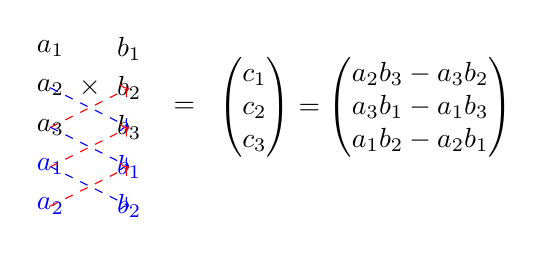
\begin{tikzpicture}

        \node at (0, 0) {\(a_1\)};
        \node at (0, -0.5) {\(a_2\)};
        \node at (0, -1) {\(a_3\)};
        \node at (0.5, -0.5) {\(\times\)};
        \node at (1, 0) {\(b_1\)};
        \node at (1, -0.5) {\(b_2\)};
        \node at (1, -1) {\(b_3\)};

        \node[text=blue] at (0, -1.5) {\(a_1\)};
        \node[text=blue] at (0, -2) {\(a_2\)};

        \node[text=blue] at (1, -1.5) {\(b_1\)};
        \node[text=blue] at (1, -2) {\(b_2\)};

        % Pfeile für c_1
        \draw[dashed, blue, ->] (0,-0.5) -- (1, -1);   % a_2 * b_3
        \draw[dashed, red, ->] (0,-1) -- (1, -0.5);   % a_3 * b_2

        % Pfeile für c_2
        \draw[dashed, blue, ->] (0,-1) -- (1, -1.5);  % a_3 * b_1 (rep.)
        \draw[dashed, red, ->] (0,-1.5) -- (1, -1);  % a_1 (rep.) * b_3

        % Pfeile für c_3
        \draw[dashed, blue, ->] (0,-1.5) -- (1, -2); % a_1 (rep.) * b_2 (rep.)
        \draw[dashed, red, ->] (0,-2) -- (1, -1.5); % a_2 (rep.) * b_1 (rep.)

        \node at (1.7, -0.75) {\(=\)};
        \node at (4, -0.75) {\(\begin{pmatrix}
                c_1 \\ c_2 \\ c_3
            \end{pmatrix} = \begin{pmatrix}
                a_2b_3 - a_3b_2 \\
                a_3b_1 - a_1b_3 \\
                a_1b_2 - a_2b_1
            \end{pmatrix}\)}; % Ergebnisvektor etwas verschoben für bessere Lesbarkeit

    \end{tikzpicture}
    \caption{Berechnungsschema des Kreuzprodukts nach der Regel von Sarrus. Die ersten beiden Komponenten jedes Vektors werden unterhalb wiederholt (hier in blau dargestellt).}
    \label{fig:kreuzprodukt_sarrus_user}
\end{figure}

\subsubsection*{Erläuterung der Zeichnung zur Kreuzproduktberechnung}

Die oben dargestellte Grafik (siehe Abbildung
\ref{fig:kreuzprodukt_sarrus_user}) veranschaulicht eine Methode zur Berechnung
des Kreuzprodukts \(\vec{c} = \vec{a} \times \vec{b}\), die oft als Erweiterung
der Regel von Sarrus bezeichnet wird. So wird die Zeichnung verwendet:

\begin{enumerate}
    \item \textbf{Komponenten aufschreiben:} Die Komponenten der beiden Vektoren \(\vec{a} = \begin{pmatrix} a_1 \\ a_2 \\ a_3 \end{pmatrix}\) und \(\vec{b} = \begin{pmatrix} b_1 \\ b_2 \\ b_3 \end{pmatrix}\) werden nebeneinander notiert.
    \item \textbf{Komponenten wiederholen:} Die ersten beiden Komponenten jedes Vektors (\(a_1, a_2\) und \(b_1, b_2\)) werden unterhalb der ursprünglichen drei Komponenten erneut aufgeschrieben. In der Zeichnung sind diese wiederholten Komponenten zur Verdeutlichung blau markiert.
    \item \textbf{Produkte bilden und Komponenten berechnen:} Nun werden die Komponenten des Ergebnisvektors \(\vec{c} = \begin{pmatrix} c_1 \\ c_2 \\ c_3 \end{pmatrix}\) durch diagonale Multiplikation bestimmt:
          \begin{itemize}
              \item \textbf{Für \(c_1\):}
                    Man betrachtet die zweite und dritte Zeile der ursprünglichen Komponenten.
                    Die blau gestrichelte Linie von \(a_2\) nach \(b_3\) zeigt das Produkt \(+a_2 b_3\).
                    Die rot gestrichelte Linie von \(a_3\) nach \(b_2\) zeigt das Produkt \(-a_3 b_2\).
                    Somit ist \(c_1 = a_2 b_3 - a_3 b_2\).

              \item \textbf{Für \(c_2\):}
                    Man betrachtet die dritte Zeile der ursprünglichen Komponenten (\(a_3, b_3\)) und die erste Zeile der wiederholten Komponenten (\(a_1, b_1\), in blau).
                    Die blau gestrichelte Linie von \(a_3\) (Original) nach \(b_1\) (blau, wiederholt) zeigt das Produkt \(+a_3 b_1\).
                    Die rot gestrichelte Linie von \(a_1\) (blau, wiederholt) nach \(b_3\) (Original) zeigt das Produkt \(-a_1 b_3\).
                    Somit ist \(c_2 = a_3 b_1 - a_1 b_3\).

              \item \textbf{Für \(c_3\):}
                    Man betrachtet die erste und zweite Zeile der wiederholten Komponenten (alle blau).
                    Die blau gestrichelte Linie von \(a_1\) (blau, wiederholt) nach \(b_2\) (blau, wiederholt) zeigt das Produkt \(+a_1 b_2\).
                    Die rot gestrichelte Linie von \(a_2\) (blau, wiederholt) nach \(b_1\) (blau, wiederholt) zeigt das Produkt \(-a_2 b_1\).
                    Somit ist \(c_3 = a_1 b_2 - a_2 b_1\).
          \end{itemize}
    \item \textbf{Ergebnisvektor:} Die berechneten Werte \(c_1, c_2, c_3\) bilden die Komponenten des Kreuzproduktvektors, wie auf der rechten Seite der Zeichnung dargestellt.
\end{enumerate}

	\chapter{Matrizen}

Eine Matrix ist eine rechteckige Anordnung von Zahlen oder anderen mathematischen Objekten, die in Zeilen und Spalten organisiert sind. Die Notation $M \in \mathbb{R}^{m \times n}$ wird hier verwendet, um eine Matrix zu beschreiben, welche $n$ Zeilen (Höhe) und $m$ Spalten (Breite) besitzt. Die einzelnen Elemente der Matrix werden mit $a_{ij}$ bezeichnet, wobei $i$ den Zeilenindex (von $1$ bis $n$) und $j$ den Spaltenindex (von $1$ bis $m$) angibt.

Eine solche Matrix $M$ mit $n$ Zeilen und $m$ Spalten hat die allgemeine Form:
\[
   M = \begin{pmatrix}
   a_{11} & a_{12} & \cdots & a_{1m} \\
   a_{21} & a_{22} & \cdots & a_{2m} \\
   \vdots & \vdots & \ddots & \vdots \\
   a_{n1} & a_{n2} & \cdots & a_{nm}
   \end{pmatrix}
\]
Eine Matrix kann auch als eine Zusammenfassung von Spaltenvektoren (wenn jede Spalte als Vektor betrachtet wird) oder Zeilenvektoren (wenn jede Zeile als Vektor betrachtet wird) angesehen werden.

\section{Matrix-Vektor-Produkt}

Das Produkt einer Matrix $M \in \mathbb{R}^{n \times m}$ (also $n$ Zeilen, $m$ Spalten) mit einem Spaltenvektor $V \in \mathbb{R}^{m \times 1}$ (also ein Vektor mit $m$ Elementen) ist ein neuer Spaltenvektor $W \in \mathbb{R}^{n \times 1}$ (also ein Vektor mit $n$ Elementen).
Die Multiplikation ist nur definiert, wenn die Anzahl der Spalten der Matrix $M$ gleich der Anzahl der Zeilen (Elemente) des Vektors $V$ ist. Hier müssen also beide die Dimension $m$ aufweisen.

Sei $M = \begin{pmatrix}
a_{11} & a_{12} & \cdots & a_{1m} \\
a_{21} & a_{22} & \cdots & a_{2m} \\
\vdots & \vdots & \ddots & \vdots \\
a_{n1} & a_{n2} & \cdots & a_{nm}
\end{pmatrix}$ und $V = \begin{pmatrix} v_1 \\ v_2 \\ \vdots \\ v_m \end{pmatrix}$.

Das Matrix-Vektor-Produkt $MV$ wird berechnet, indem das Skalarprodukt jeder Zeile der Matrix $M$ mit dem Vektor $V$ gebildet wird:
\[
   MV = \begin{pmatrix}
   a_{11}v_1 + a_{12}v_2 + \cdots + a_{1m}v_m \\
   a_{21}v_1 + a_{22}v_2 + \cdots + a_{2m}v_m \\
   \vdots \\
   a_{n1}v_1 + a_{n2}v_2 + \cdots + a_{nm}v_m
   \end{pmatrix} = \begin{pmatrix} \sum_{j=1}^{m} a_{1j}v_j \\ \sum_{j=1}^{m} a_{2j}v_j \\ \vdots \\ \sum_{j=1}^{m} a_{nj}v_j \end{pmatrix}
\]
Das Ergebnis ist ein Vektor mit $n$ Elementen.

\section{Diagonalmatrix}

Eine Diagonalmatrix ist eine quadratische Matrix, d.h. sie besitzt gleich viele Zeilen wie Spalten ($n=m$). Bei einer Diagonalmatrix sind alle Elemente außerhalb der Hauptdiagonalen (die von links oben nach rechts unten verläuft) gleich Null. Nur die Elemente auf der Hauptdiagonalen können von Null verschieden sein.

Eine Diagonalmatrix $D \in \mathbb{R}^{n \times n}$ hat die Form:
\[
D = \begin{pmatrix}
d_{11} & 0 & \cdots & 0 \\
0 & d_{22} & \cdots & 0 \\
\vdots & \vdots & \ddots & \vdots \\
0 & 0 & \cdots & d_{nn}
\end{pmatrix}
\]
Beispiel einer $3 \times 3$ Diagonalmatrix (hier ist $n=m=3$):
\[
   D = \begin{pmatrix}
   1 & 0 & 0 \\
   0 & 2 & 0 \\
   0 & 0 & 7
   \end{pmatrix}
   \in \mathbb{R}^{3 \times 3}
\]
Das Matrix-Vektor-Produkt mit einer Diagonalmatrix ist besonders einfach zu berechnen. Jedes Element des Vektors wird mit dem entsprechenden Diagonalelement der Matrix multipliziert:
Sei $V = \begin{pmatrix}v_1\\v_2\\v_3\end{pmatrix}$. Dann ist
\[
   D V = \begin{pmatrix}
   1 & 0 & 0 \\
   0 & 2 & 0 \\
   0 & 0 & 7
   \end{pmatrix}
   \begin{pmatrix}v_1\\v_2\\v_3\end{pmatrix}
   = \begin{pmatrix}1 \cdot v_1\\2 \cdot v_2\\7 \cdot v_3\end{pmatrix}
\]

\subsection{Einheitsmatrix}

Die Einheitsmatrix, oft mit $I$ oder $I_n$ (wobei $n$ die Dimension angibt) bezeichnet, ist eine spezielle Diagonalmatrix. Bei der Einheitsmatrix sind alle Elemente auf der Hauptdiagonalen gleich Eins, und alle anderen Elemente sind Null. Sie ist ebenfalls quadratisch.

Beispiel der $3 \times 3$ Einheitsmatrix $I_3$:
\[
   I_3 = \begin{pmatrix}
   1 & 0 & 0 \\
   0 & 1 & 0 \\
   0 & 0 & 1
   \end{pmatrix}
   \in \mathbb{R}^{3 \times 3}
\]
Die Multiplikation einer Matrix oder eines Vektors mit der Einheitsmatrix passender Dimension verändert diese nicht (d.h. $IM = M$ und $Iv = v$). Sie ist das neutrale Element der Matrizenmultiplikation.

\section{Drehmatrizen}

Drehmatrizen sind quadratische Matrizen, die verwendet werden, um Vektoren um einen Ursprung (in 2D) oder eine Achse (in 3D) um einen bestimmten Winkel zu drehen.

\subsection*{Drehmatrix in $\mathbb{R}^2$}
Eine Drehung eines Vektors in der Ebene ($\mathbb{R}^2$) um den Ursprung um den Winkel $\alpha$ (üblicherweise gegen den Uhrzeigersinn) wird durch die folgende $2 \times 2$-Matrix $R(\alpha)$ beschrieben:
\[
   R(\alpha) = \begin{pmatrix}
       \cos(\alpha) & -\sin(\alpha) \\
       \sin(\alpha) & \cos(\alpha)
   \end{pmatrix}
\]
Wird ein Vektor $v = \begin{pmatrix} x \\ y \end{pmatrix}$ mit dieser Matrix multipliziert, $v' = R(\alpha)v$, so ist $v'$ der um $\alpha$ gedrehte Vektor.

\subsection*{Drehmatrizen in $\mathbb{R}^3$}
Im dreidimensionalen Raum ($\mathbb{R}^3$) erfolgen Drehungen typischerweise um die Koordinatenachsen ($x, y, z$). Die entsprechenden Drehmatrizen sind $3 \times 3$-Matrizen.

\subsubsection*{Drehung um die $x$-Achse}
Eine Drehung um den Winkel $\alpha$ um die $x$-Achse wird durch die Matrix $R_x(\alpha)$ repräsentiert:
\[
   R_x(\alpha) = \begin{pmatrix}
       1 & 0 & 0 \\
       0 & \cos(\alpha) & -\sin(\alpha) \\
       0 & \sin(\alpha) & \cos(\alpha)
   \end{pmatrix}
\]

\subsubsection*{Drehung um die $y$-Achse}
Eine Drehung um den Winkel $\alpha$ (oder $\beta$ zur Unterscheidung) um die $y$-Achse wird durch die Matrix $R_y(\alpha)$ repräsentiert:
\[
   R_y(\alpha) = \begin{pmatrix}
       \cos(\alpha) & 0 & \sin(\alpha) \\
       0 & 1 & 0 \\
       -\sin(\alpha) & 0 & \cos(\alpha)
   \end{pmatrix}
\]

\subsubsection*{Drehung um die $z$-Achse}
Eine Drehung um den Winkel $\alpha$ (oder $\gamma$) um die $z$-Achse wird durch die Matrix $R_z(\alpha)$ repräsentiert:
\[
   R_z(\alpha) = \begin{pmatrix}
       \cos(\alpha) & -\sin(\alpha) & 0 \\
       \sin(\alpha) & \cos(\alpha) & 0 \\
       0 & 0 & 1
   \end{pmatrix}
\]

\subsection{Drehung um mehrere Achsen}
Wenn ein Vektor in $\mathbb{R}^3$ nacheinander um mehrere Achsen gedreht werden soll, können die entsprechenden Drehmatrizen miteinander multipliziert werden (siehte \nameref{matrix_multiplitzieren}). Das Ergebnis dieser Matrizenmultiplikation ist eine einzelne Matrix, die die Gesamttransformation (also die verkettete Drehung) darstellt.
Wird beispielsweise zuerst eine Drehung $R_1$ und danach eine Drehung $R_2$ auf einen Vektor $v$ angewendet, so ist der transformierte Vektor $v' = R_2 (R_1 v) = (R_2 R_1) v$. Die Gesamttransformationsmatrix ist $R_{ges} = R_2 R_1$.
Es ist wichtig zu beachten, dass die Matrizenmultiplikation im Allgemeinen nicht kommutativ ist, d.h. die Reihenfolge der Multiplikation (und somit der Drehungen) ist entscheidend ($R_2 R_1 \neq R_1 R_2$ im Allgemeinen). Die Matrix, die der zuerst auszuführenden Drehung entspricht, steht im Produkt rechts.

\section{Spiegelungen}
	\chapter{Determinante}
\label{determinante}

Die Determinante ist eine spezielle Zahl, die einer quadratischen Matrix zugeordnet wird. Sie liefert wichtige Informationen über die Matrix und die lineare Transformation, die sie repräsentiert. Geometrisch kann die Determinante einer $n \times n$ Matrix als der Skalierungsfaktor des $n$-dimensionalen Volumens des Parallelepipeds interpretiert werden, das von den Spaltenvektoren (oder Zeilenvektoren) der Matrix aufgespannt wird. Ist die Determinante gleich null, so ist das Volumen null. Dies bedeutet, dass die Vektoren, welche die Matrix bilden, linear abhängig sind und die Transformation den Raum auf eine niedrigere Dimension abbildet (z.B. eine Ebene auf eine Gerade oder einen Punkt). Eine Determinante ist nur für quadratische Matrizen definiert.

\section{Determinante einer $2 \times 2$ Matrix}

Um die Determinante einer $2 \times 2$ Matrix $A = \begin{pmatrix} a & b \\ c & d \end{pmatrix}$ zu berechnen, werden ganz einfach die Diagonalen multipliziert und subtrahiert.
\[
    \det(A) = a \cdot d - c \cdot b
\]

\section{Determinanten von nicht $2 \times 2$ Matrizen}

Um die Determinante einer nicht $2 \times 2$ Matrix zu berechnen, gibt es im Wesentlichen drei Herangehensweisen:

\subsection{Regel von Sarrus}

Die Regel von Sarrus funktioniert \textbf{nur bei $3 \times 3$} Matrizen.

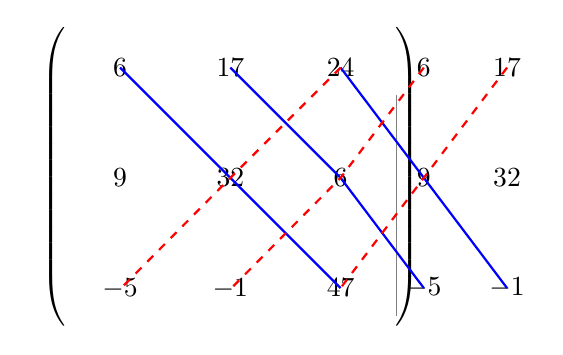
\begin{tikzpicture}[
    every node/.style={minimum size=0.7cm},
    positive/.style={blue, thick},
    negative/.style={red, thick, dashed}
  ]
  \matrix (m) [matrix of math nodes,
               nodes in empty cells,
               left delimiter=(, right delimiter=),
               column sep=0.7cm, row sep=0.7cm, % Abstand zwischen Zellen
               ampersand replacement=\&] % Wichtig für tikz-matrix
  {
    6 \& 17 \& 24 \\
    9 \& 32 \& 6 \\
    -5 \& -1 \& 47 \\
  };

  % Erweiterte Spalten (nur für die Visualisierung der Linien)
  \node at ($(m-1-3.east)!0.5!(m-1-3.east) + (0.7cm,0)$) (m-1-4) {$6$};
  \node at ($(m-2-3.east)!0.5!(m-2-3.east) + (0.7cm,0)$) (m-2-4) {$9$};
  \node at ($(m-3-3.east)!0.5!(m-3-3.east) + (0.7cm,0)$) (m-3-4) {$-5$};

  \node at ($(m-1-4.east)!0.5!(m-1-4.east) + (0.7cm,0)$) (m-1-5) {$17$};
  \node at ($(m-2-4.east)!0.5!(m-2-4.east) + (0.7cm,0)$) (m-2-5) {$32$};
  \node at ($(m-3-4.east)!0.5!(m-3-4.east) + (0.7cm,0)$) (m-3-5) {$-1$};

  % Vertikale Trennlinie (optional)
  \draw[gray, thin] ($(m-1-3.east)!0.5!(m-2-3.east) + (0.35cm,0.35cm)$) -- ($(m-3-3.east) + (0.35cm,-0.35cm)$);


  % Positive Diagonalen (blau, durchgezogen)
  \draw[positive] (m-1-1.center) -- (m-2-2.center) -- (m-3-3.center); % a-e-i
  \draw[positive] (m-1-2.center) -- (m-2-3.center) -- (m-3-4.center); % b-f-g (auf erweiterter Spalte)
  \draw[positive] (m-1-3.center) -- (m-2-4.center) -- (m-3-5.center); % c-d-h (auf erweiterter Spalte)

  % Negative Diagonalen (rot, gestrichelt)
  \draw[negative] (m-1-3.center) -- (m-2-2.center) -- (m-3-1.center); % c-e-g
  \draw[negative] (m-1-4.center) -- (m-2-3.center) -- (m-3-2.center); % a-f-h (auf erweiterter Spalte)
  \draw[negative] (m-1-5.center) -- (m-2-4.center) -- (m-3-3.center); % b-d-i (auf erweiterter Spalte)

\end{tikzpicture}

\bigskip % Etwas Abstand

Die Zahlen an den Linien werden multipliziert. Blaue Linien werden miteinander addiert und Rote subtrahiert.

\begin{align*}
    (6 \cdot 32 \cdot 47) + (17 \cdot 6 \cdot (-5)) + (24 \cdot 9 \cdot (-1)) \\
    - ((-5) \cdot 32 \cdot 24) - ((-1) \cdot 6 \cdot 6) - (47 \cdot 9 \cdot 17) \\
    = 9024 - 510 - 216 - (-3840) - (-36) - 7191 \\
    = 9024 - 510 - 216 + 3840 + 36 - 7191 \\
    = 4983
\end{align*}

\subsection{Leibniz-Formel (nicht prüfungsrelevant)}

Die Leibniz-Formel ist eine allgemeine Definition der Determinante für eine $n \times n$-Matrix $A=(a_{ij})$. Die Determinante wird als eine Summe über alle möglichen Permutationen der Spaltenindizes berechnet:
\[ \det(A) = \sum_{\sigma \in S_n} \text{sgn}(\sigma) \prod_{i=1}^{n} a_{i, \sigma(i)} \]
Hierbei ist:
\begin{itemize}
    \item $S_n$ die Menge aller Permutationen der Zahlen $\{1, 2, \ldots, n\}$. Eine Permutation $\sigma$ ist eine bijektive Abbildung dieser Menge auf sich selbst; $\sigma(i)$ ist das $i$-te Element in einer Anordnung der Zahlen $1, \ldots, n$.
    \item $\text{sgn}(\sigma)$ das Signum (Vorzeichen) der Permutation $\sigma$. Es ist $+1$, wenn die Permutation durch eine gerade Anzahl von Vertauschungen zweier Elemente (Transpositionen) aus der Grundreihenfolge $(1, 2, \ldots, n)$ hervorgeht. Es ist $-1$, wenn sie durch eine ungerade Anzahl von Vertauschungen hervorgeht. Alternativ kann das Signum über die Anzahl $k$ der Fehlstände (Inversionen) der Permutation berechnet werden als $\text{sgn}(\sigma) = (-1)^k$. Ein Fehlstand ist ein Paar von Indizes $(i,j)$ derart, dass $i < j$ ist, aber $\sigma(i) > \sigma(j)$ gilt.
    \item $\prod_{i=1}^{n} a_{i, \sigma(i)}$ das Produkt von $n$ Matrixelementen $a_{1, \sigma(1)} \cdot a_{2, \sigma(2)} \cdot \ldots \cdot a_{n, \sigma(n)}$. Dabei wird aus jeder Zeile $i$ genau ein Element ausgewählt, und zwar aus der Spalte $\sigma(i)$, sodass auch aus jeder Spalte genau ein Element stammt.
\end{itemize}
Für $n=2$ und $A = \begin{pmatrix} a_{11} & a_{12} \\ a_{21} & a_{22} \end{pmatrix}$ ergibt sich: $S_2$ enthält die Permutationen $\sigma_1 = (1,2)$ (Identität, $\sigma_1(1)=1, \sigma_1(2)=2$) und $\sigma_2 = (2,1)$ (Vertauschung, $\sigma_2(1)=2, \sigma_2(2)=1$).
\begin{itemize}
    \item $\sigma_1 = (1,2)$: Anzahl Fehlstände = 0. $\text{sgn}(\sigma_1)=(-1)^0=+1$. Term: $a_{1\sigma_1(1)}a_{2\sigma_1(2)} = a_{11}a_{22}$.
    \item $\sigma_2 = (2,1)$: Ein Fehlstand: $(1,2)$, da $1<2$ aber $\sigma_2(1)=2 > \sigma_2(2)=1$. $\text{sgn}(\sigma_2)=(-1)^1=-1$. Term: $a_{1\sigma_2(1)}a_{2\sigma_2(2)} = a_{12}a_{21}$.
\end{itemize}
Somit ist $\det(A) = (+1) \cdot a_{11}a_{22} + (-1) \cdot a_{12}a_{21} = a_{11}a_{22} - a_{12}a_{21}$. Dies entspricht der bekannten Formel für $2 \times 2$-Matrizen.

\subsubsection*{Beispiel für eine $3 \times 3$-Matrix}
Betrachtet sei die Matrix $A = \begin{pmatrix} 1 & 2 & 3 \\ 0 & 4 & 5 \\ 1 & 0 & 6 \end{pmatrix}$.
Für $n=3$ gibt es $3! = 6$ Permutationen in $S_3$. Die Elemente sind $a_{11}=1, a_{12}=2, a_{13}=3, a_{21}=0, a_{22}=4, a_{23}=5, a_{31}=1, a_{32}=0, a_{33}=6$.

\begin{enumerate}
    \item $\sigma_1 = (1,2,3)$ (d.h. $1 \mapsto 1, 2 \mapsto 2, 3 \mapsto 3$). Fehlstände: 0. $\text{sgn}(\sigma_1)=+1$. \\
    Produkt: $a_{11}a_{22}a_{33} = 1 \cdot 4 \cdot 6 = 24$. Term: $(+1) \cdot 24 = 24$.
    \item $\sigma_2 = (1,3,2)$ (d.h. $1 \mapsto 1, 2 \mapsto 3, 3 \mapsto 2$). Fehlstand: $(2,3)$ (weil $2<3$, aber $\sigma_2(2)=3 > \sigma_2(3)=2$). Anzahl Fehlstände: 1. $\text{sgn}(\sigma_2)=-1$. \\
    Produkt: $a_{11}a_{23}a_{32} = 1 \cdot 5 \cdot 0 = 0$. Term: $(-1) \cdot 0 = 0$.
    \item $\sigma_3 = (2,1,3)$ (d.h. $1 \mapsto 2, 2 \mapsto 1, 3 \mapsto 3$). Fehlstand: $(1,2)$ (weil $1<2$, aber $\sigma_3(1)=2 > \sigma_3(2)=1$). Anzahl Fehlstände: 1. $\text{sgn}(\sigma_3)=-1$. \\
    Produkt: $a_{12}a_{21}a_{33} = 2 \cdot 0 \cdot 6 = 0$. Term: $(-1) \cdot 0 = 0$.
    \item $\sigma_4 = (2,3,1)$ (d.h. $1 \mapsto 2, 2 \mapsto 3, 3 \mapsto 1$). Fehlstände: $(1,3)$ (weil $1<3$, $\sigma_4(1)=2 > \sigma_4(3)=1$); $(2,3)$ (weil $2<3$, $\sigma_4(2)=3 > \sigma_4(3)=1$). Anzahl Fehlstände: 2. $\text{sgn}(\sigma_4)=+1$. \\
    Produkt: $a_{12}a_{23}a_{31} = 2 \cdot 5 \cdot 1 = 10$. Term: $(+1) \cdot 10 = 10$.
    \item $\sigma_5 = (3,1,2)$ (d.h. $1 \mapsto 3, 2 \mapsto 1, 3 \mapsto 2$). Fehlstände: $(1,2)$ (weil $1<2$, $\sigma_5(1)=3 > \sigma_5(2)=1$); $(1,3)$ (weil $1<3$, $\sigma_5(1)=3 > \sigma_5(3)=2$). Anzahl Fehlstände: 2. $\text{sgn}(\sigma_5)=+1$. \\
    Produkt: $a_{13}a_{21}a_{32} = 3 \cdot 0 \cdot 0 = 0$. Term: $(+1) \cdot 0 = 0$.
    \item $\sigma_6 = (3,2,1)$ (d.h. $1 \mapsto 3, 2 \mapsto 2, 3 \mapsto 1$). Fehlstände: $(1,2)$ (weil $1<2$, $\sigma_6(1)=3 > \sigma_6(2)=2$); $(1,3)$ (weil $1<3$, $\sigma_6(1)=3 > \sigma_6(3)=1$); $(2,3)$ (weil $2<3$, $\sigma_6(2)=2 > \sigma_6(3)=1$). Anzahl Fehlstände: 3. $\text{sgn}(\sigma_6)=-1$. \\
    Produkt: $a_{13}a_{22}a_{31} = 3 \cdot 4 \cdot 1 = 12$. Term: $(-1) \cdot 12 = -12$.
\end{enumerate}
Die Determinante ist die Summe dieser Terme:
\[ \det(A) = 24 + 0 + 0 + 10 + 0 - 12 = 22 \]
Dies ist dasselbe Ergebnis, das man mit der Regel von Sarrus für $3 \times 3$-Matrizen erhalten würde. Die Leibniz-Formel ist jedoch allgemeingültig für Matrizen beliebiger quadratischer Größe, während die Sarrus-Regel nur für $3 \times 3$-Matrizen gilt.

\subsection{Kästchenregel}

Bei der Kästchenregel, auch bekannt als Determinantenformel für Blockmatrizen, kann die Determinante einer Matrix berechnet werden, indem die Matrix in Blöcke (Kästchen) unterteilt wird. Dies ist besonders nützlich, wenn einige der Blöcke Nullmatrizen sind.
Für eine Blockmatrix der Form
\[ M = \begin{pmatrix} A & B \\ 0 & D \end{pmatrix} \quad \text{oder} \quad M = \begin{pmatrix} A & 0 \\ C & D \end{pmatrix} \]
wobei $A$ und $D$ quadratische Matrizen sind (und $0$ eine Nullmatrix passender Größe ist), ist die Determinante gegeben durch
\[ \det(M) = \det(A) \cdot \det(D) \]
Diese Regel vereinfacht die Berechnung erheblich, wenn Matrizen in eine solche obere oder untere Blockdreiecksform gebracht werden können. Die Kästchenregel bietet sich besonders bei $\mathbb{R}^{n \times n}$ Matrizen an, bei denen $n \geq 4$ ist und eine geeignete Blockstruktur vorliegt oder erzeugt werden kann.

\begin{longtable}{p{10cm}}

    \hline
    \multicolumn{1}{c}{\textbf{Linearkombination}} \\
    \hline
    \endfirsthead

    \hline
    \multicolumn{1}{c}{\tablename\ \thetable\ -- \textit{Fortführung von vorherier Seite}} \\
    \hline
    \multicolumn{1}{c}{\textbf{Linearkombination}} \\
    \hline
    \endhead

    \hline
    \multicolumn{1}{r}{\textit{Fortsetzung siehe nächste Seite}} \\
    \endfoot

    \hline
    \endlastfoot

    $\displaystyle\begin{pmatrix} % Matrix statt array für pmatrix-Stil
    1 & 0 & 2 & 0 \\
    1 & 2 & 9 & 0 \\
    2 & 0 & 1 & 5 \\
    1 & 1 & 1 & 1
    \end{pmatrix}$\\\hline
    I und IV tauschen (Vorzeichenwechsel für Determinante: $\cdot (-1)$) \\\hline\pagebreak[0] % Hinweis auf Vorzeichenwechsel


    $\displaystyle\begin{pmatrix}
    1 & 1 & 1 & 1 \\
    1 & 2 & 9 & 0 \\
    2 & 0 & 1 & 5 \\
    1 & 0 & 2 & 0
    \end{pmatrix}$\\\hline
    II - I $\rightarrow$ II \\ % Korrekte Notation für Zeilenumformung
    III - 2I $\rightarrow$ III \\
    IV - I $\rightarrow$ IV \\\hline\pagebreak[0]

    $\displaystyle\begin{pmatrix}
    1 & 1 & 1 & 1 \\
    0 & 1 & 8 & -1 \\
    0 & -2 & -1 & 3 \\
    0 & -1 & 1 & -1
    \end{pmatrix}$\\\hline
    III + 2II $\rightarrow$ III \\
    IV + II $\rightarrow$ IV \\\hline\pagebreak[0]

    $\displaystyle\begin{pmatrix}
    1 & 1 & 1 & 1 \\
    0 & 1 & 8 & -1 \\
    0 & 0 & 15 & 1 \\
    0 & 0 & 9 & -2
    \end{pmatrix}$\\\hline
    % Hier ist die Matrix B aus dem Beispiel erreicht, aber der Gauß-Algorithmus könnte weitergeführt werden.
    % Die gezeigte Matrix ist B = \left( \begin{array}{cc|cc} 1 & 1 & 1 & 1 \\ 0 & 1 & 8 & -1 \\ \hline 0 & 0 & 15 & 1 \\ 0 & 0 & 9 & -2 \end{array} \right)
    % und nicht die ursprüngliche Matrix A.
    % Die Determinante dieser umgeformten Matrix ist (-1) * det(ursprüngliche Matrix).

\end{longtable}

Die im Beispiel umgeformte Matrix (nennen wir sie $M'$) nach Zeilentausch und Umformungen ist:
\[
M' = \begin{pmatrix}
    1 & 1 & 1 & 1 \\
    0 & 1 & 8 & -1 \\
    0 & 0 & 15 & 1 \\
    0 & 0 & 9 & -2
    \end{pmatrix}
\]
Diese Matrix hat eine obere Dreiecksblockstruktur, wenn man sie betrachtet als:
\[
M' = \left( \begin{array}{cc|cc}
1 & 1 & 1 & 1 \\
0 & 1 & 8 & -1 \\
\hline
0 & 0 & 15 & 1 \\
0 & 0 & 9 & -2
\end{array} \right)
= \begin{pmatrix} A' & B' \\ 0 & D' \end{pmatrix}
\]
wobei $A' = \begin{pmatrix} 1 & 1 \\ 0 & 1 \end{pmatrix}$ und $D' = \begin{pmatrix} 15 & 1 \\ 9 & -2 \end{pmatrix}$.
Die Determinante ist $\det(M') = \det(A') \cdot \det(D')$.

\bigskip

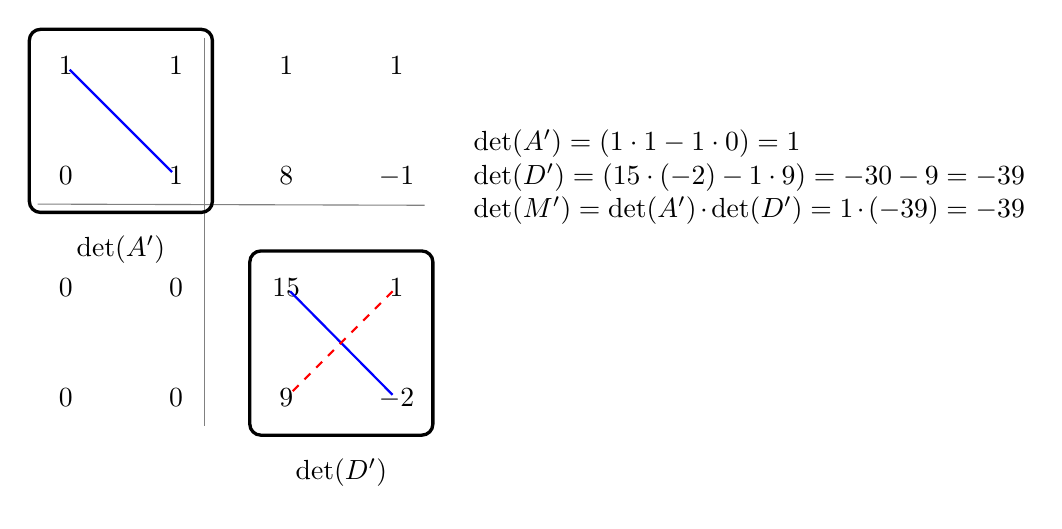
\begin{tikzpicture}[
    every node/.style={minimum size=0.7cm},
    positive/.style={blue, thick},
    negative/.style={red, thick, dashed},
    block/.style={draw, very thick, rounded corners, inner sep=3pt}
  ]
  \matrix (m) [matrix of math nodes,
               nodes in empty cells,
               column sep=0.7cm, row sep=0.7cm,
               ampersand replacement=\&]
  {
    1 \& 1 \& 1 \& 1 \\ % Zeile 1 von M'
    0 \& 1 \& 8 \& -1 \\ % Zeile 2 von M'
    0 \& 0 \& 15 \& 1 \\ % Zeile 3 von M'
    0 \& 0 \& 9 \& -2 \\ % Zeile 4 von M'
  };

  \draw[gray, thin] (m-2-1.south west) -- (m-2-4.south east);
  \draw[gray, thin] (m-1-2.north east) -- (m-4-2.south east);

  \node[block, fit=(m-1-1) (m-2-2), label={[yshift=-0.1cm]below:$\det(A')$}] (blockA) {};
  \node[block, fit=(m-3-3) (m-4-4), label={[yshift=-0.1cm]below:$\det(D')$}] (blockD) {};

  \draw[positive, shorten >=2pt, shorten <=2pt] (m-1-1.center) -- (m-2-2.center); % 1*1
  % keine negative Diagonale für A', da 0*1=0

  \draw[positive, shorten >=2pt, shorten <=2pt] (m-3-3.center) -- (m-4-4.center); % 15*(-2)
  \draw[negative, shorten >=2pt, shorten <=2pt] (m-3-4.center) -- (m-4-3.center); % 1*9

  \node[anchor=west, text width=7cm, at={($(m-2-4.east)+(0.5cm,0)$)}] (formel)
    {
     $\det(A') = (1 \cdot 1 - 1 \cdot 0) = 1$ \\
     $\det(D') = (15 \cdot (-2) - 1 \cdot 9) = -30 - 9 = -39$ \\
     $\det(M') = \det(A') \cdot \det(D') = 1 \cdot (-39) = -39$
    };
\end{tikzpicture}

Da die Matrix $M'$ aus der ursprünglichen Matrix durch einen Zeilentausch und elementare Zeilenumformungen, die die Determinante nicht ändern (Addition eines Vielfachen einer Zeile zu einer anderen), hervorgegangen ist, gilt: $\det(\text{ursprüngliche Matrix}) = (-1) \cdot \det(M') = (-1) \cdot (-39) = 39$.

\section{Transponiertheit}
\begin{itemize}
    \item Die Transponierte einer Matrix \(A\), bezeichnet als \(A^T\), entsteht durch Spiegelung der Elemente an der Hauptdiagonalen.
    \item Das Element \(A_{m,n}\) der Ursprungsmatrix wird zum Element \(A_{n,m}\) der transponierten Matrix.
    \item Eine \(m \times n\)-Matrix wird zu einer \(n \times m\)-Matrix.
    \item \textbf{Beispiel:}
    \[
    A = \begin{pmatrix}
        1 & 2 & 3 \\
        4 & 5 & 6
    \end{pmatrix}
    \rightarrow
    A^T = \begin{pmatrix}
        1 & 4 \\
        2 & 5 \\
        3 & 6
    \end{pmatrix}
    \]
\end{itemize}
	\chapter{Matritzen Multiplitzieren}
\label{matrix_multiplitzieren}

Zwei Matritzen $A$ und $B$ dürfen nur miteinander Multiplitziert werden, wenn $A$ so viele Spalten hat, wie $B$ Zeilen. Sein die Matritzen $A = \begin{pmatrix}
    1 & 3 \\
    0 & 1 \\
    1 & 3
\end{pmatrix}, B = \begin{pmatrix}
    1 & 2 \\
    2 & 4
\end{pmatrix}$, so werden sie wie folgt Multiplitziert

\begin{align*}
    A \cdot B \\
    \begin{pmatrix}
        1 & 3 \\
        0 & 1 \\
        1 & 3
    \end{pmatrix} \cdot \begin{pmatrix}
        1 & 2 \\
        2 & 4
    \end{pmatrix} \\
    = \begin{pmatrix}
        1 \cdot 1 + 3 \cdot 2 & 1 \cdot 3 + 3 \cdot 4 \\
        0 \cdot 1 + 1 \cdot 2 & 0 \cdot 3 + 1 \cdot 4 \\
        1 \cdot 1 + 3 \cdot 2 & 1 \cdot 3 + 3 \cdot 4
    \end{pmatrix} \\
    = \begin{pmatrix}
        7 & 15 \\
        2 & 4 \\
        7 & 15
    \end{pmatrix}
\end{align*}
	\chapter{Matrizen Invertieren}

Die Inverse einer quadratischen Matrix \(A\) ist eine Matrix \(A^{-1}\), sodass
das Produkt von \(A\) und \(A^{-1}\) die Einheitsmatrix \(I\) ergibt:
\[ AA^{-1} = A^{-1}A = I \]
Eine Methode zur Berechnung der Inversen einer Matrix ist das
\nameref{gauss_jordan_verfahren}. Bei diesem Verfahren wird die zu
invertierende Matrix \(A\) um die Einheitsmatrix \(I\) derselben Dimension
erweitert, sodass eine Matrix \([A|I]\) entsteht. Durch elementare
Zeilenumformungen wird der linke Teil \(A\) in die reduzierte Zeilenstufenform
überführt. Wenn \(A\) in die Einheitsmatrix \(I\) transformiert werden kann,
ist die resultierende rechte Seite die Inverse \(A^{-1}\), also \([I|A^{-1}]\).

Eine notwendige und hinreichende Bedingung für die Invertierbarkeit einer
quadratischen Matrix ist, dass ihre \nameref{determinante} ungleich Null ist.
Ist \(\det(A) = 0\), so ist die Matrix singulär und besitzt keine Inverse.

\section{Beispiel}

Es soll die Inverse der Matrix \(A\) bestimmt werden:
\[ A = \begin{pmatrix}
        1 & 2 & 3 \\
        0 & 1 & 4 \\
        5 & 6 & 0
    \end{pmatrix} \]
Zuerst wird die Determinante von \(A\) berechnet, um die Invertierbarkeit zu
prüfen. Nach der Regel von Sarrus (für 3x3-Matrizen):
\begin{align*}
    \det(A) & = (1 \cdot 1 \cdot 0) + (2 \cdot 4 \cdot 5) + (3 \cdot 0 \cdot 6)       \\
            & \quad - (5 \cdot 1 \cdot 3) - (6 \cdot 4 \cdot 1) - (0 \cdot 0 \cdot 2) \\
            & = 0 + 40 + 0 - 15 - 24 - 0                                              \\
            & = 1
\end{align*}
Da \(\det(A) = 1 \neq 0\), ist die Matrix \(A\) invertierbar.

Nun wird das Gauß-Jordan-Verfahren angewendet. Die erweiterte Matrix ist:
\[ \left[ A | I \right] = \left[ \begin{array}{ccc|ccc}
            1 & 2 & 3 & 1 & 0 & 0 \\
            0 & 1 & 4 & 0 & 1 & 0 \\
            5 & 6 & 0 & 0 & 0 & 1
        \end{array} \right] \]

\begin{longtable}{p{4cm}|p{3cm}}

    \hline
    \multicolumn{1}{c|}{\textbf{Matrix}} & \multicolumn{1}{c}{\textbf{Inverse}}            \\
    \hline
    \endfirsthead

    \hline
    \multicolumn{2}{c}{\tablename\ \thetable\ -- \textit{Fortführung von vorherier Seite}} \\
    \hline
    \multicolumn{1}{c|}{\textbf{Matrix}} & \multicolumn{1}{c}{\textbf{Inverse}}            \\
    \hline
    \endhead

    \hline
    \multicolumn{2}{r}{\textit{Fortsetzung siehe nächste Seite}}                           \\
    \endfoot

    \hline
    \endlastfoot

    $\displaystyle\begin{matrix}
                          1 & 2 & 3 \\
                          0 & 1 & 4 \\
                          5 & 6 & 0
                      \end{matrix}$         &
    $\displaystyle\begin{matrix}
                          1 & 0 & 0 \\
                          0 & 1 & 0 \\
                          0 & 0 & 1 \\
                      \end{matrix}$                                                            \\\hline
    \multicolumn{2}{p{\dimexpr4cm+3cm+2\tabcolsep\relax}}{Operation: III - 5I}             \\\hline\pagebreak[0]
    $\displaystyle\begin{matrix}
                          1 & 2  & 3   \\
                          0 & 1  & 4   \\
                          0 & -4 & -15
                      \end{matrix}$         &
    $\displaystyle\begin{matrix}
                          1  & 0 & 0 \\
                          0  & 1 & 0 \\
                          -5 & 0 & 1 \\
                      \end{matrix}$                                                            \\\hline
    \multicolumn{2}{p{\dimexpr4cm+3cm+2\tabcolsep\relax}}{Operation: III + 4II}            \\\hline\pagebreak[0]
    $\displaystyle\begin{matrix}
                          1 & 2 & 3 \\
                          0 & 1 & 4 \\
                          0 & 0 & 1
                      \end{matrix}$         &
    $\displaystyle\begin{matrix}
                          1  & 0 & 0 \\
                          0  & 1 & 0 \\
                          -5 & 4 & 1 \\
                      \end{matrix}$                                                            \\\hline
    \multicolumn{2}{p{\dimexpr4cm+3cm+2\tabcolsep\relax}}{Operation: I - 2II}              \\\hline\pagebreak[0]
    $\displaystyle\begin{matrix}
                          1 & 0 & -5 \\
                          0 & 1 & 4  \\
                          0 & 0 & 1
                      \end{matrix}$         &
    $\displaystyle\begin{matrix}
                          1  & -2 & 0 \\
                          0  & 1  & 0 \\
                          -5 & 4  & 1 \\
                      \end{matrix}$                                                            \\\hline
    \multicolumn{2}{p{\dimexpr4cm+3cm+2\tabcolsep\relax}}{Operation: II - 4III}            \\\hline\pagebreak[0]
    $\displaystyle\begin{matrix}
                          1 & 0 & -5 \\
                          0 & 1 & 0  \\
                          0 & 0 & 1
                      \end{matrix}$         &
    $\displaystyle\begin{matrix}
                          1  & -2  & 0  \\
                          20 & -15 & -4 \\
                          -5 & 4   & 1  \\
                      \end{matrix}$                                                            \\\hline
    \multicolumn{2}{p{\dimexpr4cm+3cm+2\tabcolsep\relax}}{Operation: I + 5III}             \\\hline\pagebreak[0]
    $\displaystyle\begin{matrix}
                          1 & 0 & 0 \\
                          0 & 1 & 0 \\
                          0 & 0 & 1
                      \end{matrix}$         &
    $\displaystyle\begin{matrix}
                          -24 & 18  & 5  \\
                          20  & -15 & -4 \\
                          -5  & 4   & 1  \\
                      \end{matrix}$                                                           \\\hline
\end{longtable}

Die linke Seite ist nun die Einheitsmatrix. Die rechte Seite ist die Inverse
\(A^{-1}\).
\[ A^{-1} = \begin{pmatrix}
        -24 & 18  & 5  \\
        20  & -15 & -4 \\
        -5  & 4   & 1
    \end{pmatrix} \]

\section{Umkehrabbildung}

Eine Matrix \(A \in \mathbb{R}^{n \times n}\) kann als eine lineare Abbildung
von \(\mathbb{R}^n\) nach \(\mathbb{R}^n\) interpretiert werden. Ein Vektor
\(\vec{x} \in \mathbb{R}^n\) wird durch die Matrix \(A\) auf einen Vektor
\(\vec{y} \in \mathbb{R}^n\) abgebildet:
\[ \vec{y} = A\vec{x} \]
Diese Abbildung \(f: \mathbb{R}^n \rightarrow \mathbb{R}^n\), \(\vec{x} \mapsto
A\vec{x}\) ist bijektiv (also sowohl injektiv als auch surjektiv) genau dann,
wenn die Matrix \(A\) invertierbar ist.

Wenn die Matrix \(A\) invertierbar ist, existiert eine Umkehrabbildung
\(f^{-1}: \mathbb{R}^n \rightarrow \mathbb{R}^n\). Diese Umkehrabbildung bildet
den Vektor \(\vec{y}\) zurück auf den ursprünglichen Vektor \(\vec{x}\) ab. Die
Abbildungsmatrix dieser Umkehrabbildung ist die Inverse \(A^{-1}\):
\[ \vec{x} = A^{-1}\vec{y} \]
Somit macht die Umkehrabbildung die ursprüngliche Abbildung rückgängig. Wendet
man beide Abbildungen nacheinander an, erhält man die identische Abbildung, bei
der jeder Vektor auf sich selbst abgebildet wird:
\[ A^{-1}(A\vec{x}) = (A^{-1}A)\vec{x} = I\vec{x} = \vec{x} \]
\[ A(A^{-1}\vec{y}) = (AA^{-1})\vec{y} = I\vec{y} = \vec{y} \]
Die Existenz einer Umkehrabbildung ist also direkt an die Invertierbarkeit der
Abbildungsmatrix \(A\) geknüpft, was wiederum bedeutet, dass \(\det(A) \neq 0\)
sein muss.

\subsection{Beispiel zur Umkehrabbildung}
Betrachten wir die Matrix \(A\) aus dem vorherigen Beispiel und ihre Inverse
\(A^{-1}\):
\[ A = \begin{pmatrix}
        1 & 2 & 3 \\
        0 & 1 & 4 \\
        5 & 6 & 0
    \end{pmatrix}, \quad
    A^{-1} = \begin{pmatrix}
        -24 & 18  & 5  \\
        20  & -15 & -4 \\
        -5  & 4   & 1
    \end{pmatrix} \]
Sei \(\vec{x} = \begin{pmatrix} 1 \\ 1 \\ 1 \end{pmatrix}\). Die Abbildung mit \(A\) ergibt:
\[ \vec{y} = A\vec{x} = \begin{pmatrix}
        1 & 2 & 3 \\
        0 & 1 & 4 \\
        5 & 6 & 0
    \end{pmatrix}
    \begin{pmatrix} 1 \\ 1 \\ 1 \end{pmatrix} =
    \begin{pmatrix}
        1 \cdot 1 + 2 \cdot 1 + 3 \cdot 1 \\
        0 \cdot 1 + 1 \cdot 1 + 4 \cdot 1 \\
        5 \cdot 1 + 6 \cdot 1 + 0 \cdot 1
    \end{pmatrix} =
    \begin{pmatrix} 6 \\ 5 \\ 11 \end{pmatrix} \]
Nun wird die Umkehrabbildung mit \(A^{-1}\) auf \(\vec{y}\) angewendet, um
\(\vec{x}\) zurückzuerhalten:
\[ A^{-1}\vec{y} = \begin{pmatrix}
        -24 & 18  & 5  \\
        20  & -15 & -4 \\
        -5  & 4   & 1
    \end{pmatrix}
    \begin{pmatrix} 6 \\ 5 \\ 11 \end{pmatrix} =
    \begin{pmatrix}
        -24 \cdot 6 + 18 \cdot 5 + 5 \cdot 11 \\
        20 \cdot 6 - 15 \cdot 5 - 4 \cdot 11  \\
        -5 \cdot 6 + 4 \cdot 5 + 1 \cdot 11
    \end{pmatrix} \]
\[ = \begin{pmatrix}
        -144 + 90 + 55 \\
        120 - 75 - 44  \\
        -30 + 20 + 11
    \end{pmatrix} =
    \begin{pmatrix} 1 \\ 1 \\ 1 \end{pmatrix} = \vec{x} \]
Dies demonstriert, wie die durch \(A^{-1}\) repräsentierte Umkehrabbildung den
Vektor \(\vec{y}\) auf den ursprünglichen Vektor \(\vec{x}\) zurückführt.
	\chapter{Definitheit}

Eine quadratische Matrix \(A \in \mathbb{R}^{n \times n}\) kann eine der folgenden Eigenschaften haben:
\begin{itemize}
    \item Positiv definit
    \item Positiv semidefinit
    \item Negativ definit
    \item Negativ semidefinit
    \item Indefinit
\end{itemize}

\section{Bestimmung über Eigenwerte}
Die Definitheit lässt sich anhand der Vorzeichen der Eigenwerte \(\lambda_i\) einer Matrix bestimmen.
\begin{itemize}
    \item \textbf{Positiv definit}, wenn alle \(\lambda_i > 0\).
    \item \textbf{Positiv semidefinit}, wenn alle \(\lambda_i \geq 0\).
    \item \textbf{Negativ definit}, wenn alle \(\lambda_i < 0\).
    \item \textbf{Negativ semidefinit}, wenn alle \(\lambda_i \leq 0\).
    \item \textbf{Indefinit}, wenn es sowohl positive als auch negative Eigenwerte gibt.
\end{itemize}

\subsection{Beispiel}
Bei einer Dreiecksmatrix stehen die Eigenwerte auf der Hauptdiagonalen. Die Matrix
\[ A = \begin{pmatrix}
    1 & 4 & 2 \\
    0 & 2 & 4 \\
    0 & 0 & 3
\end{pmatrix} \]
hat die Eigenwerte \(\lambda_1 = 1, \lambda_2 = 2, \lambda_3 = 3\). Da alle Eigenwerte größer als Null sind, ist die Matrix \textbf{positiv definit}.

\section{Hurwitz-Kriterium}
Um die aufwändige Berechnung der Eigenwerte zu umgehen, kann das Hurwitz-Kriterium (auch Kriterium der Hauptminoren) genutzt werden. Dabei werden die Determinanten der führenden Hauptminoren \(\Delta_k\) betrachtet.
\begin{center}
    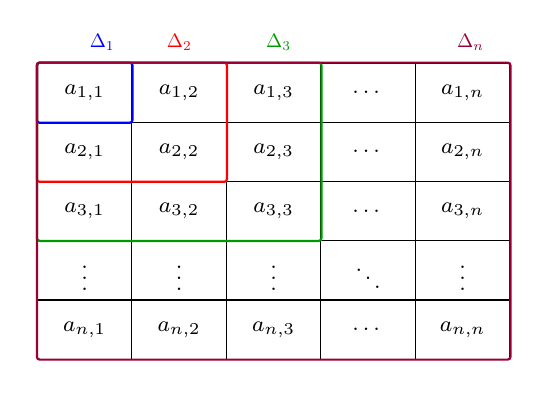
\begin{tikzpicture}[
        coeff/.style={draw, minimum width=1.2cm, minimum height=0.75cm, anchor=center, font=\footnotesize},
        zerocoeff/.style={minimum width=1.2cm, minimum height=0.75cm, anchor=center, font=\footnotesize}
    ]
        \matrix[matrix of nodes, 
                nodes={coeff}, 
                ampersand replacement=\&, 
                column sep=-\pgflinewidth,
                row sep=-\pgflinewidth
            ] (H) {
        $a_{1,1}$ \& $a_{1,2}$ \& $a_{1,3}$ \& $\dots$ \& $a_{1,n}$ \\
        $a_{2,1}$ \& $a_{2,2}$ \& $a_{2,3}$ \& $\dots$ \& $a_{2,n}$ \\
        $a_{3,1}$ \& $a_{3,2}$ \& $a_{3,3}$ \& $\dots$ \& $a_{3,n}$ \\
        $\vdots$  \& $\vdots$  \& $\vdots$  \& $\ddots$ \& $\vdots$  \\
        $a_{n,1}$ \& $a_{n,2}$ \& $a_{n,3}$ \& $\dots$ \& $a_{n,n}$ \\
        };

        \draw[blue, thick, rounded corners=1pt] (H-1-1.north west) rectangle (H-1-1.south east);
        \node at (H-1-1.north east) [above left, blue, scale=0.7, xshift=-2mm, yshift=1mm] {$\Delta_1$};
        \node at (H-1-1.north east) [above left, red, scale=0.7, xshift=12mm, yshift=1mm] {$\Delta_2$};
        \node at (H-1-1.north east) [above left, green!60!black, scale=0.7, xshift=30mm, yshift=1mm] {$\Delta_3$};
        \node at (H-1-1.north east) [above left, purple!80!black, scale=0.7, xshift=65mm, yshift=1mm] {$\Delta_n$};

        \draw[red, thick, rounded corners=1pt] (H-1-1.north west) rectangle (H-2-2.south east);
        \draw[green!60!black, thick, rounded corners=1pt] (H-1-1.north west) rectangle (H-3-3.south east);
        \draw[purple!80!black, thick, rounded corners=1pt] (H-1-1.north west) rectangle (H-5-5.south east);

    \end{tikzpicture}
    \captionof{figure}{Schematische Darstellung der Hauptminoren \(\Delta_k\).}
\end{center}
Die Vorzeichenfolge der Determinanten \(\det(\Delta_k)\) ist entscheidend:
\begin{itemize}
    \item \textbf{Positiv definit}: Alle Vorzeichen sind positiv. (\texttt{+, +, +, \dots})
    \item \textbf{Negativ definit}: Die Vorzeichen alternieren, beginnend mit negativ. (\texttt{-, +, -, +, \dots}) \newline
            \textbf{Achtung}: Die Vorzeichenfolgen \texttt{+, -, +, -, \dots} und \texttt{-, -, -, -, \dots} sind kontraintuitiv \textbf{NICHT} Negativ definit.
    \item \textbf{Indefinit}: Alle anderen Vorzeichenfolgen.
\end{itemize}
\textbf{Anmerkung:} Treten Nullen bei den Determinanten auf, kann dieses vereinfachte Kriterium nicht zuverlässig zwischen semidefinit und indefinit unterscheiden.

\subsection{Beispiel}
Untersuchung der Matrix \[ A = \begin{pmatrix} -2 & 1 & 0 \\ 1 & -2 & 1 \\ 0 & 1 & -2 \end{pmatrix} \]
\begin{itemize}
    \item \(\det(\Delta_1) = -2\)
    \item \(\det(\Delta_2) = \begin{vmatrix} -2 & 1 \\ 1 & -2 \end{vmatrix} = 3\)
    \item \(\det(\Delta_3) = \det(A) = -4\)
\end{itemize}
Die Vorzeichenfolge ist \texttt{-, +, -}. Die Matrix ist somit \textbf{negativ definit}.
	\chapter{Eigenwerte und Eigenvektoren}
Die Multiplikation einer quadratischen Matrix $A$ mit einem ihrer Eigenvektoren $\vec{v}$ resultiert in einem skalierten Vielfachen des selben Vektors. Der Skalierungsfaktor wird als Eigenwert $\lambda$ bezeichnet.

\section{Eigenwerte Berechnen}
Die Eigenwerte $\lambda$ einer Matrix $A$ werden durch das Nullsetzen der Determinante von $(A - \lambda I)$ ermittelt.
\[
    \det(A - \lambda I) = 0
\]
Die resultierenden Nullstellen für $\lambda$ sind die Eigenwerte der Matrix.

\section{Eigenvektoren Berechnen}
Für jeden Eigenwert $\lambda_i$ wird der zugehörige Eigenvektor $\vec{x}$ durch das Lösen des folgenden linearen Gleichungssystems gefunden:
\[
    (A - \lambda_i I) \vec{x} = \vec{0}
\]
Der Lösungsraum (Spannraum) dieses Systems stellt die Menge der Eigenvektoren zum jeweiligen Eigenwert $\lambda_i$ dar.

	\part{Bonusteste}
	\chapter{Bonustest 1 - Rechnen mit Vektoren}

\section{Frage 1}
Wie viele verschiedene Vektoren sind auf diesem Bild zu sehen?

In dieser Aufgabe geht es im wesentlichen darum, die \textbf{verschiedenen} Pfeile zu zählen. Es ist 
hilfreich, die Vektoren in dem Graphen so zu verschieben, dass gleiche Vektoren beieinander sind. So 
muss nur noch die Anzahl der Cluster gezählt werden.

\makebox[0.5\textwidth]{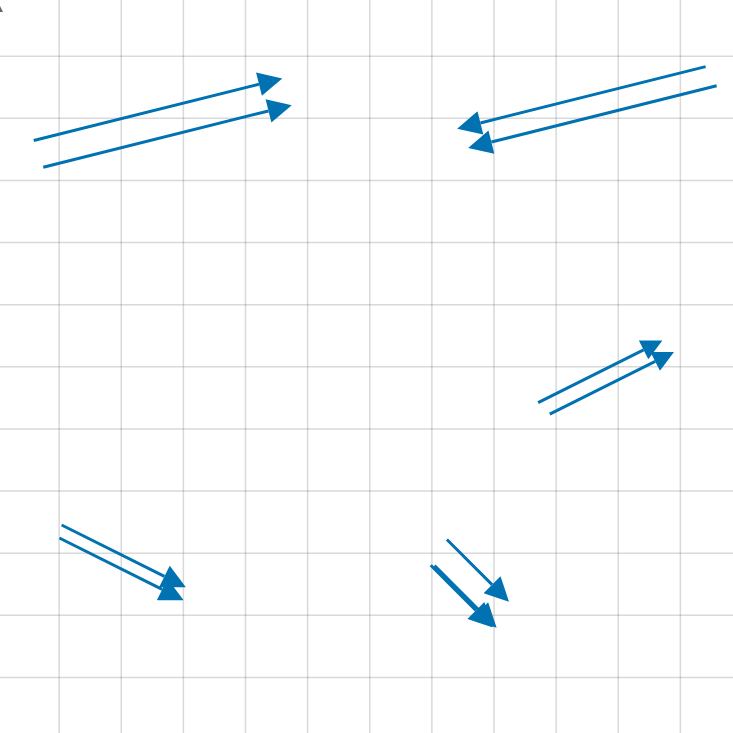
\includegraphics[width=0.5\textwidth]{bonus_tests/unique_vectors.png}}

Hier gibt es \textbf{5} verschiedene Vektoren.

\section{Frage 2}
In der folgenden Abbildung sind verschiedene Vektoren dargestellt. Ein Kästchen entspricht einer Längeneinheit.
Geben Sie die verschiedenen Vektoren, die im Bild zu sehen sind, als Liste in eckigen Klammern an. 
Die Einträge dieser Liste sind dabei die verschiedenen Vektoren dargestellt als Paare von Zahlen in eckigen Klammern. 
Ihre Antwort sollte also ein Ausdruck der Form [[1,3],[-2,0],[1,1]] oder [[0,3],[1,-1],[-1,1],[4,2]] etc. sein. 

Hier ist es auch wieder Sinnvoll, die Vektoren zu sortieren. Dann müssen die Vektoren nur noch abgelesen werden.
Die Vektoren werden über [x, y] benannt, wobei x der weg ist, den der Vektor nach rechts "geht" und y die höhe 
des Vektors ist.

\makebox[0.5\textwidth]{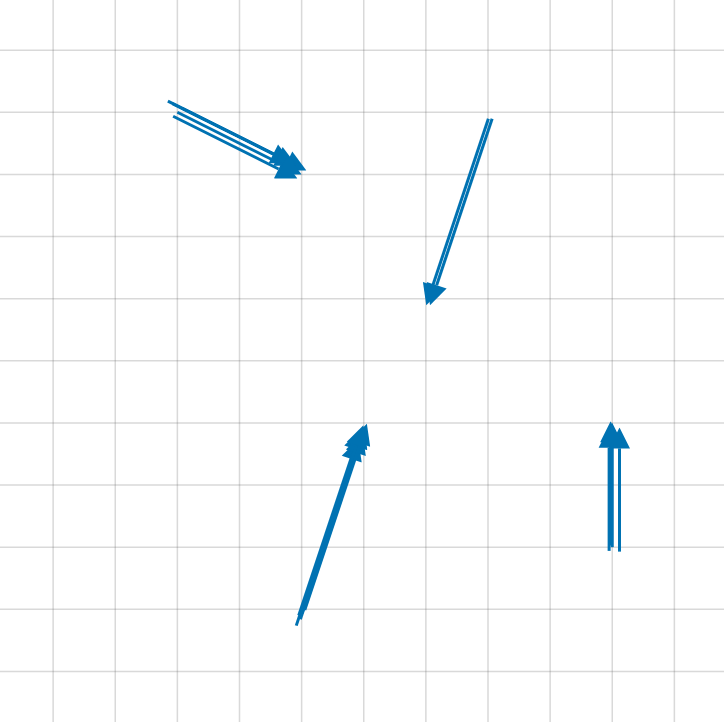
\includegraphics[width=0.5\textwidth]{bonus_tests/vector_lengths.png}}

Hier befinden sich in der Abbildung die Vektoren [[1, 3], [0, 2], [2, -1], [-1, -3]]

\section{Frage 3}
Gegeben sind im $\mathbb{R}^3$ die beiden Vektoren $\vec{u}$ und $\vec{v}$ in Komponentendarstellung,
wobei $B = (\vec{e_1}, \vec{e_2}, \vec{e_3})$ die Standardbasis des $\mathbb{R}^3$ ist.

\subsection{a}
Geben Sie die Vektoren $\vec{u}$ und $\vec{v}$ in Koordinatendarstellung an.

\subsubsection{I}
Es ist $\vec{u} = \frac{3\vec{e_3}}{2} + 2\vec{e_2} + 3\vec{e_1}$

Hier muss der Vektor berechnet werden. Da die Vektoren $\vec{e_1}, \vec{e_2}, \vec{e_3}$ die standardvektoren sind,
ist deren Wert bekannt $\left(\vec{e_1} = \begin{pmatrix}
    1 \\ 0 \\ 0
\end{pmatrix}, \vec{e_2} = \begin{pmatrix}
    0 \\ 1 \\ 0
\end{pmatrix}, \vec{e_3} = \begin{pmatrix}
    0 \\ 0 \\ 1
\end{pmatrix}\right)$. 

Bevor das Ergebnis berechnet wird, sollte noch der Bruch aufgelöst werden: 
\begin{align*}
    \frac{3\vec{e_3}}{2} = \frac{3 \cdot \vec{e_3}}{2 \cdot 1} = \frac{3}{2} \cdot \frac{\vec{e_3}}{1} = \frac{3}{2}\vec{e_3}
\end{align*}

Jetzt können die Einheitsvektoren einfach eingesetzt werden

\begin{align*}
    \frac{3}{2} \cdot \begin{pmatrix} 0 \\ 0 \\ 1 \end{pmatrix} + 2 \cdot \begin{pmatrix} 0 \\ 1 \\ 0 \end{pmatrix} + 3 \cdot \begin{pmatrix} 1 \\ 0 \\ 0 \end{pmatrix} \\
    =  \begin{pmatrix}
        \frac{3}{2} \cdot 0 \\ \frac{3}{2} \cdot 0 \\ \frac{3}{2} \cdot 1
    \end{pmatrix} + \begin{pmatrix}
        2 \cdot 0 \\ 2 \cdot 1 \\ 2 \cdot 0
    \end{pmatrix} + \begin{pmatrix}
        3 \cdot 1 \\ 3 \cdot 0 \\ 3 \cdot 0
    \end{pmatrix} \\\pagebreak[2]
    = \begin{pmatrix}
        0 \\ 0 \\ \frac{3}{2}
    \end{pmatrix} + \begin{pmatrix}
        0 \\ 2 \\ 0
    \end{pmatrix} + \begin{pmatrix}
        3 \\ 0 \\ 0
    \end{pmatrix} \\\pagebreak[2]
    = \begin{pmatrix}
        3 \\ 2 \\ \frac{3}{2}
    \end{pmatrix}
\end{align*}

Der Vektor $\vec{u}$ ist also $\begin{pmatrix}
    3 \\ 2 \\ \frac{3}{2}
\end{pmatrix}$.

\subsubsection{II}
es ist $\vec{v} = 2\vec{e_3} + 2\vec{e_2}$.

Hier können wieder die Einheitsvektoren eingesetzt werden.

\begin{align*}
    2 \cdot \begin{pmatrix}
        0 \\ 0 \\ 1
    \end{pmatrix} + 2 \cdot \begin{pmatrix}
        0 \\ 1 \\ 0
    \end{pmatrix} \\
    = \begin{pmatrix}
        2 \cdot 0 \\ 2 \cdot 0 \\ 2 \cdot 1
    \end{pmatrix} + \begin{pmatrix}
        2 \cdot 0 \\ 2 \cdot 1 \\ 2 \cdot 0
    \end{pmatrix} \\
    = \begin{pmatrix}
        0 \\ 0 \\ 2
    \end{pmatrix} + \begin{pmatrix}
        0 \\ 2 \\ 0
    \end{pmatrix} \\
    = \begin{pmatrix}
        0 \\ 2 \\ 2
    \end{pmatrix}
\end{align*}

\subsection{b}
Berechnen Sie für die Vektoren $\vec{u}$ und $\vec{v}$ aus Teilaufgabe a folgende Größen.
Geben Sie die Lösung exakt, also nicht näherungsweise an.

\subsubsection{I}
Es ist $\vec{u} - 2\vec{v}$

\begin{align*}
    \begin{pmatrix}
        3 \\ 2 \\ \frac{3}{2}
    \end{pmatrix} - 2 \cdot \begin{pmatrix}
        0 \\ 2 \\ 2
    \end{pmatrix} \\
    = \begin{pmatrix}
        3 \\ 2 \\ \frac{3}{2}
    \end{pmatrix} - \begin{pmatrix}
        0 \\ 4 \\ 4
    \end{pmatrix} \\
    = \begin{pmatrix}
        3 - 0\\ 2 - 4 \\ \frac{3}{2} - 4
    \end{pmatrix} \\
    = \begin{pmatrix}
        3 \\ -2 \\ -\frac{5}{2}
    \end{pmatrix}
\end{align*}

\subsubsection{II}
Es ist $\left|3\vec{u} + 3\vec{v}\right|$

Die Betragsstriche meinen hier, dass die Länge des Vektors berechnet werden soll. 
Diese kann über die Formel $\sqrt{v_1^2 + v_2^2 + \dots + v_n^2}$ berechnet werden.
Es muss also zunächst der resultierende Vektor von $3\vec{u} + 3\vec{v}$ berechnet werden und 
von diesen Vektor muss dann die Länge bestimmt werden.

\begin{align*}
    \left|3 \cdot \begin{pmatrix}
        3 \\ 2 \\ \frac{3}{2}
    \end{pmatrix} + 3 \cdot \begin{pmatrix}
        0 \\ 2 \\ 2
    \end{pmatrix}\right| \\
    = \left|\begin{pmatrix}
        3 \cdot 3 \\ 3 \cdot 2 \\ 3 \cdot \frac{3}{2}
    \end{pmatrix} + \begin{pmatrix}
        3 \cdot 0 \\ 3 \cdot 2 \\ 3 \cdot 2
    \end{pmatrix}\right| \\
    = \left|\begin{pmatrix}
        9 \\ 6 \\ \frac{9}{2}
    \end{pmatrix} + \begin{pmatrix}
        0 \\ 6 \\ 6
    \end{pmatrix}\right| \\
    = \left|\begin{pmatrix}
        9 \\ 12 \\ \frac{21}{2}
    \end{pmatrix}\right| \\
    = \sqrt{9^2 + 12^2 + \frac{21}{2}^2} \\
    = \sqrt{\frac{1341}{2}}
\end{align*}

\subsubsection{III}
Es ist $\left\langle\vec{u}, \vec{v}\right\rangle$

Hier soll das Skalarprodukt berechnet werden. Das Skalarprodukt $\left\langle\vec{a}, \vec{b}\right\rangle$
berechnet sich aus $a_1 \cdot b_1 + a_2 + b_2 + \dots + a_n + b_n$

\begin{align*}
    \left\langle \begin{pmatrix}
        3 \\ 2 \\ \frac{3}{2}
    \end{pmatrix}, \begin{pmatrix}
        0 \\ 2 \\ 2
    \end{pmatrix}\right\rangle \\
    = 3 \cdot 0 + 2 \cdot 2 + \frac{3}{2} \cdot 2 \\
    = 0 + 4 + 3 \\
    = 7
\end{align*}

\subsubsection{IV}
Es ist $\vec{u} \times \vec{v}$

Hier soll das Kreuzprodukt berechnet werden. Das Kreuzprodukt zweier Vektoren $\vec{a}, \vec{b}$ der länge 3 lässt sich 
über $\begin{pmatrix}a_2b_3 - a_3b_2 \\ a_3b_1 - a_1b_3 \\ a_1b_2 - a_2b_1 \end{pmatrix}$

\begin{align*}
    \begin{pmatrix}
        3 \\ 2 \\ \frac{3}{2}
    \end{pmatrix} \times \begin{pmatrix}
        0 \\ 2 \\2
    \end{pmatrix} \\
    = \begin{pmatrix}
        2 \cdot 2 - \frac{3}{2} \cdot 2 \\ \frac{3}{2} \cdot 0 - 3 \cdot 2 \\ 3 \cdot 2 - 2 \cdot 0
    \end{pmatrix} \\
    = \begin{pmatrix}
        4 - 3 \\ 0 - 6 \\ 6 - 0
    \end{pmatrix} \\
    = \begin{pmatrix}
        1 \\ -6 \\ 6
    \end{pmatrix}
\end{align*}

\section{Frage 4}
In welchem der folgenden Bilder ist das Skalarprodukt $\left\langle \vec{a}, \vec{b} \right\rangle$ negativ?

Das Skalarprodukt zweier Vektoren ist negativ, wenn der Winkel zwischen den Vektoren größer als 90° beträgt.

\subsection*{Herleitung: Vorzeichen des Skalarprodukts}
Das Skalarprodukt zweier Vektoren $\vec{a}$ und $\vec{b}$ ist fundamental durch ihre Beträge und den von ihnen 
eingeschlossenen Winkel $\theta$ definiert:
$$ \left\langle \vec{a}, \vec{b} \right\rangle = |\vec{a}| \cdot |\vec{b}| \cdot \cos(\theta) $$
Hierbei sind $|\vec{a}|$ und $|\vec{b}|$ die Längen der Vektoren. Der Winkel $\theta$ ist der 
kleinste Winkel zwischen $\vec{a}$ und $\vec{b}$, sodass $0^\circ \le \theta \le 180^\circ$.

\subsubsection*{Die Rolle des Kosinus}
Die Beträge $|\vec{a}|$ und $|\vec{b}|$ sind per Definition stets nicht-negativ. Wenn wir annehmen, 
dass weder $\vec{a}$ noch $\vec{b}$ der Nullvektor ist (d.h. $|\vec{a}| > 0$ und $|\vec{b}| > 0$), dann 
sind ihre Beträge positive Zahlen.
Das Produkt zweier positiver Zahlen ($|\vec{a}| \cdot |\vec{b}|$) ist ebenfalls positiv.
Folglich hängt das Vorzeichen des gesamten Skalarprodukts $\left\langle \vec{a}, \vec{b} \right\rangle$ 
ausschließlich vom Vorzeichen des Terms $\cos(\theta)$ ab:
$$ \text{Vorzeichen}(\left\langle \vec{a}, \vec{b} \right\rangle) = \text{Vorzeichen}(\cos(\theta)) $$

\subsubsection*{Verhalten von $\cos(\theta)$ im relevanten Winkelbereich}
Betrachten wir das Vorzeichen von $\cos(\theta)$ für die möglichen Werte des Winkels $\theta$ zwischen zwei Vektoren:
\begin{itemize}
    \item \textbf{Spitzer Winkel:} $0^\circ \le \theta < 90^\circ$
    
    Für Winkel in diesem Bereich ist der Kosinus positiv: $\cos(\theta) > 0$.
    Das Skalarprodukt ist somit:
    $$ \left\langle \vec{a}, \vec{b} \right\rangle = \underbrace{|\vec{a}| \cdot |\vec{b}|}_{\text{positiv}} 
    \cdot \underbrace{\cos(\theta)}_{\text{positiv}} \quad \implies \quad \left\langle \vec{a}, \vec{b} 
    \right\rangle > 0 $$
    
    \item \textbf{Rechter Winkel:} $\theta = 90^\circ$
    
    Für einen rechten Winkel ist der Kosinus Null: $\cos(90^\circ) = 0$.
    Das Skalarprodukt ist somit:
    $$ \left\langle \vec{a}, \vec{b} \right\rangle = |\vec{a}| \cdot |\vec{b}| \cdot 
    \underbrace{\cos(90^\circ)}_{0} \quad \implies \quad \left\langle \vec{a}, \vec{b} \right\rangle = 0 $$
    In diesem Fall stehen die Vektoren orthogonal (senkrecht) aufeinander.
    
    \item \textbf{Stumpfer Winkel:} $90^\circ < \theta \le 180^\circ$
    
    Für Winkel in diesem Bereich ist der Kosinus negativ: $\cos(\theta) < 0$.
    Das Skalarprodukt ist somit:
    $$ \left\langle \vec{a}, \vec{b} \right\rangle = \underbrace{|\vec{a}| \cdot |\vec{b}|}_{\text{positiv}} 
    \cdot \underbrace{\cos(\theta)}_{\text{negativ}} \quad \implies \quad \left\langle \vec{a}, \vec{b} 
    \right\rangle < 0 $$
\end{itemize}

\subsubsection*{Schlussfolgerung aus der Herleitung}
Das Skalarprodukt $\left\langle \vec{a}, \vec{b} \right\rangle$ ist \textbf{genau dann negativ}, wenn der 
Kosinus des von den Vektoren eingeschlossenen Winkels $\theta$ negativ ist. Dies ist der Fall, wenn der 
Winkel $\theta$ ein stumpfer Winkel ist, also $90^\circ < \theta \le 180^\circ$.

\section{Aufgabe 5}

Gegeben sind zwei $\mathbb{R}^3$-Vektoren

\[
\vec{a} = \begin{pmatrix}
    -\frac{3}{2} \\
    \frac{8}{3} \\
    1
\end{pmatrix} \quad \vec{b} = \begin{pmatrix}
    1 \\ 0 \\ \frac{8}{3}
\end{pmatrix}
\]

Bestimmen Sie den Winkel zwischen $a$ und $b$ und runden diesen auf zwei Dezimalstellen genau in Grad und Bogenmaß.

\subsection{a}

Der Winkel zwischen zwei Vektoren kann berechnet werden, über $\cos(\theta) = \frac{\left\langle \vec{a}, \vec{b} \right\rangle}{\left|\vec{a}\right| \cdot \left|\vec{b}\right|}$. Hier müssen ganz einfach die Vektoren eingesetzt werden

\begin{align*}
    \cos(\theta) = \frac{\left\langle \vec{a}, \vec{b} \right\rangle}{\left|\vec{a}\right| \cdot \left|\vec{b}\right|} \\\\
    \left\langle \vec{a}, \vec{b} \right\rangle = -\frac{3}{2} \cdot 1 + \frac{8}{3} \cdot 0 + 1 \cdot \frac{8}{3} \\
    = -\frac{3}{2} + \frac{8}{3} \\
    = \frac{7}{6} \\\\
    \left|a\right| = \sqrt{{(-\frac{3}{2})}^2 + \frac{8}{3}^2 + 1^2} \\
    = \sqrt{{\frac{9}{4}} + \frac{64}{9} + 1}
    = \sqrt{\frac{373}{36}} \\\\
    \left|b\right| = \sqrt{1^2 + 0^2 + \frac{8}{3}^2} \\
    = \sqrt{1 + 0 + \frac{64}{9}}
    = \sqrt{\frac{73}{9}} \\\\
    \cos(\theta) = \frac{\frac{7}{6}}{\sqrt{\frac{373}{36}} \cdot \sqrt{\frac{73}{9}}} = \frac{21 \sqrt{27229}}{27229} \\
    \arccos\left(\frac{21 \sqrt{27229}}{27229}\right) \approx 1.44 rad \\
    \arccos\left(\frac{21 \sqrt{27229}}{27229}\right) \cdot \frac{180}{\pi} \approx 82.71^\circ
\end{align*}

Der Winekl zwischen den gegebenen Vektoren beträgt in Gradmaß $\theta_{grad}$ = $82.71$.

\subsection{b}

Der Winkel zwischen den gegebenen Vektoren beträgt in Bogenmaß $\theta_{Bogen}$ = $1.44$.

\section{Aufgabe 6}

Gegeben sind die zwei Ortsvektoren
\[
    \vec{u} = \begin{pmatrix}
        5 \\ -1 \\ 4
    \end{pmatrix}, \quad \vec{v} = \begin{pmatrix}
        -1 \\ 0 \\ -2
    \end{pmatrix} \text{ der beiden Punkte } U \text{ und } V\text{.}
\]

\subsection{a}

Wie in der folgenden Abbildung dargestellt, unterteilen die Punkte $U$ und $V$ die Strecke von Punkt $X$ zu Punkt $Y$ in drei gleich lange Teile.

\begin{center}
\begin{tikzpicture}[
    punkt/.style={circle, fill, inner sep=1.5pt},
  ]

  \coordinate (x) at (0, 0);
  \coordinate (y) at (7, 1.5);

  \draw[cyan, line width=1.2pt] (x) -- (y);

  \node[punkt, cyan, label=below left:$X$] at (x) {};
  \node[punkt, cyan, label=above right:$Y$] at (y) {};

  \path (x) -- (y) coordinate[pos=1/3] (u) coordinate[pos=2/3] (v);

  \draw[black, line width=1.2pt] (u) -- (v);

  \node[punkt, black, label=above:$U$] at (u) {};
  \node[punkt, black, label=above:$V$] at (v) {};
\end{tikzpicture}
\end{center}

Bestimmen Sie die Ortsvektoren $\vec{x}$ und $\vec{y}$ der Punkte $X$ und $Y$.

\subsubsection{Lösung}
Der Verbindungsvektor von Punkt $U$ nach Punkt $V$ lässt sich aus den zugehörigen Ortsvektoren $\vec{u}$ und $\vec{v}$ berechnen:
\begin{align*}
    \vec{UV} &= \vec{v} - \vec{u} \\
    &= \begin{pmatrix}
        -1 \\ 0 \\ -2
    \end{pmatrix} - \begin{pmatrix}
        5 \\ -1 \\ 4
    \end{pmatrix} \\
    &= \begin{pmatrix}
        -6 \\ 1 \\ -6
    \end{pmatrix}
\end{align*}
Da die Strecke in drei gleich lange Teile unterteilt ist, gilt $\vec{XU} = \vec{UV} = \vec{VY}$.
\newline
\newline
Der Ortsvektor $\vec{x}$ des Punktes $X$ kann somit durch Subtraktion des Vektors $\vec{UV}$ vom Ortsvektor $\vec{u}$ bestimmt werden:
\begin{align*}
    \vec{x} &= \vec{u} - \vec{UV} \\
    &= \begin{pmatrix}
        5 \\ -1 \\ 4
    \end{pmatrix} - \begin{pmatrix}
        -6 \\ 1 \\ -6
    \end{pmatrix} \\
    &= \begin{pmatrix}
        11 \\ -2 \\ 10
    \end{pmatrix}
\end{align*}
Analog ergibt sich der Ortsvektor $\vec{y}$ des Punktes $Y$ aus der Addition des Vektors $\vec{UV}$ zum Ortsvektor $\vec{v}$:
\begin{align*}
    \vec{y} &= \vec{v} + \vec{UV} \\
    &= \begin{pmatrix}
        -1 \\ 0 \\ -2
    \end{pmatrix} + \begin{pmatrix}
        -6 \\ 1 \\ -6
    \end{pmatrix} \\
    &= \begin{pmatrix}
        -7 \\ 1 \\ -8
    \end{pmatrix}
\end{align*}

\subsection{b}

Bestimmen Sie die Ortsvektoren $\vec{x}$ und $\vec{y}$ als Linearkombination von $\vec{u}$ und $\vec{v}$.

\subsubsection*{Lösung}
Aus Teil a sind die Beziehungen $\vec{x} = \vec{u} - \vec{UV}$ und $\vec{y} = \vec{v} + \vec{UV}$ bekannt, sowie $\vec{UV} = \vec{v} - \vec{u}$. Durch Einsetzen von $\vec{UV}$ lässt sich $\vec{x}$ als Linearkombination von $\vec{u}$ und $\vec{v}$ darstellen:
\begin{align*}
    \vec{x} &= \vec{u} - (\vec{v} - \vec{u}) \\
    &= \vec{u} - \vec{v} + \vec{u} \\
    &= 2\vec{u} - \vec{v}
\end{align*}
Ebenso für $\vec{y}$:
\begin{align*}
    \vec{y} &= \vec{v} + (\vec{v} - \vec{u}) \\
    &= \vec{v} + \vec{v} - \vec{u} \\
    &= 2\vec{v} - \vec{u}
\end{align*}
Die gesuchten Linearkombinationen lauten somit:
\[
    \vec{x} = 2\vec{u} - \vec{v} \quad \text{und} \quad \vec{y} = - \vec{u} + 2\vec{v}
\]

\section{Aufgabe 7}

Auf einem Billardtisch befinden sich eine blaue und eine weiße Kugel. Die weiße Kugel und die blaue Kugel haben beide einen Durchmesser \(d = 57.2\,\text{mm}\). In der folgenden Abbildung ist der Billardtisch dargestellt. Der Punkt \(A\) bezeichnet den Mittelpunkt der weißen Kugel und der Punkt \(B\) den Mittelpunkt der blauen Kugel. Die Punkte liegen jeweilts auf einem Gitterpunkt des quadratischen Rasters, wobei ein Kästchen eine skalierung von \(1\,\text{dm}\) hat. Die obere rechte Tasche des Billarftisches wird mit \(C\) und die untere rechte Tasche mit \(D\) bezeichnet.

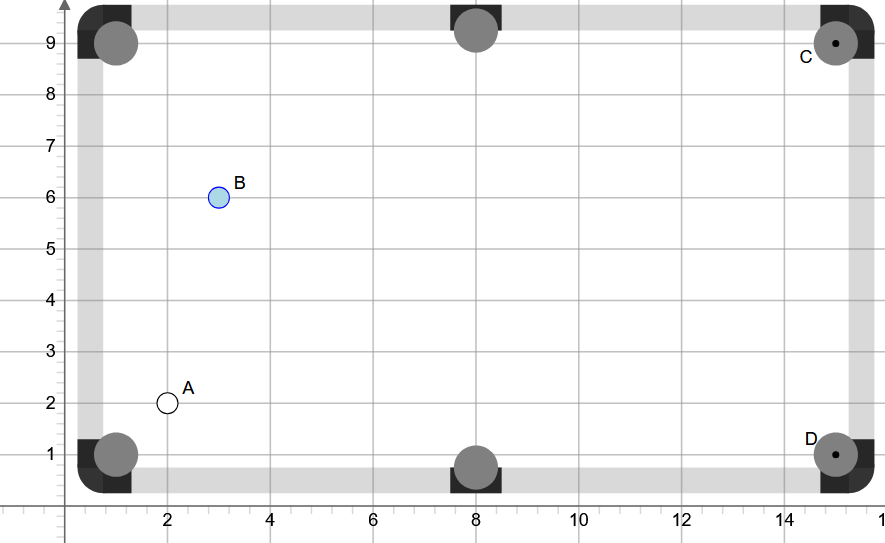
\includegraphics[width=\textwidth]{bonus_tests/pool.png}

Hier ist die Kugel B bei \(\begin{pmatrix} 3 \\ 6 \end{pmatrix}\) und die Kugel A bei \(\begin{pmatrix} 2 \\ 2 \end{pmatrix}\).

Die weiße Kugel wird so gespielt, dass die blaue Kugel danach direkt zu Punkt \(C\) rollt. Die folgende Abbildung zeigt die weiße und blaue Kugel beim Stoß. Dabei ist \(A'\) die Position der weißen Kugel, wenn diese auf die blaue Kugel trifft. Der Impuls wird hierbei entlang der Linie \(A'B\) übertragen.

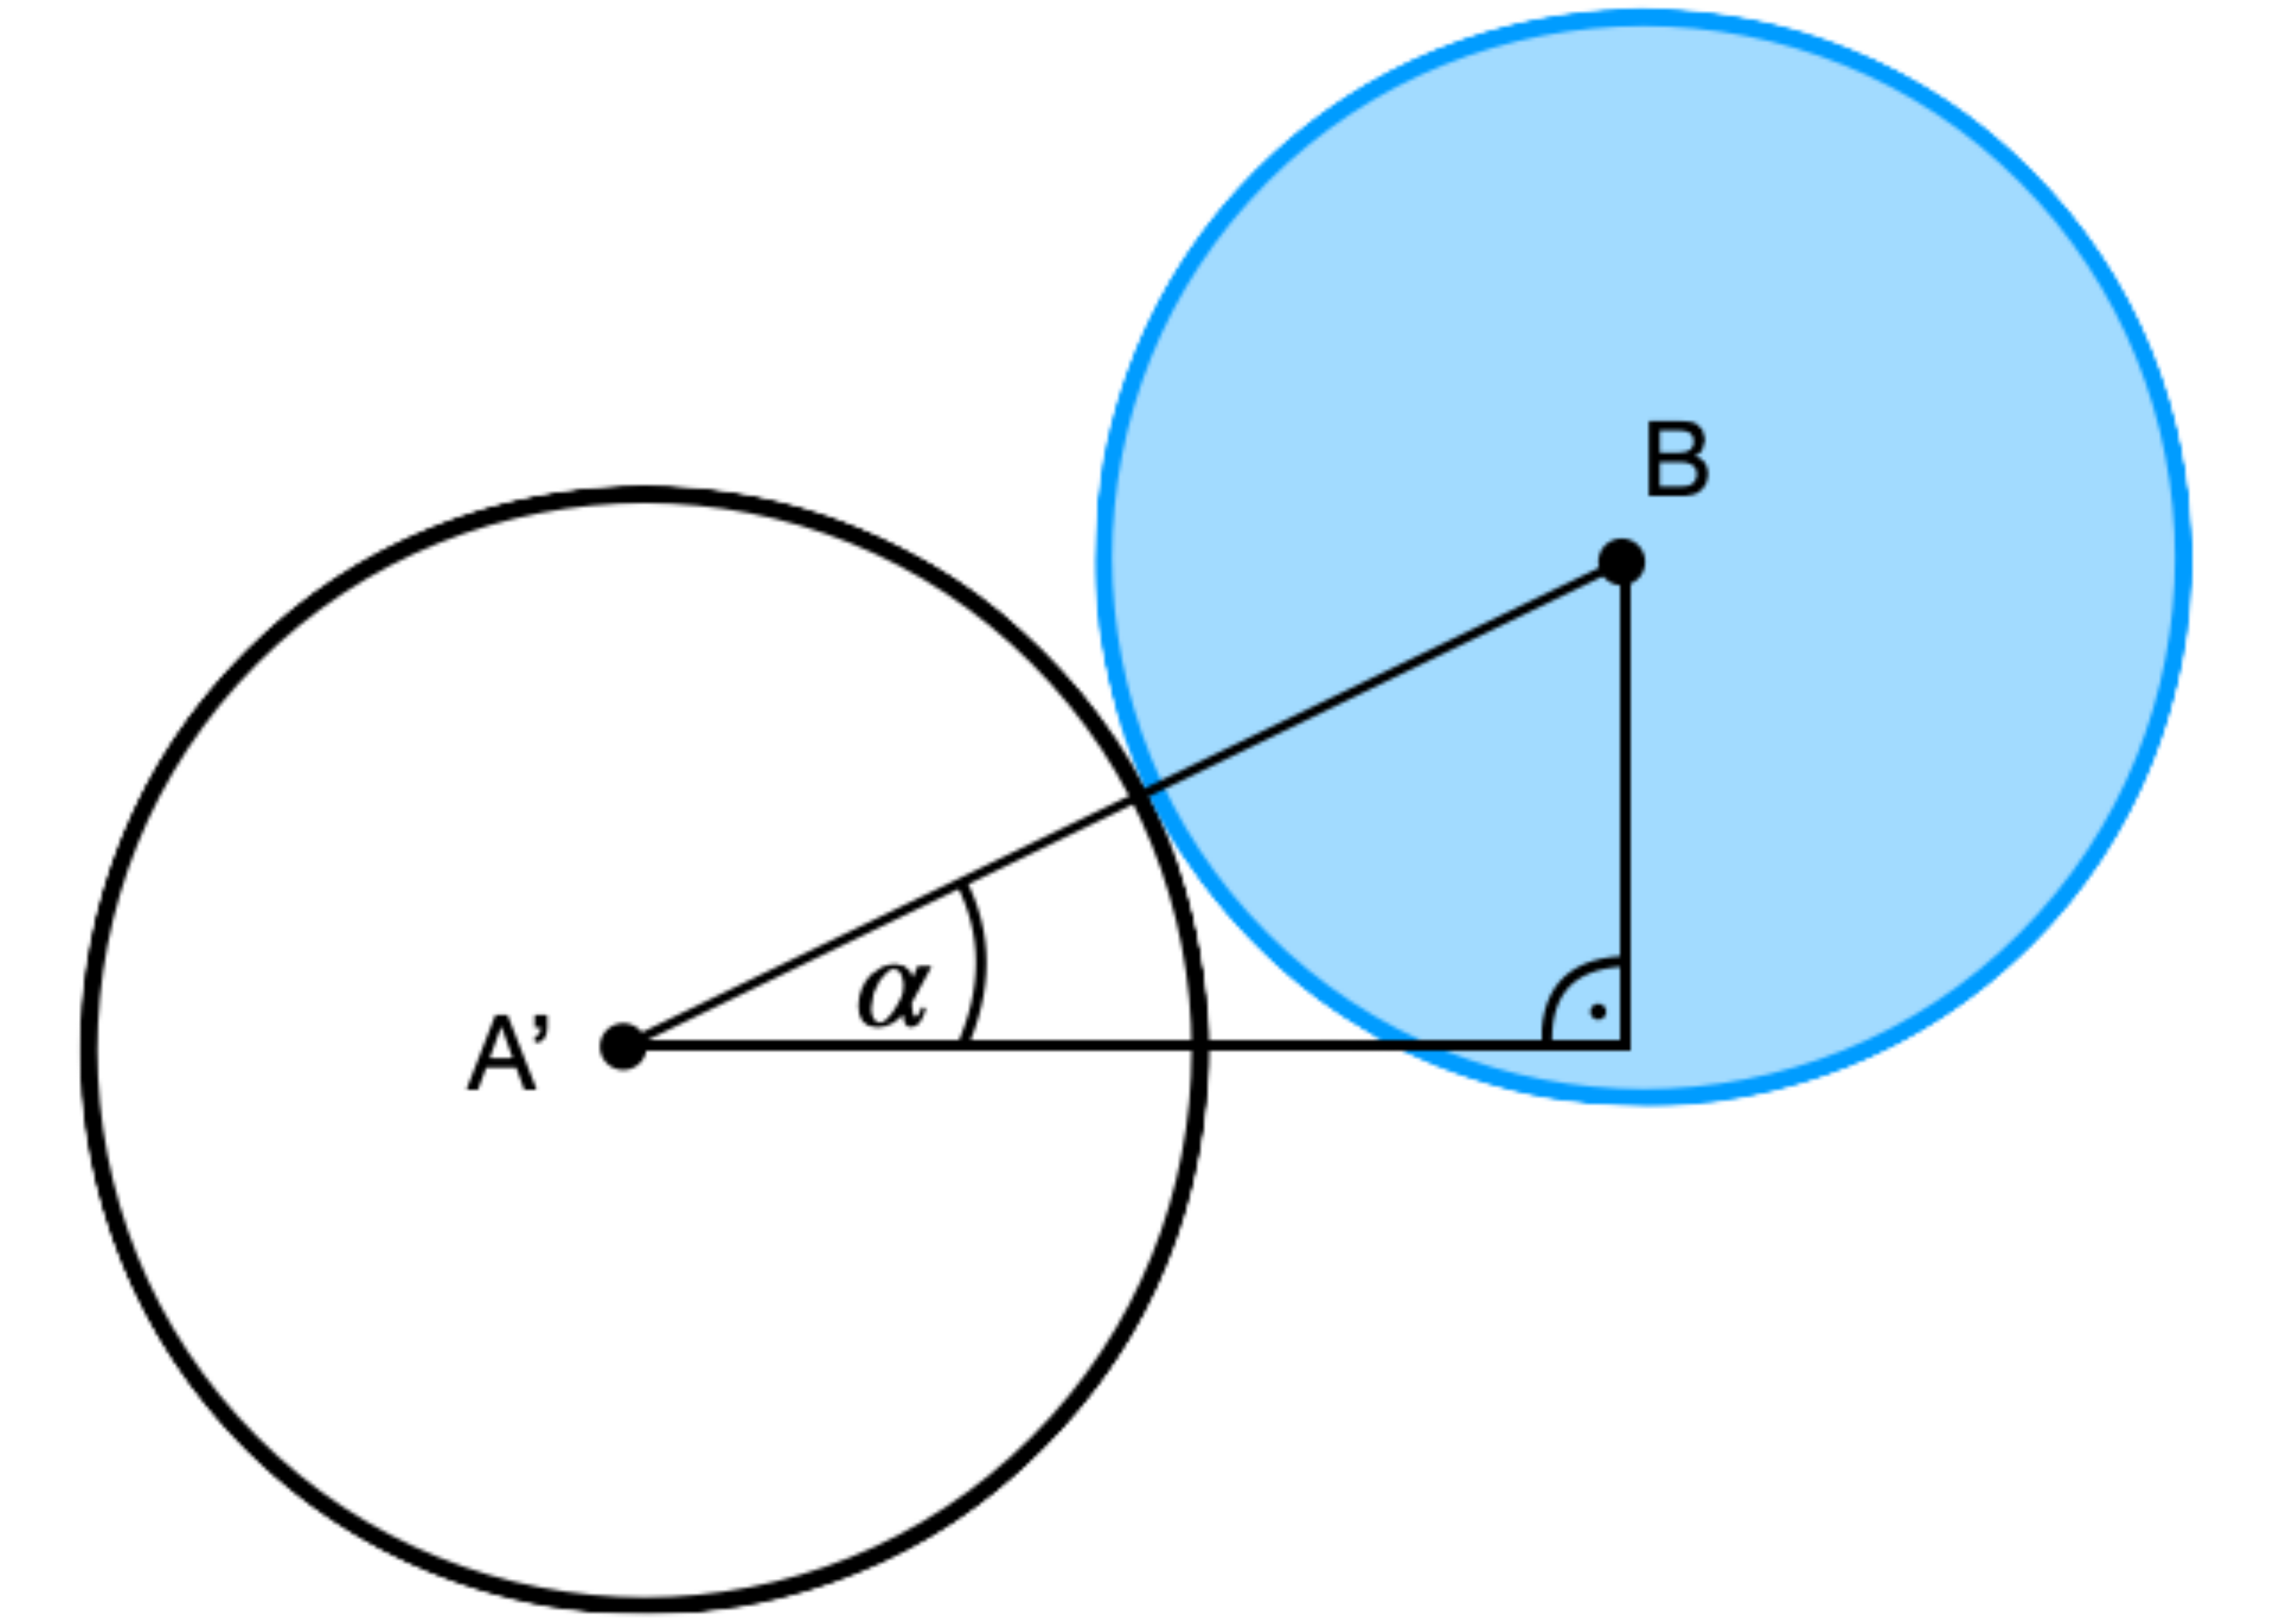
\includegraphics[width=\textwidth]{bonus_tests/pool2.png}

\subsection{a}

Berechnen Sie den Winkel \(\alpha\), unter dem die weiße Kugel die blaue Kugel treffen muss, damit die blaue Kugel direkt in Loch \(C\) trifft. Geben Sie den Winkel in Gradmaß und auf zwei Dezimalstellen genau ein.

Der Richtungsvektor der blauen Kugel ist \(\vec{BC}\).
\[
\vec{BC} = \vec{C} - \vec{B} = \begin{pmatrix} 15 \\ 9 \end{pmatrix} - \begin{pmatrix} 3 \\ 6 \end{pmatrix} = \begin{pmatrix} 12 \\ 3 \end{pmatrix}
\]
Der Winkel \(\theta\) dieses Vektors zur x-Achse \(\begin{pmatrix} 1 \\ 0 \end{pmatrix}\) ist:
\begin{align*}
    \cos(\theta) &= \frac{\begin{pmatrix} 12 \\ 3 \end{pmatrix} \cdot \begin{pmatrix} 1 \\ 0 \end{pmatrix}}{|\begin{pmatrix} 12 \\ 3 \end{pmatrix}| \cdot |\begin{pmatrix} 1 \\ 0 \end{pmatrix}|} = \frac{12}{\sqrt{12^2 + 3^2} \cdot \sqrt{1^2}} = \frac{12}{\sqrt{153}} \\
    \theta &= \arccos\left(\frac{12}{\sqrt{153}}\right) \approx 14.04^\circ
\end{align*}

\subsection{b}
Berechnen Sie den Vektor \(\vec{A'B}\) in dm und auf zwei Dezimalstellen genau.

Der Vektor \(\vec{A'B}\) verläuft vom Zentrum der weißen Kugel (\(A'\)) zum Zentrum der blauen Kugel (\(B\)) im Moment des Stoßes. Er hat die Richtung von \(\vec{BC}\) und die Länge des Kugeldurchmessers \(d = 0.572\,\text{dm}\).
\begin{align*}
    \vec{A'B} &= d \cdot \frac{\vec{BC}}{|\vec{BC}|} = 0.572 \cdot \frac{1}{\sqrt{153}}\begin{pmatrix} 12 \\ 3 \end{pmatrix} \\
    &\approx 0.572 \cdot \begin{pmatrix} 0.9701 \\ 0.2425 \end{pmatrix} \approx \begin{pmatrix} 0.55 \\ 0.14 \end{pmatrix}
\end{align*}

\subsection{c}

Bestimmen Sie den Vektor \(\vec{AA'}\), in dessen Richtung die weiße Kugel gespielt wird, in dm und auf zwei Dezimalstellen genau.

Zuerst wird die Position von \(A'\) bestimmt: \(\vec{A'} = \vec{B} - \vec{A'B}\).
\begin{align*}
    \vec{A'} &\approx \begin{pmatrix} 3 \\ 6 \end{pmatrix} - \begin{pmatrix} 0.55 \\ 0.14 \end{pmatrix} = \begin{pmatrix} 2.45 \\ 5.86 \end{pmatrix}
\end{align*}
Der Vektor der Stoßrichtung \(\vec{AA'}\) ist dann \(\vec{A'} - \vec{A}\).
\begin{align*}
    \vec{AA'} &\approx \begin{pmatrix} 2.45 \\ 5.86 \end{pmatrix} - \begin{pmatrix} 2 \\ 2 \end{pmatrix} = \begin{pmatrix} 0.45 \\ 3.86 \end{pmatrix}
\end{align*}

\subsection{d}
Berechnen Sie den Winkel \(\beta\) zwischen dem Stoßvektor \(\vec{AA'}\) und der Horizontalen.

Der gesuchte Winkel \(\beta\) ist der Winkel zwischen dem Stoßvektor \(\vec{AA'}\) und der horizontalen Achse.
\begin{align*}
    \cos(\beta) &= \frac{\vec{AA'} \cdot \begin{pmatrix} 1 \\ 0 \end{pmatrix}}{|\vec{AA'}| \cdot |\begin{pmatrix} 1 \\ 0 \end{pmatrix}|} \\
    \vec{AA'} \cdot \begin{pmatrix} 1 \\ 0 \end{pmatrix} &\approx 0.45 \cdot 1 + 3.86 \cdot 0 = 0.45 \\
    |\vec{AA'}| &\approx \sqrt{0.45^2 + 3.86^2} = \sqrt{0.2025 + 14.8996} = \sqrt{15.1021} \approx 3.886 \\
    |\begin{pmatrix} 1 \\ 0 \end{pmatrix}| &= 1 \\
    \cos(\beta) &\approx \frac{0.45}{3.886 \cdot 1} \approx 0.1158 \\
    \beta &= \arccos(0.1158) \approx 83.35^\circ
\end{align*}
Der gesuchte Winkel beträgt also \(83.35^\circ\).

\section{Aufgabe 8}

Auf einem Körper, der den Punkt $O$ drehbar ist, wirkt eine am Punkt $R$ angreifende Kraft $\vec{F}$. Der vektor $\vec{r}$ ist der Ortsvektor von Punkt $O$ nach Punkt $R$. In der folgenden Abbildung ist der Körper dargestellt.

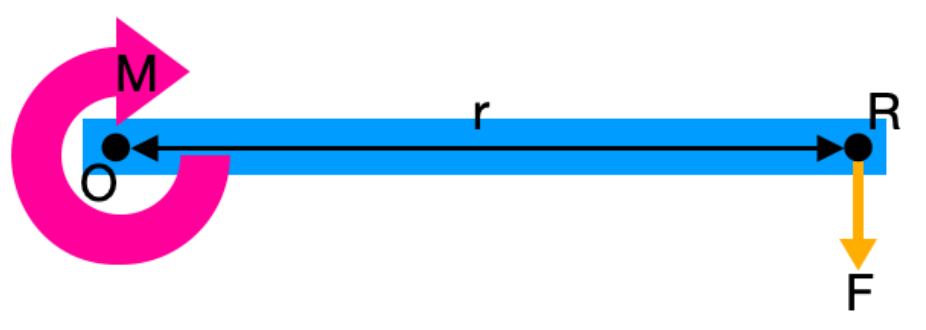
\includegraphics[width=\textwidth]{bonus_tests/drehmoment.png}


Das auf den Körper wirkende Drehmoment $\vec{M}$ ist das Kreuzprodukt $\vec{M} = \vec{r} \times \vec{F}$.

Im folgenden sei $\vec{r} = \begin{pmatrix}
        4 \\ 2 \\ -1
    \end{pmatrix}$ und $\vec{F} = \begin{pmatrix}
        2 \\ -3 \\ -6
    \end{pmatrix}$.

\subsection{a}
Berechnen Sie das auf den Körper wirkende Drehmoment $\vec{M}$.

\begin{align*}
    \vec{M} = \vec{r} \times \vec{F} \\
    = \begin{pmatrix}
        4 \\ 2 \\ -1 
    \end{pmatrix} \times \begin{pmatrix}
        2 \\ -3 \\ -6
    \end{pmatrix} \\
    = \begin{pmatrix}
        2 \cdot -6 - -1 \cdot -3 \\
        -1 \cdot 2 - 4 \cdot -6 \\
        4 \cdot -3 - 2 \cdot 2
    \end{pmatrix} \\
    \begin{pmatrix}
        -12 - 3 \\
        -2 - -24 \\
        -12 -4
    \end{pmatrix} \\
    \begin{pmatrix}
        -15 \\
        22 \\
        -16
    \end{pmatrix}
\end{align*}

\subsection{b}

Berechnen Sie den Betrag des Drehmoments und geben Sie das ergebnsi exakt an. 

\begin{align*}
    \left|\vec{M}\right| \\
    = \left|\begin{pmatrix}
        -15 \\ 22 \\ -16
    \end{pmatrix}\right| \\
    = \sqrt{-15^2 + 22^2 -16^2} \\
    = \sqrt{225 + 484 + 256} \\
    = \sqrt{965}
\end{align*}

	\part{Übungsaufgaben Lineare Algebra}
	\chapter{Übungsblatt 5}

\section{Aufgabe 1}
Bestimmen Sie die Ergebnisse der folgenden Rechenoperationen.

\subsection{a}
\begin{align*}
    3\begin{pmatrix} 1 \\ 1 \end{pmatrix} + 5 \begin{pmatrix} 4 \\ 1 \end{pmatrix}
     & = \begin{pmatrix} 3 \cdot 1 \\ 3 \cdot 1 \end{pmatrix} + \begin{pmatrix} 5 \cdot 4 \\ 5 \cdot 1 \end{pmatrix} \\
     & = \begin{pmatrix} 3 \\ 3 \end{pmatrix} + \begin{pmatrix} 20 \\ 5 \end{pmatrix}                                \\
     & = \begin{pmatrix} 3+20 \\ 3+5 \end{pmatrix}                                                                   \\
     & = \begin{pmatrix} 23 \\ 8 \end{pmatrix}
\end{align*}

\subsection{b}
\begin{align*}
    10\begin{pmatrix} 5 \\ 4 \\ 3 \end{pmatrix} + 4 \begin{pmatrix} 1 \\ 1 \\ 0 \end{pmatrix} + \begin{pmatrix} 3 \\ 2 \\ 1 \end{pmatrix}
     & = \begin{pmatrix} 10 \cdot 5 \\ 10 \cdot 4 \\ 10 \cdot 3 \end{pmatrix} + \begin{pmatrix} 4 \cdot 1 \\ 4 \cdot 1 \\ 4 \cdot 0 \end{pmatrix} + \begin{pmatrix} 3 \\ 2 \\ 1 \end{pmatrix} \\
     & = \begin{pmatrix} 50 \\ 40 \\ 30 \end{pmatrix} + \begin{pmatrix} 4 \\ 4 \\ 0 \end{pmatrix} + \begin{pmatrix} 3 \\ 2 \\ 1 \end{pmatrix}                                                 \\
     & = \begin{pmatrix} 50 + 4 + 3 \\ 40 + 4 + 2 \\ 30 + 0 + 1 \end{pmatrix}                                                                                                                 \\
     & = \begin{pmatrix} 57 \\ 46 \\ 31 \end{pmatrix}
\end{align*}

\hrulefill{}

\section{Aufgabe 2}

Sind die folgenden Mengen von Vektoren linear unabhängig? Können sie durch
Entfernen eines Vektors linear unabhängig gemacht werden?

Um auf lineare Unabhängigkeit zu prüfen, gibt es mehrere Möglichkeiten. Hier
zwei gängige Ansätze:

1.  Prüfung über die Determinante:
Man bildet aus den Vektoren eine quadratische Matrix $A$. Die Vektoren sind linear unabhängig, wenn die Determinante dieser Matrix
ungleich null ist ($\det(A) \neq 0$). Ist die Determinante gleich null ($\det(A) = 0$), sind die Vektoren linear abhängig.
(Diese Methode ist direkt nur anwendbar, wenn die Anzahl der Vektoren der Dimension des Raumes entspricht, z.B. 2 Vektoren im $\mathbb{R}^2$ oder 3 Vektoren im $\mathbb{R}^3$).

2.  Prüfung über die Definition der linearen Unabhängigkeit:
Eine Menge von Vektoren $\{v_1, v_2, \dots, v_n\}$ ist linear unabhängig, wenn die einzige Lösung der Vektorgleichung
\[ x_1v_1 + x_2v_2 + \cdots + x_n v_n = \mathbf{0} \]
die sogenannte triviale Lösung ist, bei der alle Skalare $x_1, x_2, \dots, x_n$
gleich null sind ($x_1 = x_2 = \cdots = x_n = 0$). Wenn es mindestens eine
nicht-triviale Lösung gibt (d.\ h.\ mindestens ein $x_i \neq 0$), dann sind die
Vektoren linear abhängig.

\subsection{a}
\[ \left\{ \begin{pmatrix} 1 \\ 1 \end{pmatrix}, \begin{pmatrix} 1 \\ 0 \end{pmatrix} \right\} \]

\subsubsection*{Prüfung für a über Determinante}
1.  Matrix aus den Vektoren erstellen:
\[ A = \begin{pmatrix} 1 & 1 \\ 1 & 0 \end{pmatrix} \]

2. Determinante der Matrix A berechnen
\begin{align*}
    \det(A) = A_{1,1} \cdot A_{2,2} - A_{2,1} \cdot A_{1,2} = 1 \cdot 0 - 1 \cdot 1 = 0 - 1 = -1
\end{align*}
Da die Determinante ungleich null ist, ist die Linearkombination linear unabhängig.

\subsubsection{Prüfung für a über Linearkombination}

\begin{align*}
    x_1 \cdot \begin{pmatrix}
                  1 \\1
              \end{pmatrix} + x_2 \cdot \begin{pmatrix}
                                            1 \\0
                                        \end{pmatrix} = \begin{pmatrix}
                                                            0 \\0
                                                        \end{pmatrix}            \\
    \begin{pmatrix}
        1 \cdot x_1 \\1 \cdot x_1
    \end{pmatrix} +\begin{pmatrix}
                       1 \cdot x_2 \\0 \cdot x_2
                   \end{pmatrix} = \begin{pmatrix}
                                       0 \\0
                                   \end{pmatrix}                                 \\
    \begin{pmatrix}
        1 \cdot x_1 + 1 \cdot x_2 \\1 \cdot x_1 + 0 \cdot x_2
    \end{pmatrix} = \begin{pmatrix}
                        0 \\0
                    \end{pmatrix}                          \\
    \begin{cases}
        \text{I:\@}  & 1 \cdot x_1 + 1  \cdot x_2 = 0 \\
        \text{II:\@} & 1 \cdot x_1 + 0 \cdot x_2 = 0
    \end{cases}                                 \\
    \begin{cases}
        \text{I:\@}  & x_1 + x_2 = 0              \\
        \text{II:\@} & x_1 \phantom{{} + x_2} = 0
    \end{cases} \\
    \text{in I einsetzen}                                                         \\
    0 + x_2 = 0                                                                   \\
    x_2 = 0
\end{align*}

Die einzige Lösung des linearen Gleichungssystem $x_1 = x_2 = 0$ ist, sind die
Vektoren linear unabhängig.

\subsection{b}
\[ \left\{ \begin{pmatrix} 1 \\ 1 \\ 1 \end{pmatrix},
    \begin{pmatrix} 1 \\ 0 \\ 1 \end{pmatrix}, \begin{pmatrix} 2 \\ 1 \\ 1 \end{pmatrix},
    \begin{pmatrix} 1 \\ 2 \\ 2 \end{pmatrix} \right\} \]

Es können nur drei Vektoren aus $\mathbb{R}^3$ linear unabhängig sein. Jede
Kombination aus mehr als drei Vektoren aus $\mathbb{R}^3$ ist linear abhängig.
Daher sind die vier Vektoren linear abhängig.

Um auf lineare Unabhängigkeit zu prüfen, wird ein beliebigen Vektor entfernt.\
hier wird der vierte Vektor entfernt.

Im schlimmsten Fall kann es passieren, dass vier Linearkombinationen auf
lineare Unabhängigkeit prüfen müssen, bis wir eine Linearkombination gefunden
wird, welche linear unabhängig ist.

\subsubsection{Prüfung für b über Determinante}
1.  Matrix aus den Vektoren erstellen:
\[ B = \begin{pmatrix} 1 & 1 & 2 \\ 1 & 0 & 1 \\ 1 & 1 & 1 \end{pmatrix} \]

2. Determinante der Matrix B berechnen
\begin{align*}
    \det(B) = B_{1,1} \cdot B_{2,2} \cdot B_{3,3} + B_{1,2} \cdot B_{2,3} \cdot B_{3,1} + B_{1,3} \cdot B_{2,1} \cdot B_{3,2} \\ - B_{3,1} \cdot B_{2,2} \cdot B_{1,3} - B_{3,2} \cdot B_{2,3} \cdot B_{1,1} - B_{3,3} \cdot B_{2,1} \cdot B_{1,2}\\
    = 1 \cdot 0 \cdot 1 + 1 \cdot 1 \cdot 1 + 2 \cdot 1 \cdot 1 - 1 \cdot 0 \cdot 2 - 1 \cdot 1 \cdot 1 - 1 \cdot 1 \cdot 1   \\
    = 0 + 1 + 2 - 0 - 1 - 1                                                                                                   \\
    = 1
\end{align*}
Da die Determinante ungleich null ist, kann die Vektormenge durch entfernen des vierten Vektors linear unabhängig gemacht werden.

\subsubsection{Prüfung für b über Linearkombination}
\begin{align*}
    x_1 \cdot \begin{pmatrix}
                  1 \\ 1 \\ 1
              \end{pmatrix} + x_2 \cdot \begin{pmatrix}
                                            1 \\ 0 \\ 1
                                        \end{pmatrix} + x_3 \cdot \begin{pmatrix}
                                                                      2 \\ 1 \\ 1
                                                                  \end{pmatrix} = \begin{pmatrix}
                                                                                      0 \\ 0 \\ 0
                                                                                  \end{pmatrix}                                                                                \\
    \begin{pmatrix}
        1 \cdot x_1 \\ 1 \cdot x_1 \\ 1 \cdot x_1
    \end{pmatrix} + \begin{pmatrix}
                        1 \cdot x_2 \\ 0 \cdot x_2 \\ 1 \cdot x_2
                    \end{pmatrix} + \begin{pmatrix}
                                        2 \cdot x_3 \\ 1 \cdot x_3 \\ 1 \cdot x_3
                                    \end{pmatrix} = \begin{pmatrix}
                                                        0 \\ 0 \\ 0
                                                    \end{pmatrix}                                                                                                    \\
    \begin{cases}
        \text{I:\@}   & 1 \cdot x_1 + 1 \cdot x_2 + 2 \cdot x_3 = 0 \\
        \text{II:\@}  & 1 \cdot x_1 + 0 \cdot x_2 + 1 \cdot x_3 = 0 \\
        \text{III:\@} & 1 \cdot x_1 + 1 \cdot x_2 + 1 \cdot x_3 = 0
    \end{cases}                                                                                                                 \\
    \begin{cases}
        \text{I:\@}   & x_1 + x_2 + 2x_3 = 0                                                                \\
        \text{II:\@}  & x_1 \phantom{{}+x_2} + \phantom{{}2}x_3 = 0 \quad | -x_3 \Leftrightarrow x_1 = -x_3 \\
        \text{III:\@} & x_1 + x_2 + \phantom{{}2}x_3 = 0
    \end{cases} \\
    x_1 \text{ in III einsetzen}                                                                                                                                                \\
    -x_3 + x_2 + x_3 = 0                                                                                                                                                        \\
    \Leftrightarrow x_2 = 0                                                                                                                                                     \\
    x_1 \text{ und } x_2 \text{ in I einsetzen}                                                                                                                                 \\
    -x_3 + 0 + 2x_3 = 0                                                                                                                                                         \\
    \Leftrightarrow -x_3 + 2x_3 = 0                                                                                                                                             \\
    \Leftrightarrow x_3 = 0                                                                                                                                                     \\
    x_3 \text{ in II einsetzen}                                                                                                                                                 \\
    x_1 + 0 = 0                                                                                                                                                                 \\
    \Leftrightarrow x_1 = 0
\end{align*}
Die einzige Lösung des linearen Gleichungssystem ist $x_1 = x_2 = x_3 = 0$, das heißt, dass die Vektormenge ohne den vierten Vektor linear unabhängig ist.

\hrulefill{}
\section{Aufgabe 3}
Bestimmen Sie die Dimension des Untervektorraums
\[ V := \text{span}\left\{ \begin{pmatrix} 1 \\ 1 \\ 1 \end{pmatrix}, \begin{pmatrix} 1 \\ 1 \\ 0 \end{pmatrix} \right\} \]

Die Dimension eines Untervektorraums ist die anzahl der Basisvektoren. Um
herauszufinden, ob die gegebenen Vektoren eines Basis des $\mathbb{R}^3$
bilden, muss auf lineare unabhängigkeit geprüft werden.

Hier bietet es sich nicht an, dies über die Determinante zu errechnen, da nur
quadratische Matzitzen eine Determinante besitzen.

\begin{align*}
    x_1 \cdot \begin{pmatrix}
                  1 \\ 1 \\1
              \end{pmatrix} + x_2 \cdot \begin{pmatrix}
                                            1 \\ 1 \\ 0
                                        \end{pmatrix} = \begin{pmatrix}
                                                            0 \\ 0 \\ 0
                                                        \end{pmatrix}             \\
    \begin{pmatrix}
        1 \cdot x_1 \\ 1 \cdot x_1 \\1 \cdot x_1
    \end{pmatrix} + \begin{pmatrix}
                        1 \cdot x_2 \\ 1 \cdot x_2 \\ 0 \cdot x_2
                    \end{pmatrix} = \begin{pmatrix}
                                        0 \\ 0 \\ 0
                                    \end{pmatrix}                       \\
    \begin{cases}
        \text{I:\@}   & 1 \cdot x_1 + 1 \cdot x_2 = 0 \\
        \text{II:\@}  & 1 \cdot x_1 + 1 \cdot x_2 = 0 \\
        \text{III:\@} & 1 \cdot x_1 + 0 \cdot x_2 = 0
    \end{cases}                                  \\
    \begin{cases}
        \text{I:\@}   & x_1 + x_2 = 0              \\
        \text{II:\@}  & x_1 + x_2 = 0              \\
        \text{III:\@} & x_1 \phantom{{} + x_2} = 0
    \end{cases} \\
    x_1 \text{ in I einsetzen}                                                     \\
    0 + x_2 = 0                                                                    \\
    \Leftrightarrow x_2 = 0
\end{align*}

Da $x_1 = x_2 = 0$ ist, ist die Vektormenge linear unabhängig. Diese zwei
linear unabhängigen Vektoren spannen den Untervektorraum V auf und bilden somit
eine Basis dieses Untervektorraums V. Da diese Basis aus zwei Vektoren besteht,
ist die Dimension des Untervektorraums V gleich 2.
	\chapter{Übungsblatt 6}

\section{Aufgabe 1}
Bestimmen Sie die Lösungsmengen der folgenden linearen Gleichungssysteme mit Hilfe des Gauß-Jordan-Algorithmus.

\subsection{a}
\begin{align*}
    \begin{cases}
        3x_1 + 2x_2 = 1 \\
        5x_1 + 4x_2 = 5
    \end{cases}
\end{align*}

\begin{longtable}{p{4cm}|p{3cm}}

    \hline
    \multicolumn{1}{c|}{\textbf{Linearkombination}} & \multicolumn{1}{c}{\textbf{Konstanten}} \\
    \hline
    \endfirsthead

    \hline
    \multicolumn{2}{c}{\tablename\ \thetable\ -- \textit{Fortführung von vorherier Seite}} \\
    \hline
    \multicolumn{1}{c|}{\textbf{Linearkombination}} & \multicolumn{1}{c}{\textbf{Konstanten}} \\
    \hline
    \endhead

    \hline
    \multicolumn{2}{r}{\textit{Fortsetzung siehe nächste Seite}} \\
    \endfoot

    \hline
    \endlastfoot

    $\displaystyle\begin{matrix}
      3 & 2 \\ 5 & 4
    \end{matrix}$&
    $\displaystyle\begin{matrix}
      1 \\ 5
    \end{matrix}$\\\hline

    \multicolumn{2}{p{\dimexpr4cm+3cm+2\tabcolsep\relax}}{Operation: 3II - 5I} \\\hline\pagebreak[0]

    $\displaystyle\begin{matrix}
      3 & 2 \\ 0 & 2
    \end{matrix}$&
    $\displaystyle\begin{matrix}
      1 \\ 10
    \end{matrix}$\\\hline

    \multicolumn{2}{p{\dimexpr4cm+3cm+2\tabcolsep\relax}}{Operation: I - II} \\\hline\pagebreak[0]

    $\displaystyle\begin{matrix}
      3 & 0 \\ 0 & 2
    \end{matrix}$&
    $\displaystyle\begin{matrix}
      -9 \\ 10
    \end{matrix}$\\\hline
    
    \multicolumn{2}{p{\dimexpr4cm+3cm+2\tabcolsep\relax}}{Operation: I : 3} \\\hline\pagebreak[0]
    \multicolumn{2}{p{\dimexpr4cm+3cm+2\tabcolsep\relax}}{Operation: II : 2} \\\hline\pagebreak[0]

    $\displaystyle\begin{matrix}
      1 & 0 \\ 0 & 1
    \end{matrix}$&
    $\displaystyle\begin{matrix}
      -3 \\ 5
    \end{matrix}$\\\hline

\end{longtable}


$x_1 = -3 \quad x_2 = 5$

\subsection{b)}
\begin{align*}    
  \begin{cases}
    \begin{aligned}
      x_1 &+ 2x_2 &- x_3 &= 10 \\
      15x_1 &+ x_2 &- 4x_3 &= 10 \\
      -x_1 &       &- 3x_3 &= 10
    \end{aligned}
  \end{cases}
\end{align*}

\begin{longtable}{p{4cm}|p{3cm}}

    \hline
    \multicolumn{1}{c|}{\textbf{Linearkombination}} & \multicolumn{1}{c}{\textbf{Konstanten}} \\
    \hline
    \endfirsthead

    \hline
    \multicolumn{2}{c}{\tablename\ \thetable\ -- \textit{Fortführung von vorherier Seite}} \\
    \hline
    \multicolumn{1}{c|}{\textbf{Linearkombination}} & \multicolumn{1}{c}{\textbf{Konstanten}} \\
    \hline
    \endhead

    \hline
    \multicolumn{2}{r}{\textit{Fortsetzung siehe nächste Seite}} \\
    \endfoot

    \hline
    \endlastfoot

    $\displaystyle\begin{matrix}
      1 & 2 & -1 \\ 15 & 1 & -4 \\ -1 & 0 & -3
    \end{matrix}$&
    $\displaystyle\begin{matrix}
      10 \\ 10 \\ 10
    \end{matrix}$\\\hline

    \multicolumn{2}{p{\dimexpr4cm+3cm+2\tabcolsep\relax}}{Operation: II + 15III} \\\hline\pagebreak[0]

    $\displaystyle\begin{matrix}
      1 & 2 & -1 \\ 0 & 1 & -49 \\ -1 & 0 & -3
    \end{matrix}$&
    $\displaystyle\begin{matrix}
      10 \\ 160 \\ 10
    \end{matrix}$\\\hline

    \multicolumn{2}{p{\dimexpr4cm+3cm+2\tabcolsep\relax}}{Operation: III + I} \\\hline\pagebreak[0]

    $\displaystyle\begin{matrix}
      1 & 2 & -1 \\ 0 & 1 & -49 \\ 0 & 2 & -4
    \end{matrix}$&
    $\displaystyle\begin{matrix}
      10 \\ 160 \\ 20
    \end{matrix}$\\\hline

    \multicolumn{2}{p{\dimexpr4cm+3cm+2\tabcolsep\relax}}{Operation: III - 2II} \\\hline\pagebreak[0]

    $\displaystyle\begin{matrix}
      1 & 2 & -1 \\ 0 & 1 & -49 \\ 0 & 0 & 94
    \end{matrix}$&
    $\displaystyle\begin{matrix}
      10 \\ 160 \\ -300
    \end{matrix}$\\\hline

    \multicolumn{2}{p{\dimexpr4cm+3cm+2\tabcolsep\relax}}{Operation: III : 94} \\\hline\pagebreak[0]

    $\displaystyle\begin{matrix}
      1 & 2 & -1 \\ 0 & 1 & -49 \\ 0 & 0 & 1
    \end{matrix}$&
    $\displaystyle\begin{matrix}
      10 \\ 160 \\ -\dfrac{150}{47}
    \end{matrix}$\\\hline

    \multicolumn{2}{p{\dimexpr4cm+3cm+2\tabcolsep\relax}}{Operation: I + III} \\\hline\pagebreak[0]

    $\displaystyle\begin{matrix}
      1 & 2 & 0 \\ 0 & 1 & -49 \\ 0 & 0 & 1
    \end{matrix}$&
    $\displaystyle\begin{matrix}
      \dfrac{320}{47} \\ 160 \\ -\dfrac{150}{47}
    \end{matrix}$\\\hline

    \multicolumn{2}{p{\dimexpr4cm+3cm+2\tabcolsep\relax}}{Operation: II + 49III} \\\hline\pagebreak[0]

    $\displaystyle\begin{matrix}
      1 & 2 & 0 \\ 0 & 1 & 0 \\ 0 & 0 & 1
    \end{matrix}$&
    $\displaystyle\begin{matrix}
      \dfrac{320}{47} \\ \dfrac{170}{47} \\ -\dfrac{150}{47}
    \end{matrix}$\\\hline

    \multicolumn{2}{p{\dimexpr4cm+3cm+2\tabcolsep\relax}}{Operation: I - 2II} \\\hline\pagebreak[0]

    $\displaystyle\begin{matrix}
      1 & 0 & 0 \\ 0 & 1 & 0 \\ 0 & 0 & 1
    \end{matrix}$&
    $\displaystyle\begin{matrix}
      -\dfrac{20}{47} \\ \dfrac{170}{47} \\ -\dfrac{150}{47}
    \end{matrix}$\\\hline

\end{longtable}

$x_1 = -\frac{20}{47}\quad x_2 = \frac{170}{47}\quad x_3 = -\frac{150}{47}$

\subsection{c)}
\begin{align*}    
  \begin{cases}
    \begin{aligned}
      x_1 - x_2 - x_3 = 1 \\
      x_1 + x_2 - x_3 = 2
    \end{aligned}
  \end{cases}
\end{align*}

\begin{longtable}{p{4cm}|p{3cm}}

    \hline
    \multicolumn{1}{c|}{\textbf{Linearkombination}} & \multicolumn{1}{c}{\textbf{Konstanten}} \\
    \hline
    \endfirsthead

    \hline
    \multicolumn{2}{c}{\tablename\ \thetable\ -- \textit{Fortführung von vorherier Seite}} \\
    \hline
    \multicolumn{1}{c|}{\textbf{Linearkombination}} & \multicolumn{1}{c}{\textbf{Konstanten}} \\
    \hline
    \endhead

    \hline
    \multicolumn{2}{r}{\textit{Fortsetzung siehe nächste Seite}} \\
    \endfoot

    \hline
    \endlastfoot

    $\displaystyle\begin{matrix}
      1 & -1 & -1 \\
      1 & 1 & -1
    \end{matrix}$&
    $\displaystyle\begin{matrix}
      1 \\ 2
    \end{matrix}$\\\hline

    \multicolumn{2}{p{\dimexpr4cm+3cm+2\tabcolsep\relax}}{Operation: II - I} \\\hline\pagebreak[0]

    $\displaystyle\begin{matrix}
      1 & -1 & -1 \\
     0 & 2 & 0
    \end{matrix}$&
    $\displaystyle\begin{matrix}
      1 \\ 1
    \end{matrix}$\\\hline

    \multicolumn{2}{p{\dimexpr4cm+3cm+2\tabcolsep\relax}}{Operation: 2I + II} \\\hline\pagebreak[0]

    $\displaystyle\begin{matrix}
      2 & 0 & -2 \\
     0 & 2 & 0
    \end{matrix}$&
    $\displaystyle\begin{matrix}
      3 \\ 1
    \end{matrix}$\\\hline

    \multicolumn{2}{p{\dimexpr4cm+3cm+2\tabcolsep\relax}}{Operation: I : 2} \\\hline\pagebreak[0]
    \multicolumn{2}{p{\dimexpr4cm+3cm+2\tabcolsep\relax}}{Operation: II : 2} \\\hline\pagebreak[0]

    $\displaystyle\begin{matrix}
      1 & 0 & -1 \\
     0 & 1 & 0
    \end{matrix}$&
    $\displaystyle\begin{matrix}
      \frac{3}{2} \\ \frac{1}{2}
    \end{matrix}$\\\hline

\end{longtable}

$x_2 = \frac{1}{2}$

$x_1 - x_3 = \frac{3}{2}$

$x_3 =: t \quad t \in \mathbb{R}$

$x_1 - t = \frac{3}{2} \quad | + t$

$\Leftrightarrow x_1 = \frac{3}{2} + t$

$\begin{pmatrix}
  x_1 \\ x_2 \\ x_3
\end{pmatrix} = \begin{pmatrix}
  \frac{3}{2} + t \\ \frac{1}{2} \\ t
\end{pmatrix}$ wobei $t \in \mathbb{R}$

\section{Aufgabe 2}

\subsection{a)}
Wenn fünf Ochsen und zwei Schafe acht Taels Gold kosten, sowie zwei Ochsen und acht Schafe auch acht Taels, was ist dann der Preis eines Tieres? (Chiu-Chang Suan-Chu, 300 n.Chr.)

$x_1 :=$ Ochsen \quad $x_2 :=$ Schafe

\begin{align*}
  \begin{cases}
    5x_1 + 2x_2 = 8 \\
    2x_1 + 8x_2 = 8
  \end{cases}
\end{align*}


\begin{longtable}{p{4cm}|p{3cm}}

    \hline
    \multicolumn{1}{c|}{\textbf{Linearkombination}} & \multicolumn{1}{c}{\textbf{Konstanten}} \\
    \hline
    \endfirsthead

    \hline
    \multicolumn{2}{c}{\tablename\ \thetable\ -- \textit{Fortführung von vorherier Seite}} \\
    \hline
    \multicolumn{1}{c|}{\textbf{Linearkombination}} & \multicolumn{1}{c}{\textbf{Konstanten}} \\
    \hline
    \endhead

    \hline
    \multicolumn{2}{r}{\textit{Fortsetzung siehe nächste Seite}} \\
    \endfoot

    \hline
    \endlastfoot

    $\displaystyle\begin{matrix}
      5 & 2 \\ 
      2 & 8
    \end{matrix}$&
    $\displaystyle\begin{matrix}
      8 \\ 8
    \end{matrix}$\\\hline

    \multicolumn{2}{p{\dimexpr4cm+3cm+2\tabcolsep\relax}}{Operation: 5II - 2I} \\\hline\pagebreak[0]

    $\displaystyle\begin{matrix}
      5 & 2 \\ 
      0 & 36
    \end{matrix}$&
    $\displaystyle\begin{matrix}
      8 \\ 24
    \end{matrix}$\\\hline

    \multicolumn{2}{p{\dimexpr4cm+3cm+2\tabcolsep\relax}}{Operation: 36I - 2II} \\\hline\pagebreak[0]

    $\displaystyle\begin{matrix}
      180 & 0 \\ 
      0 & 36
    \end{matrix}$&
    $\displaystyle\begin{matrix}
      240 \\ 24
    \end{matrix}$\\\hline

    \multicolumn{2}{p{\dimexpr4cm+3cm+2\tabcolsep\relax}}{Operation: I: 180} \\\hline\pagebreak[0]
    \multicolumn{2}{p{\dimexpr4cm+3cm+2\tabcolsep\relax}}{Operation: II: 36} \\\hline\pagebreak[0]

    $\displaystyle\begin{matrix}
      1 & 0 \\ 
      0 & 1
    \end{matrix}$&
    $\displaystyle\begin{matrix}
      \frac{4}{3} \\ \frac{3}{2}
    \end{matrix}$\\\hline

\end{longtable}

\subsection{b)}
Ein 9-Tupel $(x1, . . . , x9)$ nennt man \enquote{magisches Quadrat der Ordnung 3}, wenn gilt:
\begin{align*}    
    x1 + x2 + x3 = x4 + x5 + x6 = x7 + x8 + x9 = x1 + x4 + x7 \\ = x2 + x5 + x8 = x3 + x6 + x9 = x1 + x5 + x9 = x3 + x5 + x7
\end{align*}

Stellen Sie ein lineares Gleichungssystem auf, das zu diesen sieben Bedingungen äquivalent ist, und bestimmen Sie den Lösungsraum in $\mathbb{R}^9$. Wie kann man die Menge der rationalen Lösungen (also der $(x_1, \dots, x_9) \in \mathbb{Q}^9)$ beschrieben? Gibt es auch eine Lösung in $\mathbb{Z}^9$? Oder gar in $\mathbb{N}^9$? (siehe J. W. von Goethe 1: Faust. Der Tragödie erster Teil, Hexenküche).

(Diese Aufgaben sind entnommen aus: \textit{Peter Knaber, Wolf P. Barth:} Lineare Algebra. Aufgaben und Lösungen. \textit{Springer Verlag,} 2017. Seite 4.)

\begin{align*}
  \begin{cases}
    x_1 + x_2 + x_3 - x_4 - x_5 - x_6 = 0 \\
    x_4 + x_5 + x_6 - x_7 - x_8 - x_9 = 0 \\
    x_7 + x_8 + x_9 - x_1 - x_4 - x_7 = 0 \Rightarrow -x_1 -x_4 +x_8 +x_9 = 0\\
    x_1 + x_4 + x_7 - x_2 - x_5 - x_8 = 0 \Rightarrow x_1 - x_2 + x_4 - x_5 + x_7 - x_8\\
    x_2 + x_5 + x_8 - x_3 - x_6 - x_9 = 0 \Rightarrow x_2 - x_3 + x_5 - x_6 + x_8 - x_9\\
    x_3 + x_6 + x_9 - x_1 - x_5 - x_9 = 0 \Rightarrow - x_1 + x_3 - x_5 + x_6\\ 
    x_1 + x_5 + x_9 - x_3 - x_5 - x_7 = 0 \Rightarrow x_1 - x_3 - x_7 + x_9
  \end{cases} \\
\end{align*}

\begin{longtable}{p{10cm}}

    \hline
    \multicolumn{1}{c}{\textbf{Linearkombination}} \\
    \hline
    \endfirsthead

    \hline
    \multicolumn{1}{c}{\tablename\ \thetable\ -- \textit{Fortführung von vorherier Seite}} \\
    \hline
    \multicolumn{1}{c}{\textbf{Linearkombination}} \\
    \hline
    \endhead

    \hline
    \multicolumn{1}{r}{\textit{Fortsetzung siehe nächste Seite}} \\
    \endfoot

    \hline
    \endlastfoot

    $\displaystyle\begin{matrix}
    I & 1 & 1 & 1 & -1 & -1 & -1 & 0 & 0 & 0 \\
    II & 0 & 0 & 0 & 1 & 1 & 1 & -1 & -1 & -1 \\
    III & -1 & 0 & 0 & -1 & 0 & 0 & 0 & 1 & 1 \\
    IV & 1 & -1 & 0 & 1 & -1 & 0 & 1 & -1 & 0 \\
    V & 0 & 1 & -1 & 0 & 1 & -1 & 0 & 1 & -1 \\
    VI & -1 & 0 & 1 & 0 & -1 & 1 & 0 & 0 & 0 \\
    VII & 1 & 0 & -1 & 0 & 0 & 0 & -1 & 0 & 1
    \end{matrix}$\\\hline
    Ziel: erste Spalte bereinigen \\\hline\pagebreak[0]
    Operation: III + I \\\hline\pagebreak[0]
    $\displaystyle\begin{matrix}
    I & 1 & 1 & 1 & -1 & -1 & -1 & 0 & 0 & 0 \\
    II & 0 & 0 & 0 & 1 & 1 & 1 & -1 & -1 & -1 \\
    III & 0 & 1 & 1 & -2 & -1 & -1 & 0 & 1 & 1 \\
    IV & 1 & -1 & 0 & 1 & -1 & 0 & 1 & -1 & 0 \\
    V & 0 & 1 & -1 & 0 & 1 & -1 & 0 & 1 & -1 \\
    VI & -1 & 0 & 1 & 0 & -1 & 1 & 0 & 0 & 0 \\
    VII & 1 & 0 & -1 & 0 & 0 & 0 & -1 & 0 & 1
    \end{matrix}$\\\hline
    Operation: IV - I \\\hline\pagebreak[0]
    $\displaystyle\begin{matrix}
    I & 1 & 1 & 1 & -1 & -1 & -1 & 0 & 0 & 0 \\
    II & 0 & 0 & 0 & 1 & 1 & 1 & -1 & -1 & -1 \\
    III & 0 & 1 & 1 & -2 & -1 & -1 & 0 & 1 & 1 \\
    IV & 0 & -2 & -1 & 2 & 0 & 1 & 1 & -1 & 0 \\
    V & 0 & 1 & -1 & 0 & 1 & -1 & 0 & 1 & -1 \\
    VI & -1 & 0 & 1 & 0 & -1 & 1 & 0 & 0 & 0 \\
    VII & 1 & 0 & -1 & 0 & 0 & 0 & -1 & 0 & 1
    \end{matrix}$\\\hline
    Operation: VI + I \\\hline\pagebreak[0]
    $\displaystyle\begin{matrix}
    I & 1 & 1 & 1 & -1 & -1 & -1 & 0 & 0 & 0 \\
    II & 0 & 0 & 0 & 1 & 1 & 1 & -1 & -1 & -1 \\
    III & 0 & 1 & 1 & -2 & -1 & -1 & 0 & 1 & 1 \\
    IV & 0 & -2 & -1 & 2 & 0 & 1 & 1 & -1 & 0 \\
    V & 0 & 1 & -1 & 0 & 1 & -1 & 0 & 1 & -1 \\
    VI & 0 & 1 & 2 & -1 & -2 & 0 & 0 & 0 & 0 \\
    VII & 1 & 0 & -1 & 0 & 0 & 0 & -1 & 0 & 1
    \end{matrix}$\\\hline
    Operation: VII - I \\\hline\pagebreak[0]
    $\displaystyle\begin{matrix}
    I & 1 & 1 & 1 & -1 & -1 & -1 & 0 & 0 & 0 \\
    II & 0 & 0 & 0 & 1 & 1 & 1 & -1 & -1 & -1 \\
    III & 0 & 1 & 1 & -2 & -1 & -1 & 0 & 1 & 1 \\
    IV & 0 & -2 & -1 & 2 & 0 & 1 & 1 & -1 & 0 \\
    V & 0 & 1 & -1 & 0 & 1 & -1 & 0 & 1 & -1 \\
    VI & 0 & 1 & 2 & -1 & -2 & 0 & 0 & 0 & 0 \\
    VII & 0 & -1 & -2 & 1 & 1 & 1 & -1 & 0 & 1
    \end{matrix}$\\\hline
    Ziel: zweite Spalte bereinigen \\\hline\pagebreak[0]
    Operation: II und III tauschen \\\hline\pagebreak[0]
    $\displaystyle\begin{matrix}
    I & 1 & 1 & 1 & -1 & -1 & -1 & 0 & 0 & 0 \\
    II & 0 & 1 & 1 & -2 & -1 & -1 & 0 & 1 & 1 \\
    III & 0 & 0 & 0 & 1 & 1 & 1 & -1 & -1 & -1 \\
    IV & 0 & -2 & -1 & 2 & 0 & 1 & 1 & -1 & 0 \\
    V & 0 & 1 & -1 & 0 & 1 & -1 & 0 & 1 & -1 \\
    VI & 0 & 1 & 2 & -1 & -2 & 0 & 0 & 0 & 0 \\
    VII & 0 & -1 & -2 & 1 & 1 & 1 & -1 & 0 & 1
    \end{matrix}$\\\hline
    Operation: IV + 2V \\\hline\pagebreak[0]
    $\displaystyle\begin{matrix}
    I & 1 & 1 & 1 & -1 & -1 & -1 & 0 & 0 & 0 \\
    II & 0 & 1 & 1 & -2 & -1 & -1 & 0 & 1 & 1 \\
    III & 0 & 0 & 0 & 1 & 1 & 1 & -1 & -1 & -1 \\
    IV & 0 & 0 & -3 & 2 & 2 & -1 & 1 & 1 & -2 \\
    V & 0 & 1 & -1 & 0 & 1 & -1 & 0 & 1 & -1 \\
    VI & 0 & 1 & 2 & -1 & -2 & 0 & 0 & 0 & 0 \\
    VII & 0 & -1 & -2 & 1 & 1 & 1 & -1 & 0 & 1
    \end{matrix}$\\\hline
    Operation: V - VI \\\hline\pagebreak[0]
    $\displaystyle\begin{matrix}
    I & 1 & 1 & 1 & -1 & -1 & -1 & 0 & 0 & 0 \\
    II & 0 & 1 & 1 & -2 & -1 & -1 & 0 & 1 & 1 \\
    III & 0 & 0 & 0 & 1 & 1 & 1 & -1 & -1 & -1 \\
    IV & 0 & 0 & -3 & 2 & 2 & -1 & 1 & 1 & -2 \\
    V & 0 & 0 & -3 & 1 & 3 & -1 & 0 & 1 & -1 \\
    VI & 0 & 1 & 2 & -1 & -2 & 0 & 0 & 0 & 0 \\
    VII & 0 & -1 & -2 & 1 & 1 & 1 & -1 & 0 & 1
    \end{matrix}$\\\hline
    Operation: VI + VII \\\hline\pagebreak[0]
    $\displaystyle\begin{matrix}
    I & 1 & 1 & 1 & -1 & -1 & -1 & 0 & 0 & 0 \\
    II & 0 & 1 & 1 & -2 & -1 & -1 & 0 & 1 & 1 \\
    III & 0 & 0 & 0 & 1 & 1 & 1 & -1 & -1 & -1 \\
    IV & 0 & 0 & -3 & 2 & 2 & -1 & 1 & 1 & -2 \\
    V & 0 & 0 & -3 & 1 & 3 & -1 & 0 & 1 & -1 \\
    VI & 0 & 0 & 0 & 0 & -1 & 1 & -1 & 0 & 1 \\
    VII & 0 & -1 & -2 & 1 & 1 & 1 & -1 & 0 & 1
    \end{matrix}$\\\hline
    Operation: VII + II \\\hline\pagebreak[0]
    $\displaystyle\begin{matrix}
    I & 1 & 1 & 1 & -1 & -1 & -1 & 0 & 0 & 0 \\
    II & 0 & 1 & 1 & -2 & -1 & -1 & 0 & 1 & 1 \\
    III & 0 & 0 & 0 & 1 & 1 & 1 & -1 & -1 & -1 \\
    IV & 0 & 0 & -3 & 2 & 2 & -1 & 1 & 1 & -2 \\
    V & 0 & 0 & -3 & 1 & 3 & -1 & 0 & 1 & -1 \\
    VI & 0 & 0 & 0 & 0 & -1 & 1 & -1 & 0 & 1 \\
    VII & 0 & 0 & -1 & -1 & 0 & 0 & -1 & 1 & 2
    \end{matrix}$\\\hline
    Ziel: dritte Spalte bereinigen \\\hline\pagebreak[0]
    Operation: III und VII tauschen \\\hline\pagebreak[0]
    $\displaystyle\begin{matrix}
    I & 1 & 1 & 1 & -1 & -1 & -1 & 0 & 0 & 0 \\
    II & 0 & 1 & 1 & -2 & -1 & -1 & 0 & 1 & 1 \\
    III & 0 & 0 & -1 & -1 & 0 & 0 & -1 & 1 & 2 \\
    IV & 0 & 0 & -3 & 2 & 2 & -1 & 1 & 1 & -2 \\
    V & 0 & 0 & -3 & 1 & 3 & -1 & 0 & 1 & -1 \\
    VI & 0 & 0 & 0 & 0 & -1 & 1 & -1 & 0 & 1 \\
    VII & 0 & 0 & 0 & 1 & 1 & 1 & -1 & -1 & -1
    \end{matrix}$\\\hline
    Operation: IV - V \\\hline\pagebreak[0]
    $\displaystyle\begin{matrix}
    I & 1 & 1 & 1 & -1 & -1 & -1 & 0 & 0 & 0 \\
    II & 0 & 1 & 1 & -2 & -1 & -1 & 0 & 1 & 1 \\
    III & 0 & 0 & -1 & -1 & 0 & 0 & -1 & 1 & 2 \\
    IV & 0 & 0 & 0 & 1 & -1 & 0 & 1 & 0 & -1 \\
    V & 0 & 0 & -3 & 1 & 3 & -1 & 0 & 1 & -1 \\
    VI & 0 & 0 & 0 & 0 & -1 & 1 & -1 & 0 & 1 \\
    VII & 0 & 0 & 0 & 1 & 1 & 1 & -1 & -1 & -1
    \end{matrix}$\\\hline
    Operation: V - 3III \\\hline\pagebreak[0]
    $\displaystyle\begin{matrix}
    I & 1 & 1 & 1 & -1 & -1 & -1 & 0 & 0 & 0 \\
    II & 0 & 1 & 1 & -2 & -1 & -1 & 0 & 1 & 1 \\
    III & 0 & 0 & -1 & -1 & 0 & 0 & -1 & 1 & 2 \\
    IV & 0 & 0 & 0 & 1 & -1 & 0 & 1 & 0 & -1 \\
    V & 0 & 0 & 0 & 4 & 3 & -1 & 3 & -2 & -7 \\
    VI & 0 & 0 & 0 & 0 & -1 & 1 & -1 & 0 & 1 \\
    VII & 0 & 0 & 0 & 1 & 1 & 1 & -1 & -1 & -1
    \end{matrix}$\\\hline
    Operation: III $\cdot$ (-1) \\\hline\pagebreak[0]
    $\displaystyle\begin{matrix}
    I & 1 & 1 & 1 & -1 & -1 & -1 & 0 & 0 & 0 \\
    II & 0 & 1 & 1 & -2 & -1 & -1 & 0 & 1 & 1 \\
    III & 0 & 0 & 1 & 1 & 0 & 0 & 1 & -1 & -2 \\
    IV & 0 & 0 & 0 & 1 & -1 & 0 & 1 & 0 & -1 \\
    V & 0 & 0 & 0 & 4 & 3 & -1 & 3 & -2 & -7 \\
    VI & 0 & 0 & 0 & 0 & -1 & 1 & -1 & 0 & 1 \\
    VII & 0 & 0 & 0 & 1 & 1 & 1 & -1 & -1 & -1
    \end{matrix}$\\\hline
    Ziel: vierte Spalte bereinigen \\\hline\pagebreak[0]
    Operation: V - 4VII \\\hline\pagebreak[0]
    $\displaystyle\begin{matrix}
    I & 1 & 1 & 1 & -1 & -1 & -1 & 0 & 0 & 0 \\
    II & 0 & 1 & 1 & -2 & -1 & -1 & 0 & 1 & 1 \\
    III & 0 & 0 & 1 & 1 & 0 & 0 & 1 & -1 & -2 \\
    IV & 0 & 0 & 0 & 1 & -1 & 0 & 1 & 0 & -1 \\
    V & 0 & 0 & 0 & 0 & -1 & -5 & 7 & 2 & -3 \\
    VI & 0 & 0 & 0 & 0 & -1 & 1 & -1 & 0 & 1 \\
    VII & 0 & 0 & 0 & 1 & 1 & 1 & -1 & -1 & -1
    \end{matrix}$\\\hline
    Operation: VII - IV \\\hline\pagebreak[0]
    $\displaystyle\begin{matrix}
    I & 1 & 1 & 1 & -1 & -1 & -1 & 0 & 0 & 0 \\
    II & 0 & 1 & 1 & -2 & -1 & -1 & 0 & 1 & 1 \\
    III & 0 & 0 & 1 & 1 & 0 & 0 & 1 & -1 & -2 \\
    IV & 0 & 0 & 0 & 1 & -1 & 0 & 1 & 0 & -1 \\
    V & 0 & 0 & 0 & 0 & -1 & -5 & 7 & 2 & -3 \\
    VI & 0 & 0 & 0 & 0 & -1 & 1 & -1 & 0 & 1 \\
    VII & 0 & 0 & 0 & 0 & 2 & 1 & -2 & -1 & 0
    \end{matrix}$\\\hline
    Ziel: fünfte Spalte bereinigen \\\hline\pagebreak[0]
    Operation: 2VI + VII \\\hline\pagebreak[0]
    $\displaystyle\begin{matrix}
    I & 1 & 1 & 1 & -1 & -1 & -1 & 0 & 0 & 0 \\
    II & 0 & 1 & 1 & -2 & -1 & -1 & 0 & 1 & 1 \\
    III & 0 & 0 & 1 & 1 & 0 & 0 & 1 & -1 & -2 \\
    IV & 0 & 0 & 0 & 1 & -1 & 0 & 1 & 0 & -1 \\
    V & 0 & 0 & 0 & 0 & -1 & -5 & 7 & 2 & -3 \\
    VI & 0 & 0 & 0 & 0 & -1 & 1 & -1 & 0 & 1 \\
    VII & 0 & 0 & 0 & 0 & 0 & 3 & -4 & -1 & 2
    \end{matrix}$\\\hline
    Operation: VI - V \\\hline\pagebreak[0]
    $\displaystyle\begin{matrix}
    I & 1 & 1 & 1 & -1 & -1 & -1 & 0 & 0 & 0 \\
    II & 0 & 1 & 1 & -2 & -1 & -1 & 0 & 1 & 1 \\
    III & 0 & 0 & 1 & 1 & 0 & 0 & 1 & -1 & -2 \\
    IV & 0 & 0 & 0 & 1 & -1 & 0 & 1 & 0 & -1 \\
    V & 0 & 0 & 0 & 0 & -1 & -5 & 7 & 2 & -3 \\
    VI & 0 & 0 & 0 & 0 & 0 & 6 & -8 & -2 & 4 \\
    VII & 0 & 0 & 0 & 0 & 0 & 3 & -4 & -1 & 2
    \end{matrix}$\\\hline
    Operation: V $\cdot$ (-1) \\\hline\pagebreak[0]
    $\displaystyle\begin{matrix}
    I & 1 & 1 & 1 & -1 & -1 & -1 & 0 & 0 & 0 \\
    II & 0 & 1 & 1 & -2 & -1 & -1 & 0 & 1 & 1 \\
    III & 0 & 0 & 1 & 1 & 0 & 0 & 1 & -1 & -2 \\
    IV & 0 & 0 & 0 & 1 & -1 & 0 & 1 & 0 & -1 \\
    V & 0 & 0 & 0 & 0 & 1 & 5 & -7 & -2 & 3 \\
    VI & 0 & 0 & 0 & 0 & 0 & 6 & -8 & -2 & 4 \\
    VII & 0 & 0 & 0 & 0 & 0 & 3 & -4 & -1 & 2
    \end{matrix}$\\\hline
    Ziel: sechste Spalte bereinigen \\\hline\pagebreak[0]
    Operation: 2VII - VI \\\hline\pagebreak[0]
    $\displaystyle\begin{matrix}
    I & 1 & 1 & 1 & -1 & -1 & -1 & 0 & 0 & 0 \\
    II & 0 & 1 & 1 & -2 & -1 & -1 & 0 & 1 & 1 \\
    III & 0 & 0 & 1 & 1 & 0 & 0 & 1 & -1 & -2 \\
    IV & 0 & 0 & 0 & 1 & -1 & 0 & 1 & 0 & -1 \\
    V & 0 & 0 & 0 & 0 & 1 & 5 & -7 & -2 & 3 \\
    VI & 0 & 0 & 0 & 0 & 0 & 6 & -8 & -2 & 4 \\
    VII & 0 & 0 & 0 & 0 & 0 & 0 & 0 & 0 & 0
    \end{matrix}$\\\hline
    Operation: VI : 6 \\\hline\pagebreak[0]
    $\displaystyle\begin{matrix}
    I & 1 & 1 & 1 & -1 & -1 & -1 & 0 & 0 & 0 \\
    II & 0 & 1 & 1 & -2 & -1 & -1 & 0 & 1 & 1 \\
    III & 0 & 0 & 1 & 1 & 0 & 0 & 1 & -1 & -2 \\
    IV & 0 & 0 & 0 & 1 & -1 & 0 & 1 & 0 & -1 \\
    V & 0 & 0 & 0 & 0 & 1 & 5 & -7 & -2 & 3 \\
    VI & 0 & 0 & 0 & 0 & 0 & 1 & -\frac{4}{3} & -\frac{1}{3} & \frac{2}{3} \\
    VII & 0 & 0 & 0 & 0 & 0 & 0 & 0 & 0 & 0
    \end{matrix}$\\\hline
    Die siebte Zeile (VII) besteht ausschließlich aus nullen. Das bedeutet, 
    dass die ursprüngliche siebte Gleichung von den anderen linear abhängig 
    war und keine neuen Informationen liefert. Diese Zeile wird daher im 
    Folgenden nicht mehr berücksichtigt. \\\hline\pagebreak[0]
    $\displaystyle\begin{matrix}
    I & 1 & 1 & 1 & -1 & -1 & -1 & 0 & 0 & 0 \\
    II & 0 & 1 & 1 & -2 & -1 & -1 & 0 & 1 & 1 \\
    III & 0 & 0 & 1 & 1 & 0 & 0 & 1 & -1 & -2 \\
    IV & 0 & 0 & 0 & 1 & -1 & 0 & 1 & 0 & -1 \\
    V & 0 & 0 & 0 & 0 & 1 & 5 & -7 & -2 & 3 \\
    VI & 0 & 0 & 0 & 0 & 0 & 1 & -\frac{4}{3} & -\frac{1}{3} & \frac{2}{3}
    \end{matrix}$\\\hline
    Ziel: Einträge in Spalte sechs oberhalb des Pivots eleminieren \\\hline\pagebreak[0]
    Operation: V - 5VI \\\hline\pagebreak[0]
    $\displaystyle\begin{matrix}
    I & 1 & 1 & 1 & -1 & -1 & -1 & 0 & 0 & 0 \\
    II & 0 & 1 & 1 & -2 & -1 & -1 & 0 & 1 & 1 \\
    III & 0 & 0 & 1 & 1 & 0 & 0 & 1 & -1 & -2 \\
    IV & 0 & 0 & 0 & 1 & -1 & 0 & 1 & 0 & -1 \\
    V & 0 & 0 & 0 & 0 & 1 & 0 & -\frac{1}{3} & -\frac{1}{3} & -\frac{1}{3} \\
    VI & 0 & 0 & 0 & 0 & 0 & 1 & -\frac{4}{3} & -\frac{1}{3} & \frac{2}{3}
    \end{matrix}$\\\hline
    Operation: II + VI \\\hline\pagebreak[0]
    $\displaystyle\begin{matrix}
    I & 1 & 1 & 1 & -1 & -1 & -1 & 0 & 0 & 0 \\
    II & 0 & 1 & 1 & -2 & -1 & 0 & -\frac{4}{3} & \frac{2}{3} & \frac{5}{3} \\
    III & 0 & 0 & 1 & 1 & 0 & 0 & 1 & -1 & -2 \\
    IV & 0 & 0 & 0 & 1 & -1 & 0 & 1 & 0 & -1 \\
    V & 0 & 0 & 0 & 0 & 1 & 0 & -\frac{1}{3} & -\frac{1}{3} & -\frac{1}{3} \\
    VI & 0 & 0 & 0 & 0 & 0 & 1 & -\frac{4}{3} & -\frac{1}{3} & \frac{2}{3}
    \end{matrix}$\\\hline
    Operation: I + VI \\\hline\pagebreak[0]
    $\displaystyle\begin{matrix}
    I & 1 & 1 & 1 & -1 & -1 & 0 & -\frac{4}{3} & -\frac{1}{3} & \frac{2}{3} \\
    II & 0 & 1 & 1 & -2 & -1 & 0 & -\frac{4}{3} & \frac{2}{3} & \frac{5}{3} \\
    III & 0 & 0 & 1 & 1 & 0 & 0 & 1 & -1 & -2 \\
    IV & 0 & 0 & 0 & 1 & -1 & 0 & 1 & 0 & -1 \\
    V & 0 & 0 & 0 & 0 & 1 & 0 & -\frac{1}{3} & -\frac{1}{3} & -\frac{1}{3} \\
    VI & 0 & 0 & 0 & 0 & 0 & 1 & -\frac{4}{3} & -\frac{1}{3} & \frac{2}{3}
    \end{matrix}$\\\hline
    Ziel: Einträge in Spalte fünf oberhalb des Pivots eleminieren \\\hline\pagebreak[0]
    Operation: IV + V \\\hline\pagebreak[0]
    $\displaystyle\begin{matrix}
    I & 1 & 1 & 1 & -1 & -1 & 0 & -\frac{4}{3} & -\frac{1}{3} & \frac{2}{3} \\
    II & 0 & 1 & 1 & -2 & -1 & 0 & -\frac{4}{3} & \frac{2}{3} & \frac{5}{3} \\
    III & 0 & 0 & 1 & 1 & 0 & 0 & 1 & -1 & -2 \\
    IV & 0 & 0 & 0 & 1 & 0 & 0 & \frac{2}{3} & -\frac{1}{3} & -\frac{4}{3} \\
    V & 0 & 0 & 0 & 0 & 1 & 0 & -\frac{1}{3} & -\frac{1}{3} & -\frac{1}{3} \\
    VI & 0 & 0 & 0 & 0 & 0 & 1 & -\frac{4}{3} & -\frac{1}{3} & \frac{2}{3}
    \end{matrix}$\\\hline
    Operation: II + V \\\hline\pagebreak[0]
    $\displaystyle\begin{matrix}
    I & 1 & 1 & 1 & -1 & -1 & 0 & -\frac{4}{3} & -\frac{1}{3} & \frac{2}{3} \\
    II & 0 & 1 & 1 & -2 & 0 & 0 & -\frac{5}{3} & \frac{1}{3} & \frac{4}{3} \\
    III & 0 & 0 & 1 & 1 & 0 & 0 & 1 & -1 & -2 \\
    IV & 0 & 0 & 0 & 1 & 0 & 0 & \frac{2}{3} & -\frac{1}{3} & -\frac{4}{3} \\
    V & 0 & 0 & 0 & 0 & 1 & 0 & -\frac{1}{3} & -\frac{1}{3} & -\frac{1}{3} \\
    VI & 0 & 0 & 0 & 0 & 0 & 1 & -\frac{4}{3} & -\frac{1}{3} & \frac{2}{3}
    \end{matrix}$\\\hline
    Operation: I + V \\\hline\pagebreak[0]
    $\displaystyle\begin{matrix}
    I & 1 & 1 & 1 & -1 & 0 & 0 & -\frac{5}{3} & -\frac{2}{3} & \frac{1}{3} \\
    II & 0 & 1 & 1 & -2 & 0 & 0 & -\frac{5}{3} & \frac{1}{3} & \frac{4}{3} \\
    III & 0 & 0 & 1 & 1 & 0 & 0 & 1 & -1 & -2 \\
    IV & 0 & 0 & 0 & 1 & 0 & 0 & \frac{2}{3} & -\frac{1}{3} & -\frac{4}{3} \\
    V & 0 & 0 & 0 & 0 & 1 & 0 & -\frac{1}{3} & -\frac{1}{3} & -\frac{1}{3} \\
    VI & 0 & 0 & 0 & 0 & 0 & 1 & -\frac{4}{3} & -\frac{1}{3} & \frac{2}{3}
    \end{matrix}$\\\hline
    Ziel: Einträge in Spalte vier oberhalb des Pivots eleminieren \\\hline\pagebreak[0]
    Operation: III - IV \\\hline\pagebreak[0]
    $\displaystyle\begin{matrix}
    I & 1 & 1 & 1 & -1 & 0 & 0 & -\frac{5}{3} & -\frac{2}{3} & \frac{1}{3} \\
    II & 0 & 1 & 1 & -2 & 0 & 0 & -\frac{5}{3} & \frac{1}{3} & \frac{4}{3} \\
    III & 0 & 0 & 1 & 0 & 0 & 0 & \frac{1}{3} & -\frac{2}{3} & -\frac{2}{3} \\
    IV & 0 & 0 & 0 & 1 & 0 & 0 & \frac{2}{3} & -\frac{1}{3} & -\frac{4}{3} \\
    V & 0 & 0 & 0 & 0 & 1 & 0 & -\frac{1}{3} & -\frac{1}{3} & -\frac{1}{3} \\
    VI & 0 & 0 & 0 & 0 & 0 & 1 & -\frac{4}{3} & -\frac{1}{3} & \frac{2}{3}
    \end{matrix}$\\\hline
    Operation: II + 2IV \\\hline\pagebreak[0]
    $\displaystyle\begin{matrix}
    I & 1 & 1 & 1 & -1 & 0 & 0 & -\frac{5}{3} & -\frac{2}{3} & \frac{1}{3} \\
    II & 0 & 1 & 1 & 0 & 0 & 0 & -\frac{1}{3} & -\frac{1}{3} & -\frac{4}{3} \\
    III & 0 & 0 & 1 & 0 & 0 & 0 & \frac{1}{3} & -\frac{2}{3} & -\frac{2}{3} \\
    IV & 0 & 0 & 0 & 1 & 0 & 0 & \frac{2}{3} & -\frac{1}{3} & -\frac{4}{3} \\
    V & 0 & 0 & 0 & 0 & 1 & 0 & -\frac{1}{3} & -\frac{1}{3} & -\frac{1}{3} \\
    VI & 0 & 0 & 0 & 0 & 0 & 1 & -\frac{4}{3} & -\frac{1}{3} & \frac{2}{3}
    \end{matrix}$\\\hline
    Operation: I + IV \\\hline\pagebreak[0]
    $\displaystyle\begin{matrix}
    I & 1 & 1 & 1 & 0 & 0 & 0 & -1 & -1 & -1 \\
    II & 0 & 1 & 1 & 0 & 0 & 0 & -\frac{1}{3} & -\frac{1}{3} & -\frac{4}{3} \\
    III & 0 & 0 & 1 & 0 & 0 & 0 & \frac{1}{3} & -\frac{2}{3} & -\frac{2}{3} \\
    IV & 0 & 0 & 0 & 1 & 0 & 0 & \frac{2}{3} & -\frac{1}{3} & -\frac{4}{3} \\
    V & 0 & 0 & 0 & 0 & 1 & 0 & -\frac{1}{3} & -\frac{1}{3} & -\frac{1}{3} \\
    VI & 0 & 0 & 0 & 0 & 0 & 1 & -\frac{4}{3} & -\frac{1}{3} & \frac{2}{3}
    \end{matrix}$\\\hline
    Ziel: Einträge in Spalte drei oberhalb des Pivots eleminieren \\\hline\pagebreak[0]
    Operation: II - III \\\hline\pagebreak[0]
    $\displaystyle\begin{matrix}
    I & 1 & 1 & 1 & 0 & 0 & 0 & -1 & -1 & -1 \\
    II & 0 & 1 & 0 & 0 & 0 & 0 & -\frac{2}{3} & \frac{1}{3} & -\frac{2}{3} \\
    III & 0 & 0 & 1 & 0 & 0 & 0 & \frac{1}{3} & -\frac{2}{3} & -\frac{2}{3} \\
    IV & 0 & 0 & 0 & 1 & 0 & 0 & \frac{2}{3} & -\frac{1}{3} & -\frac{4}{3} \\
    V & 0 & 0 & 0 & 0 & 1 & 0 & -\frac{1}{3} & -\frac{1}{3} & -\frac{1}{3} \\
    VI & 0 & 0 & 0 & 0 & 0 & 1 & -\frac{4}{3} & -\frac{1}{3} & \frac{2}{3}
    \end{matrix}$\\\hline
    Operation: I - III \\\hline\pagebreak[0]
    $\displaystyle\begin{matrix}
    I & 1 & 1 & 0 & 0 & 0 & 0 & -\frac{4}{3} & -\frac{1}{3} & -\frac{1}{3} \\
    II & 0 & 1 & 0 & 0 & 0 & 0 & -\frac{2}{3} & \frac{1}{3} & -\frac{2}{3} \\
    III & 0 & 0 & 1 & 0 & 0 & 0 & \frac{1}{3} & -\frac{2}{3} & -\frac{2}{3} \\
    IV & 0 & 0 & 0 & 1 & 0 & 0 & \frac{2}{3} & -\frac{1}{3} & -\frac{4}{3} \\
    V & 0 & 0 & 0 & 0 & 1 & 0 & -\frac{1}{3} & -\frac{1}{3} & -\frac{1}{3} \\
    VI & 0 & 0 & 0 & 0 & 0 & 1 & -\frac{4}{3} & -\frac{1}{3} & \frac{2}{3}
    \end{matrix}$\\\hline
    Ziel: Einträge in Spalte zwei oberhalb des Pivots eleminieren \\\hline\pagebreak[0]
    Operation: I - II \\\hline\pagebreak[0]
    $\displaystyle\begin{matrix}
    I & 1 & 0 & 0 & 0 & 0 & 0 & -\frac{2}{3} & -\frac{2}{3} & \frac{1}{3} \\
    II & 0 & 1 & 0 & 0 & 0 & 0 & -\frac{2}{3} & \frac{1}{3} & -\frac{2}{3} \\
    III & 0 & 0 & 1 & 0 & 0 & 0 & \frac{1}{3} & -\frac{2}{3} & -\frac{2}{3} \\
    IV & 0 & 0 & 0 & 1 & 0 & 0 & \frac{2}{3} & -\frac{1}{3} & -\frac{4}{3} \\
    V & 0 & 0 & 0 & 0 & 1 & 0 & -\frac{1}{3} & -\frac{1}{3} & -\frac{1}{3} \\
    VI & 0 & 0 & 0 & 0 & 0 & 1 & -\frac{4}{3} & -\frac{1}{3} & \frac{2}{3}
    \end{matrix}$\\\hline

\end{longtable}

Hierraus lässt sich jetzt Schließen, dass 
\begin{align*}  
  x_1 -\frac{2}{3}x_7 - \frac{2}{3}x_8 + \frac{1}{3}x_9 = 0 \Leftrightarrow x_1 = \frac{2}{3}x_7 + \frac{2}{3}x_8 - \frac{1}{3}x_9, \\
  x_2 -\frac{2}{3}x_7 + \frac{1}{3}x_8 - \frac{2}{3}x_9 = 0 \Leftrightarrow x_2 = \frac{2}{3}x_7 - \frac{1}{3}x_8 + \frac{2}{3}x_9, \\
  x_3 + \frac{1}{3}x_7 - \frac{2}{3}x_8 - \frac{2}{3}x_9 = 0 \Leftrightarrow x_3 = - \frac{1}{3}x_7 + \frac{2}{3}x_8 + \frac{2}{3}x_9, \\
  x_4 + \frac{2}{3}x_7 - \frac{1}{3}x_8 - \frac{4}{3}x_9 = 0 \Leftrightarrow x_4 = - \frac{2}{3}x_7 + \frac{1}{3}x_8 + \frac{4}{3}x_9, \\
  x_5 -\frac{1}{3}x_7 - \frac{1}{3}x_8 - \frac{1}{3}x_9 = 0 \Leftrightarrow x_5 = \frac{1}{3}x_7 + \frac{1}{3}x_8 + \frac{1}{3}x_9, \\
  x_6 - \frac{4}{3}x_7 - \frac{1}{3}x_8 + \frac{2}{3}x_9 = 0 \Leftrightarrow x_6 = \frac{4}{3}x_7 + \frac{1}{3}x_8 - \frac{2}{3}x_9
\end{align*}

Also gilt 
\begin{align*}
  \begin{pmatrix}
    x_1 \\ x_2 \\ x_3 \\ x_4 \\ x_5 \\ x_6 \\ x_7 \\ x_8 \\ x_9
  \end{pmatrix} \displaybreak[2] \\ =
  \begin{pmatrix}
    \frac{2}{3}x_7 + \frac{2}{3}x_8 - \frac{1}{3}x_9 \\
    \frac{2}{3}x_7 - \frac{1}{3}x_8 + \frac{2}{3}x_9 \\ 
    - \frac{1}{3}x_7 + \frac{2}{3}x_8 + \frac{2}{3}x_9 \\
    - \frac{2}{3}x_7 + \frac{1}{3}x_8 + \frac{4}{3}x_9 \\
    \frac{1}{3}x_7 + \frac{1}{3}x_8 + \frac{1}{3}x_9 \\
    \frac{4}{3}x_7 + \frac{1}{3}x_8 - \frac{2}{3}x_9 \\
    x_7 \\
    x_8 \\
    x_9
  \end{pmatrix} \displaybreak[2] \\ = 
  \begin{pmatrix}
    \frac{2}{3}x_7\\
    \frac{2}{3}x_7 \\ 
    - \frac{1}{3}x_7 \\
    - \frac{2}{3}x_7 \\
    \frac{1}{3}x_7 \\
    \frac{4}{3}x_7 \\
    1x_7 \\
    0x_7 \\
    0x_7
  \end{pmatrix} + \begin{pmatrix}
    \frac{2}{3}x_8 \\
    -\frac{1}{3}x_8 \\ 
    \frac{2}{3}x_8 \\
    \frac{1}{3}x_8 \\
    \frac{1}{3}x_8 \\
    \frac{1}{3}x_8 \\
    0x_8 \\
    1x_8 \\
    0x_8
  \end{pmatrix} + \begin{pmatrix}
    - \frac{1}{3}x_9 \\
    \frac{2}{3}x_9 \\ 
    \frac{2}{3}x_9 \\
    \frac{4}{3}x_9 \\
    \frac{1}{3}x_9 \\
    - \frac{2}{3}x_9 \\
    0x_9 \\
    0x_9 \\
    1x_9
  \end{pmatrix} \displaybreak[2] \\ = x_7\begin{pmatrix}
    \frac{2}{3}\\
    \frac{2}{3} \\ 
    - \frac{1}{3} \\
    - \frac{2}{3} \\
    \frac{1}{3} \\
    \frac{4}{3} \\
    1 \\
    0 \\
    0
  \end{pmatrix} + x_8\begin{pmatrix}
    \frac{2}{3} \\
    -\frac{1}{3} \\ 
    \frac{2}{3} \\
    \frac{1}{3} \\
    \frac{1}{3} \\
    \frac{1}{3} \\
    0 \\
    1 \\
    0
  \end{pmatrix} + x_9\begin{pmatrix}
    - \frac{1}{3} \\
    \frac{2}{3} \\ 
    \frac{2}{3} \\
    \frac{4}{3} \\
    \frac{1}{3} \\
    - \frac{2}{3} \\
    0 \\
    0 \\
    1
  \end{pmatrix}
\end{align*}

wobei $x_7, x_8, x_9 \in \mathbb{R}$

Der Lösungsraum des Tupels in $\mathbb{R}^9$ ist also 

\[
L = \left\{
  x_7\begin{pmatrix}
    \frac{2}{3}\\
    \frac{2}{3} \\ 
    - \frac{1}{3} \\
    - \frac{2}{3} \\
    \frac{1}{3} \\
    \frac{4}{3} \\
    1 \\
    0 \\
    0
  \end{pmatrix} + x_8\begin{pmatrix}
    \frac{2}{3} \\
    -\frac{1}{3} \\ 
    \frac{2}{3} \\
    \frac{1}{3} \\
    \frac{1}{3} \\
    \frac{1}{3} \\
    0 \\
    1 \\
    0
  \end{pmatrix} + x_9\begin{pmatrix}
    - \frac{1}{3} \\
    \frac{2}{3} \\ 
    \frac{2}{3} \\
    \frac{4}{3} \\
    \frac{1}{3} \\
    - \frac{2}{3} \\
    0 \\
    0 \\
    1
  \end{pmatrix} \Bigg| x_7, x_8, x_9 \in \mathbb{R} 
  \right\}
\]

Die Menge der Rationalen Lösungen kann eingach beschrieben werden also

\[
L = \left\{
  x_7\begin{pmatrix}
    \frac{2}{3}\\
    \frac{2}{3} \\ 
    - \frac{1}{3} \\
    - \frac{2}{3} \\
    \frac{1}{3} \\
    \frac{4}{3} \\
    1 \\
    0 \\
    0
  \end{pmatrix} + x_8\begin{pmatrix}
    \frac{2}{3} \\
    -\frac{1}{3} \\ 
    \frac{2}{3} \\
    \frac{1}{3} \\
    \frac{1}{3} \\
    \frac{1}{3} \\
    0 \\
    1 \\
    0
  \end{pmatrix} + x_9\begin{pmatrix}
    - \frac{1}{3} \\
    \frac{2}{3} \\ 
    \frac{2}{3} \\
    \frac{4}{3} \\
    \frac{1}{3} \\
    - \frac{2}{3} \\
    0 \\
    0 \\
    1
  \end{pmatrix} \Bigg| x_7, x_8, x_9 \in \mathbb{Q} 
  \right\}
\]

Um eine Lösung in $\mathbb{Z}^9$ zu erhalten kann sichergestellt werden, dass alle Komponenten
ein vielfaches von drei sind. Hierfür kann beispielsweise die hinreichende, aber nicht notwendige Bedingung dass $x_7 = 3a, x_8 = 3b, x_9 = 3c$ mit $a, b, c \in \mathbb{Z}$ aufgestellt werden.

Man wähle beispielsweise $a = 1, b = 1, c = 1$, so erhält an das magische Quadrat 
\[
\begin{pmatrix}
  3 & 3 & 3 \\ 3 & 3 & 3 \\ 3 & 3 & 3
\end{pmatrix}
\]

Dieses ist auch eine Lösung für ein magisches Quadrat aus $\mathbb{N}^9$.

\section{Aufgabe 3}
Schreiben Sie den Gauß-Jordan-Algorithmus in Pseudocode auf.
\begin{lstlisting}
def gauss_jordan(matrix: list[list[float]], constants: list[list[float]] | None) -> list[list[float]]:
  n = len(matrix)
  m = len(matrix[0])
  i = 0

  while i < n and i < m:
    pivot_zeile = i

    for zeile in range(i + 1, n): # beste Zeile zum tauschen finden
      if abs(matrix[zeile][i]) > abs(matrix[pivot_zeile][i]):
        pivot_zeile = zeile

    if pivot_zeile != i: # Zeilen ggf. tauschen
      matrix[i], matrix[pivot_zeile] = matrix[pivot_zeile], matrix[i]  
      if constants:
        constants[i], constants[pivot_zeile] = constants[pivot_zeile], constants[i]

    if matrix[i][i] == 0:
      i += 1
      continue # Es gab keinen geeigneten Tauschkanidat. Eleminierung wird uebersprungen.
        
    pivot_wert = matrix[i][i]
    for k_norm in range(i, m):
      matrix[i][k_norm] = matrix[i][k_norm] / pivot_wert
    if constants and i < len(constants) and constants[i] is not None:
      for c_col in range(len(constants[i])):
        constants[i][c_col] = constants[i][c_col]  / pivot_wert

    for j in range(0, i): # Nullen oberhalb
        factor = matrix[j][i] / matrix[i][i]
        for k in range(i, m):
            matrix[j][k] = matrix[j][k] - matrix[i][k] * factor
        if constants and len(constants[0]) > 0:
            num_const_cols = len(constants[0])
            for c_col in range(num_const_cols):
                constants[j][c_col] = constants[j][c_col] - constants[i][c_col] * factor

    for j in range(i + 1, n): # Nullen unterhalb
        factor = matrix[j][i] / matrix[i][i]
        for k in range(i, m):
            matrix[j][k] = matrix[j][k] - matrix[i][k] * factor
        if constants and len(constants[0]) > 0:
            num_const_cols = len(constants[0])
            for c_col in range(num_const_cols):
                constants[j][c_col] = constants[j][c_col] - constants[i][c_col] * factor
    
    i += 1

  return matrix, constants
  
\end{lstlisting} 
	\allowdisplaybreaks 

\chapter{Übungsblatt 7}

\section{Aufgabe 1}

\subsection{a}
\begin{align*}
    A = \begin{pmatrix}
        1 & 2 & 3 \\ 1 & 5 & 0 \\ -1 & -1 & 7
    \end{pmatrix} \cdot \begin{pmatrix}
        4 & 2 & 1 \\ 1 & 6 & 1 \\ 0 & 1 & 7
    \end{pmatrix} \\
    = \begin{pmatrix}
        1 \cdot 4 + 2 \cdot 1 + 3 \cdot 0 & 1 \cdot 2 + 2 \cdot 6 + 3 \cdot 1 & 1 \cdot 1 + 2 \cdot 1 + 3 \cdot 7 \\
        1 \cdot 4 + 5 \cdot 1 + 0 \cdot 0 & 1 \cdot 2 + 5 \cdot 6 + 0 \cdot 1 & 1 \cdot 1 + 5 \cdot 1 + 0 \cdot 7 \\
        -1 \cdot 4 -1 \cdot 1 + 7 \cdot 4 & -1 \cdot 2 - 1 \cdot 6 + 7 \cdot 1 & -1 \cdot 1 - 1 \cdot 1 + 7 \cdot 7
    \end{pmatrix} \\
    \begin{pmatrix}
        6 & 17 & 24 \\ 9 & 32 & 6 \\ -5 & -1 & 47
    \end{pmatrix}
\end{align*}

\subsection{b}
\begin{align*}
    w = \begin{pmatrix}
        0 & 4 & 3 \\ 5 & 5 & 9 \\ 1 & 0 & 7
    \end{pmatrix} \cdot \begin{pmatrix}
        1 \\ 0 \\ 5
    \end{pmatrix} \\
    = \begin{pmatrix}
        0 \cdot 1 + 4 \cdot 0 + 3 \cdot 5 \\ 5 \cdot 1 + 5 \cdot 0 + 9 \cdot 5 \\ 1 \cdot 1 + 0 \cdot 0 + 7 \cdot 5
    \end{pmatrix} \\
    = \begin{pmatrix}
        15 \\ 50 \\ 36
    \end{pmatrix}
\end{align*}


\subsection{c}
\begin{align*}
    A \cdot w \\
    = \begin{pmatrix}
        6 \cdot 15 + 17 \cdot 50 + 24 \cdot 36 \\ 
        9 \cdot 15 + 32 \cdot 50 + 6 \cdot 36 \\ 
        -5 \cdot 15 - 1 \cdot 50 + 47 \cdot 36
    \end{pmatrix} \\
    = \begin{pmatrix}
        1804 \\ 1951 \\ 1567
    \end{pmatrix}
\end{align*}

\section{Aufgabe 2}

Gegeben seien die Vektoren 
\[
u_1 = \begin{pmatrix}
    1 \\ 2 \\ 0
\end{pmatrix}, u_2 = \begin{pmatrix}
    1 \\ -1 \\ 0
\end{pmatrix}, u_3 = \begin{pmatrix}
    0 \\ 0 \\ 1
\end{pmatrix}, u_4 = \begin{pmatrix}
    4 \\ 2 \\ 2
\end{pmatrix}, w = \begin{pmatrix}
    2 \\ 3 \\ 5
\end{pmatrix}
\]
sowie die lineare Abbildung $\varphi: \mathbb{R}^3 \rightarrow \mathbb{R}^3$ mit:
\[
\varphi(u_1) = \begin{pmatrix}
    0 \\ 1 \\ 0
\end{pmatrix},
\varphi(u_2) = \begin{pmatrix}
    1 \\ 2 \\ 3
\end{pmatrix},
\varphi(u_3) = \begin{pmatrix}
    2 \\ -1 \\ 7
\end{pmatrix}
\]

\subsection{a}
Zeigen Sie, dass die Vektoren $\{u_1, u_2, u_3\}$ eine Basis des $\mathbb{R}^3$ bilden.

Prüfen auf lineare Unabhängigkeit

\begin{align*}
    x_1u_1 + x_2u_2 + x_3u_3 = 0 \\
    \Leftrightarrow x_1\begin{pmatrix}
        1 \\ 2 \\ 0
    \end{pmatrix} + x_2\begin{pmatrix}
        1 \\ -1 \\ 0
    \end{pmatrix} + x_3\begin{pmatrix}
        0  \\ 0 \\ 1
    \end{pmatrix} = \begin{pmatrix}
        0 \\ 0 \\ 0
    \end{pmatrix} \\
    \Leftrightarrow \begin{pmatrix}
        x_1 \\ 2x_1 \\ 0
    \end{pmatrix} + \begin{pmatrix}
        x_2 \\ -x_2 \\ 0
    \end{pmatrix} + \begin{pmatrix}
        0  \\ 0 \\ x_3
    \end{pmatrix} = \begin{pmatrix}
        0 \\ 0 \\ 0
    \end{pmatrix} \\
    \begin{cases}
        \text{I:\@} & x_1 + x_2 = 0 \\
        \text{II:\@} & 2x_1 - x_2 = 0 \\
        \text{III:\@} & x_3 = 0 \\
    \end{cases} \\
    \text{I = II} \\
    x_1 + x_2 = 2x_1 - x_2 \quad | -x_1 \quad | +x_2 \\
    \Leftrightarrow  2x_2 = x_1 \\
    \Leftrightarrow x_1 = 2x_2 \\
    \text{in I einsetzen} \\
    2x_2 + x_2 = 0 \\
    \Leftrightarrow 3x_2 = 0 \quad | : 3 \\
    \Leftrightarrow x_2 = 0 \\
    x_1 = 2 \cdot 0 \\
    \Leftrightarrow x_1 = 0
\end{align*}

Die einzige Lösung des linearen Gleichungssystems ist $x_1 = x_2 = x_3 = 0$. Das bedeutet, 
dass die Vektoren $\left\{u_1, u_2, u_3\right\}$ linear unabhängig sind. Dementsprechend bilden sie 
eine Basis des $\mathbb{R}^3$

\subsection{b}
Berechnen Sie $\varphi(u_4)$

\begin{align*}
    \begin{pmatrix}
        1 & 1 & 0 \\ 2 & -1 & 0 \\ 0 & 0 & 1
    \end{pmatrix} \cdot \begin{pmatrix}
        x_1 \\ x_2 \\ x_3
    \end{pmatrix} = \begin{pmatrix}
        4 \\ 2 \\ 2
    \end{pmatrix} \\
    \begin{cases}
        \text{I:\@} & x_1 + x_2 = 4\\
        \text{II:\@} & 2x_1 - x_2 = 2\\
        \text{III:\@} & x_3 = 2
    \end{cases} \\
    \text{I + II}
    \begin{cases}
        \text{I:\@} & 3x_1 = 6 \quad | :3 \Leftrightarrow x_1 = 2 \\
        \text{II:\@} & 2x_1 - x_2 = 2\\
        \text{III:\@} & x_3 = 2
    \end{cases} \\
    \text{in II einsetzen} \\
    2 \cdot 2 - x_2 = 2 \\
    \Leftrightarrow 4 - x_2 = 2 \quad | -4 \quad | \cdot(-1) \\
    \Leftrightarrow x_2 = 2
\end{align*}

$u_4$ ist linear abhängig zu den Vektoren $\left\{u_1, u_2, u_3\right\}$ mit den Faktor 2.

\begin{align*}
    u_1, u_2, u_3 = u_4 \\
    \varphi(u_1), \varphi(u_2), \varphi(u_3) = \varphi(u_4) \\
    \begin{pmatrix}
        0 & 1 & 2 \\ 1 & 2 & -1 \\ 0 & 3 & 7
    \end{pmatrix} \cdot \begin{pmatrix}
        2 \\ 2 \\ 2
    \end{pmatrix} = \varphi(u_4) \\
    2 \cdot \begin{pmatrix}
        0 \\ 1 \\ 0
    \end{pmatrix} + 2 \cdot \begin{pmatrix}
        1 \\ 2 \\ 3
    \end{pmatrix} + 2 \cdot \begin{pmatrix}
        2 \\ -1 \\ 7
    \end{pmatrix} = \varphi(u_4) \\
    = \begin{pmatrix}
        0 \\ 2 \\ 0
    \end{pmatrix} + \begin{pmatrix}
        2 \\ 4 \\ 6
    \end{pmatrix} + \begin{pmatrix}
        4 \\ -2 \\ 14
    \end{pmatrix} = \varphi(u_4) \\
    = \begin{pmatrix}
        6 \\ 4 \\ 20
    \end{pmatrix} = \varphi(u_4)
\end{align*}

\subsection{c}
Geben Sie einen Vektor $u_5$ an, mit $\varphi(u_5) = w$.

\begin{align*}
    \varphi(u_5) = x_1 \cdot \varphi(u_1) + x_2 \cdot \varphi(u_2) + x_3 \cdot \varphi(u_3) \\
    \varphi(u_5) = x_1 \cdot \begin{pmatrix}
        0 \\ 1 \\ 0
    \end{pmatrix} + x_2 \cdot \begin{pmatrix}
        1 \\ 2 \\ 3
    \end{pmatrix} + x_3 \cdot \begin{pmatrix}
        2 \\ -1 \\ 7
    \end{pmatrix} = \begin{pmatrix}
        2 \\ 3 \\ 5
    \end{pmatrix} \\
    \begin{cases}
        \text{I:\@} & x_2 + 2x_3 = 2\\
        \text{II:\@} & x_1 + 2x_2 - x_3 = 3\\
        \text{III:\@} & 3x_2 + 7x_3 = 5 
    \end{cases}
\end{align*}

\begin{longtable}{p{4cm}|p{3cm}}

    \hline
    \multicolumn{1}{c|}{\textbf{Linearkombination}} & \multicolumn{1}{c}{\textbf{Konstanten}} \\
    \hline
    \endfirsthead

    \hline
    \multicolumn{2}{c}{\tablename\ \thetable\ -- \textit{Fortführung von vorherier Seite}} \\
    \hline
    \multicolumn{1}{c|}{\textbf{Linearkombination}} & \multicolumn{1}{c}{\textbf{Konstanten}} \\
    \hline
    \endhead

    \hline
    \multicolumn{2}{r}{\textit{Fortsetzung siehe nächste Seite}} \\
    \endfoot

    \hline
    \endlastfoot

    $\displaystyle\begin{matrix}
        0 & 1 & 2 \\
        1 & 2 & -1 \\
        0 & 3 & 7
    \end{matrix}$&
    $\displaystyle\begin{matrix}
        2 \\ 3 \\ 5
    \end{matrix}$\\\hline

    \multicolumn{2}{p{\dimexpr4cm+3cm+2\tabcolsep\relax}}{Operation: I und II tauschen} \\\hline\pagebreak[0]

    $\displaystyle\begin{matrix}
        1 & 2 & -1 \\
        0 & 1 & 2 \\
        0 & 3 & 7
    \end{matrix}$&
    $\displaystyle\begin{matrix}
        3 \\ 2 \\ 5
    \end{matrix}$\\\hline

    \multicolumn{2}{p{\dimexpr4cm+3cm+2\tabcolsep\relax}}{Operation: III - 3II} \\\hline\pagebreak[0]

    $\displaystyle\begin{matrix}
        1 & 2 & -1 \\
        0 & 1 & 2 \\
        0 & 0 & 1
    \end{matrix}$&
    $\displaystyle\begin{matrix}
        3 \\ 2 \\ -1
    \end{matrix}$\\\hline

    \multicolumn{2}{p{\dimexpr4cm+3cm+2\tabcolsep\relax}}{Operation: II - 2III} \\\hline\pagebreak[0]

    $\displaystyle\begin{matrix}
        1 & 2 & -1 \\
        0 & 1 & 0 \\
        0 & 0 & 1
    \end{matrix}$&
    $\displaystyle\begin{matrix}
        3 \\ 4 \\ -1
    \end{matrix}$\\\hline

    \multicolumn{2}{p{\dimexpr4cm+3cm+2\tabcolsep\relax}}{Operation: I + III} \\\hline\pagebreak[0]

    $\displaystyle\begin{matrix}
        1 & 2 & 0 \\
        0 & 1 & 0 \\
        0 & 0 & 1
    \end{matrix}$&
    $\displaystyle\begin{matrix}
        2 \\ 4 \\ -1
    \end{matrix}$\\\hline

    \multicolumn{2}{p{\dimexpr4cm+3cm+2\tabcolsep\relax}}{Operation: I - 2II} \\\hline\pagebreak[0]

    $\displaystyle\begin{matrix}
        1 & 0 & 0 \\
        0 & 1 & 0 \\
        0 & 0 & 1
    \end{matrix}$&
    $\displaystyle\begin{matrix}
        -6 \\ 4 \\ -1
    \end{matrix}$\\\hline
\end{longtable}

\begin{align*}
    x_1 = -6, \quad x_2 = 4, \quad x_3 = -1 \\
    u_5 = -6 \cdot \begin{pmatrix}
        1 \\ 2 \\ 0
    \end{pmatrix} + 4 \cdot \begin{pmatrix}
        1 \\ -1 \\ 0
    \end{pmatrix} - 1 \cdot \begin{pmatrix}
        0 \\ 0 \\ 1
    \end{pmatrix} \\
    = \begin{pmatrix}
        -6 \\ -12 \\ 0
    \end{pmatrix} + \begin{pmatrix}
        4 \\-4 \\ 0
    \end{pmatrix} + \begin{pmatrix}
        0 \\ 0 \\ -1
    \end{pmatrix} \\
    = \begin{pmatrix}
        -2 \\ -16 \\ -1
    \end{pmatrix} = u_5
\end{align*}

\subsection{d}
Geben Sie die lineare Abbildung $\varphi$ in der Form $\varphi(x) = Ax$ an.

\begin{align*}
    c_{1,1} \cdot \begin{pmatrix}
        1 \\ 2 \\ 0
    \end{pmatrix} + c_{2, 1} \cdot \begin{pmatrix}
        1 \\ -1 \\ 0
    \end{pmatrix} + c_{3, 1} \cdot \begin{pmatrix}
        0 \\ 0 \\ 1
    \end{pmatrix} = \begin{pmatrix}
        1 \\ 0 \\ 0
    \end{pmatrix} \\
    \begin{cases}
        \text{I:\@} & c_{1,1} + c_{2,1} = 1 \\
        \text{II:\@} & 2c_{1,1} - c_{2,1} = 0 \\
        \text{III:\@} & c_{3,1} = 0
    \end{cases} \\
    \text{I + II} \\ 
    \begin{cases}
        \text{I:\@} & 3c_{1,1}  = 1 \quad | : 3 \Leftrightarrow c_{1,1} = \frac{1}{3}\\
        \text{II:\@} & 2c_{1,1} - c_{2,1} = 0 \\
        \text{III:\@} & c_{3,1} = 0
    \end{cases} \\
    \text{in II einsetzen} \\
    \begin{cases}
        \text{I:\@} & c_{1,1} = \frac{1}{3}\\
        \text{II:\@} & 2 \cdot \frac{1}{3} - c_{2, 1} = 0 \quad | +c_{2, 1} \Leftrightarrow \frac{2}{3} = c_{2, 1}  \\
        \text{III:\@} & c_{3,1} = 0
    \end{cases} \\
\end{align*}

\begin{align*}
    c_{1,2} \cdot \begin{pmatrix}
        1 \\ 2 \\ 0
    \end{pmatrix} + c_{2, 2} \cdot \begin{pmatrix}
        1 \\ -1 \\ 0
    \end{pmatrix} + c_{3, 2} \cdot \begin{pmatrix}
        0 \\ 0 \\ 1
    \end{pmatrix} = \begin{pmatrix}
        0 \\ 1 \\ 0
    \end{pmatrix} \\
    \begin{cases}
        \text{I:\@} & c_{1,2} + c_{2,2} = 0 \\
        \text{II:\@} & 2c_{1,2} - c_{2,2} = 1 \\
        \text{III:\@} & c_{3,2} = 0
    \end{cases} \\
    \text{I + II} \\
    \begin{cases}
        \text{I:\@} & 3c_{1,2}  = 1 \quad | : 3 \Leftrightarrow c_{1,2} = \frac{1}{3}\\
        \text{II:\@} & 2c_{1,2} - c_{2,2} = 1 \\
        \text{III:\@} & c_{3,2} = 0
    \end{cases} \\
    \text{in II einsetzen} \\
    \begin{cases}
        \text{I:\@} & c_{1,2} = \frac{1}{3}\\
        \text{II:\@} & 2 \cdot \frac{1}{3} - c_{2, 2} = 1 \quad | + c_{2, 2}  \quad | -1 \Leftrightarrow -\frac{1}{3} = c_{2, 2}\\
        \text{III:\@} & c_{3,2} = 0
    \end{cases} \\
\end{align*}

\begin{align*}
    c_{1,3} \cdot \begin{pmatrix}
        1 \\ 2 \\ 0
    \end{pmatrix} + c_{2, 3} \cdot \begin{pmatrix}
        1 \\ -1 \\ 0
    \end{pmatrix} + c_{3, 3} \cdot \begin{pmatrix}
        0 \\ 0 \\ 1
    \end{pmatrix} = \begin{pmatrix}
        0 \\ 0 \\ 1
    \end{pmatrix} \\
    \begin{cases}
        \text{I:\@} & c_{1,3} + c_{2,3} = 0 \\
        \text{II:\@} & 2c_{1,3} - c_{2,3} = 0 \\
        \text{III:\@} & c_{3,3} = 1
    \end{cases} \\
    \text{I + II} \\
    \begin{cases}
        \text{I:\@} & 3c_{1,3}  = 0 \quad | : 3 \Leftrightarrow c_{1,3} = 0\\
        \text{II:\@} & 2c_{1,3} - c_{2,3} = 0 \\
        \text{III:\@} & c_{3,3} = 1
    \end{cases} \\
    \text{in II einsetzen} \\
    \begin{cases}
        \text{I:\@} & c_{1,3} = 0\\
        \text{II:\@} & 2 \cdot 0 - c_{2, 3} = 0 \quad | \cdot (-1) \Leftrightarrow c_{2, 3} = 0\\
        \text{III:\@} & c_{3,3} = 1
    \end{cases} \\
\end{align*}

\begin{align*}
    \varphi(e_1) = \frac{1}{3} \cdot \varphi(u_1) + \frac{2}{3} \varphi(u_2) \\
    \varphi(e_1) = \frac{1}{3} \cdot \begin{pmatrix}
        0 \\ 1 \\ 0
    \end{pmatrix} + \frac{2}{3} \cdot \begin{pmatrix}
        1 \\ 2 \\ 3
    \end{pmatrix} \\
    \varphi(e_1) = \begin{pmatrix}
        0 \\ \frac{1}{3} \\ 0
    \end{pmatrix} + \begin{pmatrix}
        \frac{2}{3} \\ \frac{4}{3} \\ 2
    \end{pmatrix} \\
    \varphi(e_1) = \begin{pmatrix}
        \frac{2}{3} \\ \frac{5}{3} \\ 2 
    \end{pmatrix}\\
    \varphi(e_2) = \frac{1}{3} \cdot \varphi(u_1) - \frac{1}{3} \cdot \varphi(u_2) \\
    \varphi(e_2) = \frac{1}{3} \cdot \begin{pmatrix}
        0 \\ 1 \\ 0
    \end{pmatrix} -\frac{1}{3} \cdot \begin{pmatrix}
        1 \\ 2 \\ 3
    \end{pmatrix} \\
    \varphi(e_2) = \begin{pmatrix}
        0 \\ \frac{1}{3} \\ 0
    \end{pmatrix} + \begin{pmatrix}
        -\frac{1}{3} \\ -\frac{2}{3} \\ -1
    \end{pmatrix} \\
    \varphi(e_2) = \begin{pmatrix}
        -\frac{1}{3} \\ -\frac{1}{3} \\ -1
    \end{pmatrix}\\
    \varphi(e_3) = \varphi(u_3) \\
    \varphi(e_3) = \begin{pmatrix}
        2 \\ -1 \\ 7
    \end{pmatrix} \\
    A = \begin{pmatrix}
        \frac{2}{3} & -\frac{1}{3} & 2 \\
        \frac{5}{3} & -\frac{2}{3} & -1 \\
        2 & -1 & 7
    \end{pmatrix}\\
    \varphi(x) = \begin{pmatrix}
        \frac{2}{3} & -\frac{1}{3} & 2 \\
        \frac{5}{3} & -\frac{2}{3} & -1 \\
        2 & -1 & 7
    \end{pmatrix} \cdot \begin{pmatrix}
        x_1 \\ x_2 \\ x_3
    \end{pmatrix}
\end{align*}

\section{Aufgabe 3}

\subsection{a}
Bestimmen Sie eine lineare Abbildung $T: \mathbb{R}^3 \rightarrow \mathbb{R}^3$, deren Kern nur den Nullvektor enthält. Bestimmen Sie weiterhin eine lineare Abbildung $S: \mathbb{R}^3 \rightarrow \mathbb{R}^3$, deren Kern der gesamte Raum $\mathbb{R}^3$ ist.

\[
T = \begin{pmatrix}
    1 & 0 & 0 \\
    0 & 1 & 0 \\
    0 & 0 & 1
\end{pmatrix}
\]

\[
S = \begin{pmatrix}
    0 & 0 & 0 \\
    0 & 0 & 0 \\ 
    0 & 0 & 0
\end{pmatrix}
\]

\subsection{b}
Bestimmen Sie Bild und Kern der Matrix
\[
A=\begin{pmatrix}
    2 & 2 & 3 \\ 1 & 1 & 0 \\ -1 & -1 & 1
\end{pmatrix}
\]

\subsection*{Bild}

\begin{align*}
    n = \dim(Bild(A)) + \dim(Kern(A)) \\
    3 = \dim(Bild(A)) + 1 \quad |-1 \\
    \Leftrightarrow  2 = \dim(Bild(A))
\end{align*}

\subsection*{Kern}
\begin{align*}
    \begin{pmatrix}
    2 & 2 & 3 \\ 1 & 1 & 0 \\ -1 & -1 & 1
\end{pmatrix} \cdot \begin{pmatrix}
    x_1 \\ x_2 \\ x_3
\end{pmatrix} = \begin{pmatrix}
    0 \\ 0 \\ 0
\end{pmatrix} \\\pagebreak[0]
\begin{cases}
    \text{I:\@} & 2x_1 + 2x_2 + 3x_3 = 0 \\
    \text{II:\@} & x_1 + x_2 = 0 \\
    \text{III:\@} & -x_1 - x_2 + x_3 = 0
\end{cases} \\\pagebreak[0]
\text{III + II} \\\pagebreak[0]
\begin{cases}
    \text{I:\@} & 2x_1 + 2x_2 + 3x_3 = 0 \\
    \text{II:\@} & x_1 + x_2 = 0 \\
    \text{III:\@} & x_3 = 0
\end{cases} \\
\text{in I einsetzen} \\\pagebreak[0]
\begin{cases}
    \text{I:\@} & 2x_1 + 2x_2 + 3 \cdot 0 = 0 \Leftrightarrow 2x_1 + 2x_2 = 0 \\
    \text{II:\@} & x_1 + x_2 = 0 \quad | -x_2 \Leftrightarrow x_1 = -x_2\\
    \text{III:\@} & x_3 = 0
\end{cases} \\\pagebreak[0]
\text{in I einsetzen} \\\pagebreak[0]
\begin{cases}
    \text{I:\@} & 2 \cdot -x_2 + 2x_2 = 0 \Leftrightarrow 0 = 0 \\
    \text{II:\@} & x_1 = -x_2\\
    \text{III:\@} & x_3 = 0
\end{cases} \\\pagebreak[0]
\begin{pmatrix}
    x_1 \\ x_2 \\ x_3
\end{pmatrix} = \begin{pmatrix}
    -x_2 \\ x_2 \\ 0
\end{pmatrix} \text{, wobei } x_2 \in \mathbb{R} \\
span\left\{\begin{pmatrix}
    -1 \\ 1 \\ 0
\end{pmatrix}\right\}
\end{align*}

\section{Aufgabe 4}

\subsection{a}
Es sei $T: \mathbb{R}^3 \rightarrow \mathbb{R}^3$ gegeben durch: $T \begin{pmatrix} x \\ y \\ z \end{pmatrix} = \begin{pmatrix}2x \\ 4x-y \\ 2x+3y\end{pmatrix}$. Zeigen Sie, dass $T$ invertierbar ist, und geben Sie eine Formel für $T^{-1}$ an.

\subsubsection*{Prüfen, ob Matrix invertierbar ist}
Dass eine Matrix invertierbar ist, muss sie linear unabhängig sein. $\rightarrow \det(T) \neq 0$.
\begin{align*}
    \det\left(\begin{pmatrix}
        2 & 0 & 0 \\
        4 & -1 & 0 \\
        2 & 3 & 0
    \end{pmatrix}\right) = 2 \cdot -1 \cdot 0 + 0 \cdot 0 \cdot 0 + 0 \cdot 4 \cdot 3 \\
    - 2 \cdot -1 \cdot 0 - 3 \cdot 0 \cdot 0 - 0 \cdot 4 \cdot 0 \\
    \det\left(\begin{pmatrix}
        2 & 0 & 0 \\
        4 & -1 & 0 \\
        2 & 3 & 0
    \end{pmatrix}\right) = 0
\end{align*}

Die Matrix ist nicht invertierbar.

\subsection{b}
Bestimmen Sie die inverse Matrix für

\[
A = \begin{pmatrix}
    2 & 2 & 3 \\ 1 & -1 & 0 \\ -1 & 2 & 1
\end{pmatrix}
\]

\subsubsection*{Prüfen, ob Matrix invertierbar ist}

\begin{align*}
    \det\left(
        \begin{pmatrix}
            2 & 2 & 3 \\
            1 & -1  & 0 \\
            -1 & 2 & 1
        \end{pmatrix}
    \right) = 2 \cdot -1 \cdot 1 + 2 \cdot 0 \cdot -1 + 3 \cdot 1 \cdot 2 \\
    - -1 \cdot -1 \cdot 3 - 2 \cdot 0 \cdot 2 - 1 \cdot 1 \cdot 2\\
    =-2 + 0 + 6 - 3 - 0 - 2 \\
    = -1
\end{align*}

Die Matrix ist invertierbar.

\begin{longtable}{p{4cm}|p{3cm}}

    \hline
    \multicolumn{1}{c|}{\textbf{Matrix}} & \multicolumn{1}{c}{\textbf{Einheitsmatrix}} \\
    \hline
    \endfirsthead

    \hline
    \multicolumn{2}{c}{\tablename\ \thetable\ -- \textit{Fortführung von vorherier Seite}} \\
    \hline
    \multicolumn{1}{c|}{\textbf{Matrix}} & \multicolumn{1}{c}{\textbf{Einheitsmatrix}} \\
    \hline
    \endhead

    \hline
    \multicolumn{2}{r}{\textit{Fortsetzung siehe nächste Seite}} \\
    \endfoot

    \hline
    \endlastfoot

    $\displaystyle\begin{matrix}
        2 & 2 & 3 \\
        1 & -1 & 0 \\
        -1 & 2 & 1
    \end{matrix}$&
    $\displaystyle\begin{matrix}
        1 & 0 & 0 \\
        0 & 1 & 0 \\
        0 & 0 & 1
    \end{matrix}$\\\hline

    \multicolumn{2}{p{\dimexpr4cm+3cm+2\tabcolsep\relax}}{Operation: II + III} \\\hline\pagebreak[0]

    $\displaystyle\begin{matrix}
        2 & 2 & 3 \\
        0 & 1 & 1 \\
        -1 & 2 & 1
    \end{matrix}$&
    $\displaystyle\begin{matrix}
        1 & 0 & 0 \\
        0 & 1 & 1 \\
        0 & 0 & 1
    \end{matrix}$\\\hline

    \multicolumn{2}{p{\dimexpr4cm+3cm+2\tabcolsep\relax}}{Operation: I + III} \\\hline\pagebreak[0]

    $\displaystyle\begin{matrix}
        1 & 4 & 4 \\
        0 & 1 & 1 \\
        -1 & 2 & 1
    \end{matrix}$&
    $\displaystyle\begin{matrix}
        1 & 0 & 1 \\
        0 & 1 & 1 \\
        0 & 0 & 1
    \end{matrix}$\\\hline

    \multicolumn{2}{p{\dimexpr4cm+3cm+2\tabcolsep\relax}}{Operation: III + I} \\\hline\pagebreak[0]

    $\displaystyle\begin{matrix}
        1 & 4 & 4 \\
        0 & 1 & 1 \\
        0 & 6 & 5
    \end{matrix}$&
    $\displaystyle\begin{matrix}
        1 & 0 & 1 \\
        0 & 1 & 1 \\
        1 & 0 & 2
    \end{matrix}$\\\hline

    \multicolumn{2}{p{\dimexpr4cm+3cm+2\tabcolsep\relax}}{Operation: III - 6II} \\\hline\pagebreak[0]

    $\displaystyle\begin{matrix}
        1 & 4 & 4 \\
        0 & 1 & 1 \\
        0 & 0 & -1
    \end{matrix}$&
    $\displaystyle\begin{matrix}
        1 & 0 & 1 \\
        0 & 1 & 1 \\
        1 & -6 & -4
    \end{matrix}$\\\hline

    \multicolumn{2}{p{\dimexpr4cm+3cm+2\tabcolsep\relax}}{Operation: I - 4II} \\\hline\pagebreak[0]

    $\displaystyle\begin{matrix}
        1 & 0 & 0 \\
        0 & 1 & 1 \\
        0 & 0 & -1
    \end{matrix}$&
    $\displaystyle\begin{matrix}
        1 & -4 & -3 \\
        0 & 1 & 1 \\
        1 & -6 & -4
    \end{matrix}$\\\hline

    \multicolumn{2}{p{\dimexpr4cm+3cm+2\tabcolsep\relax}}{Operation: II + III} \\\hline\pagebreak[0]

    $\displaystyle\begin{matrix}
        1 & 0 & 0 \\
        0 & 1 & 0 \\
        0 & 0 & -1
    \end{matrix}$&
    $\displaystyle\begin{matrix}
        1 & -4 & -3 \\
        1 & -5 & -3 \\
        1 & -6 & -4
    \end{matrix}$\\\hline

    \multicolumn{2}{p{\dimexpr4cm+3cm+2\tabcolsep\relax}}{Operation: III $\cdot$ (-1)} \\\hline\pagebreak[0]

    $\displaystyle\begin{matrix}
        1 & 0 & 0 \\
        0 & 1 & 0 \\
        0 & 0 & 1
    \end{matrix}$&
    $\displaystyle\begin{matrix}
        1 & -4 & -3 \\
        1 & -5 & -3 \\
        -1 & 6 & 4
    \end{matrix}$\\\hline
\end{longtable}

Die Inverse der Matrix ist also $\begin{pmatrix}
    1 & -4 & -3 \\
    1 & -5 & -3 \\
    -1 & 6 & 4
\end{pmatrix}.$
	\chapter{Übungsblatt 8}

\section{Aufgabe 1}

\subsection{a}
Bestimmen Sie Skalarprodukt und Kreuzprodukt der Einheitsvektoren $e_1 = \begin{pmatrix}1 \\ 0 \\ 0\end{pmatrix}$ und $e_2 = \begin{pmatrix}0 \\ 1 \\ 0\end{pmatrix}$.

\subsubsection*{Skalarprodukt}
\begin{align*}
    \left\langle e_1, e_2\right\rangle  \\
    = 1 \cdot 0 + 0 \cdot 1 + 0 \cdot 0 \\
    = 0 + 0 + 0                         \\
    = 0
\end{align*}

\subsubsection*{Kreuzprodukt}
\begin{align*}
    e_1 \times e_2         \\
    =\begin{pmatrix}
         0 \cdot 0 - 0 \cdot 1 \\
         0 \cdot 0 - 1 \cdot 0 \\
         1 \cdot 1 - 0 \cdot 0
     \end{pmatrix} \\
    = \begin{pmatrix}
          0 \\ 0 \\ 1
      \end{pmatrix}
\end{align*}

\subsection{b}
Sei $v \in \mathbb{R}^n$ beliebig. Sei $e_i \in \mathbb{R}^n (i \in \{1, \dots,
    n\})$ der i-te Einheitsvektor in $\mathbb{R}^n$. Bestimmen Sie $\langle v, e_i
    \rangle$ und (für den Fall $n = 3$) $v \times e_i$.

\subsection*{Skalarprodukt}

\begin{align*}
    \left\langle v, e_1 \right\rangle         \\
    = v_1 \cdot 1 + v_2 \cdot 0 + v_3 \cdot 0 \\
    = v_1
\end{align*}

allgemein

\begin{align*}
    \left\langle v, e_i \right\rangle                        \\
    = v_1 \cdot e_1 + v_2 \cdot e_2 + \cdots + v_n \cdot e_i \\
    = v_i
\end{align*}

\subsubsection*{Kreuzprodukt}
\begin{align*}
    v \times e_1                \\
    = \begin{pmatrix}
          v_2 \cdot 0 - v_3 \cdot 0 \\
          v_3 \cdot 1 - v_1 \cdot 0 \\
          v_1 \cdot 0 - v_2 \cdot 1
      \end{pmatrix} \\
    = \begin{pmatrix}
          0 \\ v_3 \\ -v_2
      \end{pmatrix}
\end{align*}

\begin{align*}
    v \times e_2                \\
    = \begin{pmatrix}
          v_2 \cdot 0 - v_3 \cdot 1 \\
          v_3 \cdot 0 - v_1 \cdot 0 \\
          v_1 \cdot 1 - v_2 \cdot 0
      \end{pmatrix} \\
    = \begin{pmatrix}
          -v_3 \\ 0 \\ v_1
      \end{pmatrix}
\end{align*}

\begin{align*}
    v \times e_3                \\
    = \begin{pmatrix}
          v_2 \cdot 1 - v_3 \cdot 0 \\
          v_3 \cdot 0 - v_1 \cdot 1 \\
          v_1 \cdot 0 - v_2 \cdot 0
      \end{pmatrix} \\
    = \begin{pmatrix}
          v_2 \\ -v_1 \\ 0
      \end{pmatrix}
\end{align*}

\subsection{c}
Bestimmen Sie einen Vektor, der auf der von $\begin{pmatrix}5 \\ 1 \\ 9\end{pmatrix}$ und $\begin{pmatrix}1 \\ 2 \\ 10\end{pmatrix}$ aufgespannten Ebene senkrecht steht.

Das Kreuzprodukt zweier Vektoren steht orthogonal auf der von diesen Vektoren
aufgespannten Ebene.

\begin{align*}
    \begin{pmatrix}
        5 \\ 1 \\ 9
    \end{pmatrix} \times \begin{pmatrix}
                             1 \\ 2 \\ 10
                         \end{pmatrix} = \begin{pmatrix}
                                             1 \cdot 10 - 9 \cdot 2 \\
                                             9 \cdot 1 - 5 \cdot 10 \\
                                             5 \cdot 2 - 1 \cdot 1
                                         \end{pmatrix} = \begin{pmatrix}
                                                             10 - 18 \\
                                                             9 - 50  \\
                                                             10 - 1
                                                         \end{pmatrix} = \begin{pmatrix}
                                                                             -8 \\ -41 \\ 9
                                                                         \end{pmatrix}
\end{align*}

\section{Aufgabe 2}

\subsection{a}
Sei $A = \begin{pmatrix}6 & 17 & 24 \\ 9 & 32 & 6 \\ -5 & -1 & 47\end{pmatrix}$.

Bestimmen Sie $det(A)$

\begin{enumerate}
    \item mittels der Saurrus-Regel
    \item mittels der Leibniz-Formel
    \item mittels der Kästchenregel
\end{enumerate}

\subsubsection*{Saurrus Regel}

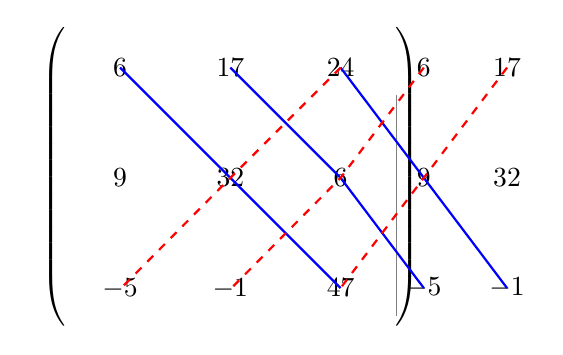
\begin{tikzpicture}[
        every node/.style={minimum size=0.7cm},
        positive/.style={blue, thick},
        negative/.style={red, thick, dashed}
    ]
    \matrix (m) [matrix of math nodes,
        nodes in empty cells,
        left delimiter=(, right delimiter=),
        column sep=0.7cm, row sep=0.7cm, % Abstand zwischen Zellen
        ampersand replacement=\&] % Wichtig für tikz-matrix
    {
        6 \& 17 \& 24  \\
        9 \& 32 \& 6   \\
        -5 \& -1 \& 47 \\
    };

    % Erweiterte Spalten (nur für die Visualisierung der Linien)
    \node at ($(m-1-3.east)!0.5!(m-1-3.east) + (0.7cm,0)$) (m-1-4) {$6$};
    \node at ($(m-2-3.east)!0.5!(m-2-3.east) + (0.7cm,0)$) (m-2-4) {$9$};
    \node at ($(m-3-3.east)!0.5!(m-3-3.east) + (0.7cm,0)$) (m-3-4) {$-5$};

    \node at ($(m-1-4.east)!0.5!(m-1-4.east) + (0.7cm,0)$) (m-1-5) {$17$};
    \node at ($(m-2-4.east)!0.5!(m-2-4.east) + (0.7cm,0)$) (m-2-5) {$32$};
    \node at ($(m-3-4.east)!0.5!(m-3-4.east) + (0.7cm,0)$) (m-3-5) {$-1$};

    % Vertikale Trennlinie (optional)
    \draw[gray, thin] ($(m-1-3.east)!0.5!(m-2-3.east) + (0.35cm,0.35cm)$) -- ($(m-3-3.east) + (0.35cm,-0.35cm)$);

    % Positive Diagonalen (blau, durchgezogen)
    \draw[positive] (m-1-1.center) -- (m-2-2.center) -- (m-3-3.center); % a-e-i
    \draw[positive] (m-1-2.center) -- (m-2-3.center) -- (m-3-4.center); % b-f-g (auf erweiterter Spalte)
    \draw[positive] (m-1-3.center) -- (m-2-4.center) -- (m-3-5.center); % c-d-h (auf erweiterter Spalte)

    % Negative Diagonalen (rot, gestrichelt)
    \draw[negative] (m-1-3.center) -- (m-2-2.center) -- (m-3-1.center); % c-e-g
    \draw[negative] (m-1-4.center) -- (m-2-3.center) -- (m-3-2.center); % a-f-h (auf erweiterter Spalte)
    \draw[negative] (m-1-5.center) -- (m-2-4.center) -- (m-3-3.center); % b-d-i (auf erweiterter Spalte)

\end{tikzpicture}

\bigskip % Etwas Abstand

Die Zahlen an den Linien werden Multipliziert. Blaue Linien werden miteinander
addiert und Rote subtrahiert.

\begin{align*}
    6 \cdot 32 \cdot 47 + 17 \cdot 6 \cdot -5 + 24 \cdot 9 \cdot -1   \\
    - -5 \cdot 32 \cdot 24 - -1 \cdot 6 \cdot 6 - 47 \cdot 9 \cdot 17 \\
    = 4983
\end{align*}

\subsubsection*{Leibniz-Formel}

Muss ich nachher machen

\subsubsection*{Kästchenregel}

\begin{longtable}{p{10cm}}
    \hline
    \multicolumn{1}{c}{\textbf{Linearkombination}}                                         \\
    \hline
    \endfirsthead

    \hline
    \multicolumn{1}{c}{\tablename\ \thetable\ -- \textit{Fortführung von vorherier Seite}} \\
    \hline
    \multicolumn{1}{c}{\textbf{Linearkombination}}                                         \\
    \hline
    \endhead

    \hline
    \multicolumn{1}{r}{\textit{Fortsetzung siehe nächste Seite}}                           \\
    \endfoot

    \hline
    \endlastfoot

    $\displaystyle\begin{matrix}
                          6  & 17 & 24 \\
                          9  & 32 & 6  \\
                          -5 & -1 & 47
                      \end{matrix}$                                                            \\\hline
    Operation: III + $\frac{5}{6}$I                                                        \\\hline\pagebreak[0]

    $\displaystyle\begin{matrix}
                          6 & 17           & 24 \\
                          9 & 32           & 6  \\
                          0 & \frac{79}{6} & 67
                      \end{matrix}$                                                    \\\hline

    Operation: II - $\frac{3}{2}$I                                                         \\\hline\pagebreak[0]

    $\displaystyle\begin{matrix}
                          6 & 17           & 24  \\
                          0 & \frac{13}{2} & -30 \\
                          0 & \frac{79}{6} & 67
                      \end{matrix}$                                                   \\\hline

\end{longtable}

\begin{align*}
    6 \cdot \det\left(\begin{pmatrix}
                              \frac{13}{2} & -30 \\ \frac{79}{6} & 67
                          \end{pmatrix}\right) \\
    = 6 \cdot \frac{13}{2} \cdot 67 - \frac{79}{6} \cdot -30 \\
    = 4983
\end{align*}

\subsection{b}

Sei $B = \begin{pmatrix}
        1 & 0 & 2 & 0 \\ 1 & 2 & 9 & 0 \\ 2 & 0 & 1 & 5 \\ 1 & 1 & 1 & 1
    \end{pmatrix}$.

Bestimmen Sie $det(B)$

\begin{longtable}{p{10cm}}

    \hline
    \multicolumn{1}{c}{\textbf{Linearkombination}}                                         \\
    \hline
    \endfirsthead

    \hline
    \multicolumn{1}{c}{\tablename\ \thetable\ -- \textit{Fortführung von vorherier Seite}} \\
    \hline
    \multicolumn{1}{c}{\textbf{Linearkombination}}                                         \\
    \hline
    \endhead

    \hline
    \multicolumn{1}{r}{\textit{Fortsetzung siehe nächste Seite}}                           \\
    \endfoot

    \hline
    \endlastfoot

    $\displaystyle\begin{matrix}
                          1 & 0 & 2 & 0 \\
                          1 & 2 & 9 & 0 \\
                          2 & 0 & 1 & 5 \\
                          1 & 1 & 1 & 1
                      \end{matrix}$                                                            \\\hline
    I und IV tauschen                                                                      \\\hline\pagebreak[0]

    $\displaystyle\begin{matrix}
                          1 & 1 & 1 & 1 \\
                          1 & 2 & 9 & 0 \\
                          2 & 0 & 1 & 5 \\
                          1 & 0 & 2 & 0
                      \end{matrix}$                                                            \\\hline
    IV - 2I                                                                                \\\hline\pagebreak[0]

    $\displaystyle\begin{matrix}
                          1  & 1 & 1 & 1  \\
                          -1 & 0 & 7 & -2 \\
                          2  & 0 & 1 & 5  \\
                          1  & 0 & 2 & 0
                      \end{matrix}$                                                          \\\hline

    IV + II                                                                                \\\hline\pagebreak[0]

    $\displaystyle\begin{matrix}
                          1  & 1 & 1 & 1  \\
                          -1 & 0 & 7 & -2 \\
                          2  & 0 & 1 & 5  \\
                          0  & 0 & 9 & -2
                      \end{matrix}$                                                          \\\hline

    III + 2II                                                                              \\\hline\pagebreak[0]

    $\displaystyle\begin{matrix}
                          1  & 1 & 1  & 1  \\
                          -1 & 0 & 7  & -2 \\
                          0  & 0 & 15 & 1  \\
                          0  & 0 & 9  & -2
                      \end{matrix}$                                                         \\\hline

\end{longtable}

\[
    B = \left( \begin{array}{cc|cc}
            1  & 1 & 1  & 1  \\
            -1 & 0 & 7  & -2 \\
            \hline
            0  & 0 & 15 & 1  \\
            0  & 0 & 9  & -2
        \end{array} \right)
    = \begin{pmatrix} A & B \\ 0 & D \end{pmatrix}
\]

wobei $A = \begin{pmatrix} 1 & 1 \\ -1 & 0 \end{pmatrix}$ und $D = \begin{pmatrix} 15 & 1 \\ 9 & -2 \end{pmatrix}$.
Die Determinante ist $\det(M) = \det(A) \cdot \det(D)$.

\bigskip

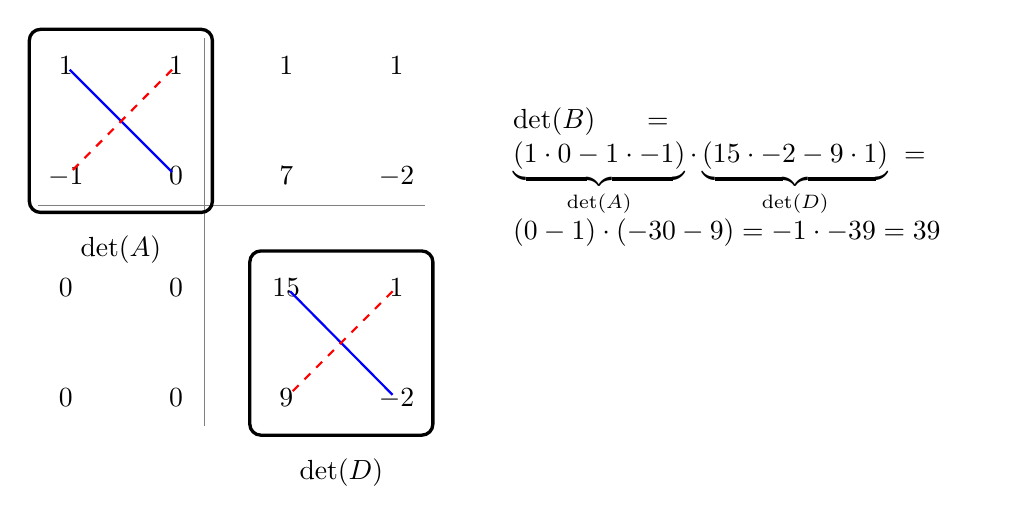
\begin{tikzpicture}[
        every node/.style={minimum size=0.7cm},
        positive/.style={blue, thick},
        negative/.style={red, thick, dashed},
        block/.style={draw, very thick, rounded corners, inner sep=3pt}
    ]
    \matrix (m) [matrix of math nodes,
        nodes in empty cells,
        column sep=0.7cm, row sep=0.7cm,
        ampersand replacement=\&]
    {
        1 \& 1 \& 1 \& 1   \\
        -1 \& 0 \& 7 \& -2 \\
        0 \& 0 \& 15 \& 1  \\
        0 \& 0 \& 9 \& -2  \\
    };

    \draw[gray, thin] (m-2-1.south west) -- (m-2-4.south east);
    \draw[gray, thin] (m-1-2.north east) -- (m-4-2.south east);

    \node[block, fit=(m-1-1) (m-2-2), label={[yshift=-0.1cm]below:$\det(A)$}] (blockA) {};
    \node[block, fit=(m-3-3) (m-4-4), label={[yshift=-0.1cm]below:$\det(D)$}] (blockD) {};

    \draw[positive, shorten >=2pt, shorten <=2pt] (m-1-1.center) -- (m-2-2.center);
    \draw[negative, shorten >=2pt, shorten <=2pt] (m-1-2.center) -- (m-2-1.center);

    \draw[positive, shorten >=2pt, shorten <=2pt] (m-3-3.center) -- (m-4-4.center);
    \draw[negative, shorten >=2pt, shorten <=2pt] (m-3-4.center) -- (m-4-3.center);

    \node[anchor=west, text width=6cm, at={($(m-2-4.east)+(1cm,0)$)}] (formel)
    {
        $\det(B) = \underbrace{(1 \cdot 0 - 1 \cdot -1)}_{\det(A)} \cdot \underbrace{(15 \cdot -2 - 9 \cdot 1)}_{\det(D)} = (0 - 1) \cdot (-30 - 9) = -1 \cdot -39 = 39$
    };
\end{tikzpicture}

\subsection{c}
Sei $C = \begin{pmatrix}
        1 & 0 & 2 & 0 \\ 1 & 2 & 9 & 0 \\ 2 & 0 & 1 & 5 \\ 1 & 2 & 9 & 0
    \end{pmatrix}$.

Bestimmen Sie ohne Rechung $det(C)$.

Die Matrix ist Linear abhängig. Daher ist die Determinante = 0.

\section{Aufgabe 3}

\subsection{a}
Prüfen Sie die Vektoren $\begin{pmatrix}5 \\ 1 \\ 9\end{pmatrix}, \begin{pmatrix}1 \\2 \\ 3\end{pmatrix}$ und $\begin{pmatrix}4 \\ 4 \\ 1\end{pmatrix}$ auf lineare Unabhängigkeit.

\begin{align*}
    det\left(\begin{pmatrix}
                 5 & 1 & 4 \\
                 1 & 2 & 4 \\
                 9 & 3 & 1
             \end{pmatrix}\right)                               \\
    =5 \cdot 2 \cdot 1 + 1 \cdot 4 \cdot 9 + 4 \cdot 1 \cdot 3  \\
    - 9 \cdot 2 \cdot 4 - 3 \cdot 4 \cdot 5 - 1 \cdot 1 \cdot 1 \\
    = 10 + 36 + 12 - 72 - 60 - 1                                \\
    = -75
\end{align*}

\subsection{b}
Ist das lineare Gleichungssystem $Ax = b$ mit $b = \begin{pmatrix}5 \\ 10 \\ 1\end{pmatrix}$ und $A = \begin{pmatrix}1 & 0 & 2 \\ 1 & 2 & 0 \\ 2 & 0 & 1\end{pmatrix}$ eindeutig lösbar?

\begin{align*}
    \det \left(\begin{pmatrix}
                   1 & 0 & 2 \\
                   1 & 2 & 0 \\
                   2 & 0 & 1
               \end{pmatrix}\right)                             \\
    = 1 \cdot 2 \cdot 1 + 0 \cdot 0 \cdot 2 + 2 \cdot 1 \cdot 0 \\
    - 2 \cdot 2 \cdot 2 - 0 \cdot 0 \cdot 1 - 1 \cdot 1 \cdot 0 \\
    = 2 + 0 + 0 - 8 - 0 - 0                                     \\
    = -6
\end{align*}

Da die Matrix Linear unabhängig ist, ist das Gleichungssystem eindeutig lösbar.
	\chapter{Übungsblatt 9}

\section{Aufgabe 1}

\subsection{a}
Seien die Geraden $G_1$ und $G_2$ definiert durch:
\begin{align*}
    G_1 & := \left\{\begin{pmatrix}
                        1 \\ 2 \\ 3
                    \end{pmatrix} + \lambda \begin{pmatrix}
                                                1 \\ 1 \\ 1
                                            \end{pmatrix}: \lambda \in \mathbb{R}\right\} \\
    G_2 & := \left\{\begin{pmatrix}
                        3 \\ 3 \\ 3
                    \end{pmatrix} + \mu \begin{pmatrix}
                                            1 \\ 1 \\ 1
                                        \end{pmatrix}: \mu \in \mathbb{R}\right\}
\end{align*}
Wie liegen $G_1$ und $G_2$ zueinander im Raum? Bestimmen Sie, je nach Lage, Schnittpunkt oder Abstand der beiden Geraden.

Da beide Vektoren die selben Richtungsvektoren besitzen, sind sie entweder echt
parallel oder identisch. Um zu prüfen, ob die beiden Vektoren Identisch sind,
muss das Gleichungssystem $G_1 = G_2 + \mu \begin{pmatrix}
        1 \\ 1 \\ 1
    \end{pmatrix}$ gelöst werden.

\begin{align*}
    \begin{pmatrix}
        1 \\ 2 \\ 3
    \end{pmatrix} = \begin{pmatrix}
                        3 \\ 3 \\ 3
                    \end{pmatrix} + \mu \cdot \begin{pmatrix}
                                                  1 \\ 1 \\ 1
                                              \end{pmatrix} \\
    \begin{cases}
        \text{I:\@}   & 1 = 3 + \mu \quad | -3 \Leftrightarrow -2 = \mu \\
        \text{II:\@}  & 2 = 3 + \mu \quad | -3 \Leftrightarrow -1 = \mu \\
        \text{III:\@} & 3 = 3 + \mu \quad | -3 \Leftrightarrow 0 = \mu
    \end{cases}
\end{align*}

Da das resultierende Gleichungssystem nicht lösbar ist, sind die Vektoren nicht
identisch. Nun muss geprüft werden, ob sie echt parallel zueinander stehen.
Hierfür muss der Abstand $d$ der Vektoren $G_1: r = p_1 + \lambda u$ und $G_2:
    r = p_2 + \mu u$ bestimmt werden, welcher sich über die Formel $d = \frac{|(p_2
        - p_1) \times u|}{|u|}$ berechnen lässt.

\begin{align*}
    d = \frac{\left|\left(p_2 - p_1\right) \times u\right|}{\left|u\right|}                                             \\
    d = \frac{\left|\left(\begin{pmatrix}
                                  3 \\ 3 \\ 3
                              \end{pmatrix} - \begin{pmatrix}
                                                  1 \\ 2 \\ 3
                                              \end{pmatrix}\right) \times \begin{pmatrix}
                                                                              1 \\ 1 \\ 1
                                                                          \end{pmatrix}\right|}{\left|\begin{pmatrix}
                                                                                                          1 \\ 1 \\ 1
                                                                                                      \end{pmatrix}\right|} \\
    d = \frac{\left|\begin{pmatrix}
                            2 \\ 1 \\ 0
                        \end{pmatrix} \times \begin{pmatrix}
                                                 1 \\ 1 \\ 1
                                             \end{pmatrix}\right|}{\left|\begin{pmatrix}
                                                                             1 \\ 1 \\ 1
                                                                         \end{pmatrix}\right|}                              \\
    d = \frac{\left|\begin{pmatrix}
                            1 \\ -2 \\ 1
                        \end{pmatrix}\right|}{\left|\begin{pmatrix}
                                                        1 \\ 1 \\ 1
                                                    \end{pmatrix}\right|}                                                   \\
    d = \frac{\sqrt{6}}{\sqrt{3}}                                                                                       \\
    d = \sqrt{2}                                                                                                        \\
\end{align*}

Der Abstand zwischen den beiden Vektoren beträgt $\sqrt{2}$. Das bedeutet, dass
diese echt parallel zueinander sind.

\subsection{b}

Es sei $E$ definiert durch:
\begin{align*}
    E := \left\{\begin{pmatrix}
                    1 \\ 0 \\1
                \end{pmatrix} + \lambda \begin{pmatrix}
                                            1 \\ 1 \\ 1
                                        \end{pmatrix} + \mu \begin{pmatrix}
                                                                2 \\ 3 \\ 4
                                                            \end{pmatrix}: \lambda, \mu \in \mathbb{R}\right\}
\end{align*}
Geben Sie $E$ in Normalenform an.

Nicht Klausurrelevant?

\section{Aufgabe 2 - nicht klausurrelevant?}

\subsection{a}
Sei $v = \begin{pmatrix}
        1 \\ 1 \\ 0
    \end{pmatrix}$ und $w = \begin{pmatrix}
        1 \\ 1 \\ 0
    \end{pmatrix}$ und $G := \left\{\lambda w: \lambda \in \mathbb{R}\right\}$. Bestimmen Sie die Projektion $v_w$ von
$v$ auf die von $w$ aufgespannte Gerade $G$.
Bestimmen Sie weiterhin die Matrix, die die lineare Abbildung $P: \mathbb{R}^3 \rightarrow G, a \mapsto aw$ dastellt.
Was ist der Rang dieser Matrix? Was ist ihr Kern? Was ihr Bild?

\subsection{b}
(Transferfrage) Sei $E := \left\{\lambda\begin{pmatrix}
        1 \\ 0 \\ 1
    \end{pmatrix} + \mu \begin{pmatrix}
        1 \\ 1 \\ 0
    \end{pmatrix}: \lambda \in \mathbb{R}\right\}$. Sei $v := \begin{pmatrix}
        1 \\ 1 \\ 2
    \end{pmatrix}$. Wie kann man die orthogonale Projektion von $v$ auf $E$ bestimmen? Welcher Vektor kommt dabei heraus?

\section{Aufgabe 3}

\subsection{a}
Sei $D_\pi: \mathbb{R}^2 \rightarrow \mathbb{R}^2$ die lineare Abbildung, die
jeden Vektor aus $\mathbb{R}^2$ um $\pi$ dreht. Sei $v := \begin{pmatrix}1 \\2\end{pmatrix}$. Sellen Sie die Matrix zu $D_\pi$ auf und bestimmen Sie
$D_\pi(v)$. Bestimmen Sie $\langle v, D_\pi(v)\rangle$.

Die 2x2 Matrix zur Drehung ist $D_\alpha = \begin{pmatrix}
        cos(\alpha) & -sin(\alpha) \\ sin(\alpha) & cos(\alpha)
    \end{pmatrix}$. Die Drehmatrix, welche um $\pi$ dreht, ist somit $D_\pi = \begin{pmatrix}
        cos(\pi) & -sin(\pi) \\ sin(\pi) & \cos(\pi)
    \end{pmatrix} = \begin{pmatrix}
        -1 & 0 \\ 0 & -1
    \end{pmatrix}$.

\begin{align*}
    D_\pi \cdot \begin{pmatrix}
                    1 \\ 2
                \end{pmatrix}                          \\
    = \begin{pmatrix}
          -1 & 0 \\ 0 & -1
      \end{pmatrix} \cdot \begin{pmatrix}
                              1 \\ 2
                          \end{pmatrix}                \\
    = \begin{pmatrix}
          -1 \cdot 1 + 0 \cdot 2 \\ 0 \cdot 1 + (-1) \cdot 2
      \end{pmatrix} \\
    = \begin{pmatrix}
          -1 \\ -2
      \end{pmatrix}
\end{align*}

\begin{align*}
    \left\langle v, D_\pi(v) \right\rangle                    \\
    = \left\langle \begin{pmatrix}
                       1 \\ 2
                   \end{pmatrix}, \begin{pmatrix}
                                      -1 \\ -2
                                  \end{pmatrix} \right\rangle \\
    = 1 \cdot -1 + 2 \cdot -2                                 \\
    = -1 + (-4)                                               \\
    = -5
\end{align*}

\subsection{b}
Sei $D : \mathbb{R}^3 \rightarrow \mathbb{R}^3$ die Drehung, die den Vektor
$(1, 0, 0)^t$ auf den Vektor $\frac{1}{\sqrt{3}}(1, 1, 1)$ abbildet. Bestimmen
Sie die Drehmatrix, die D darstellt.

\begin{align*}
    D = \begin{pmatrix}
            c_1 & c_2 & c_3 \\
            c_1 & c_2 & c_3 \\
            c_1 & c_2 & c_3
        \end{pmatrix}                                                                                                                                     \\
    D\begin{pmatrix}
         1 \\ 0 \\ 0
     \end{pmatrix}                                                                                                                                         \\
    = \frac{1}{\sqrt{3}} \begin{pmatrix}
                             1 \\ 1 \\ 1
                         \end{pmatrix}                                                                                                                     \\
    = \begin{pmatrix}
          c_1 \\ c_1 \\ c_1
      \end{pmatrix}                                                                                                                                      \\\\
    \text{Erste Bedingung an } c_2                                                                                                                          \\
    \left\langle c_1, c_2 \right\rangle = 0                                                                                                                 \\
    \left\langle \begin{pmatrix}
                     \frac{1}{\sqrt{3}} \\
                     \frac{1}{\sqrt{3}} \\
                     \frac{1}{\sqrt{3}}
                 \end{pmatrix}, \begin{pmatrix}
                                    x_1 \\ x_2 \\ x_3
                                \end{pmatrix} \right\rangle = 0                                                                                             \\
    \frac{1}{\sqrt{3}}x_1 + \frac{1}{\sqrt{3}}x_2 + \frac{1}{\sqrt{3}}x_3 = 0 \quad \frac{1}{\sqrt{3}}                                                      \\
    x_1 + x_2 + x_3 = 0                                                                                                                                     \\\\
    \text{Zweite Bedingung an } c_2                                                                                                                         \\
    \left|c_2\right| = 1                                                                                                                                    \\
    \left|\begin{pmatrix}
              x_1 \\x_2 \\ x_3
          \end{pmatrix}\right| = 1                                                                                                                          \\
    x_1^2 + x_2^2 + x_3^2 = 1                                                                                                                               \\\\
    \text{Wähle } x_3 = 0                                                                                                                                   \\
    \text{In erste Bedingung einsetzen}                                                                                                                     \\
    x_1 + x_2 + 0 = 0 \quad | - x_2                                                                                                                         \\
    \Leftrightarrow x_1 = -x_2                                                                                                                              \\\\
    \text{In zweite Bedingung einsetzen}                                                                                                                    \\
    x_1^2 + (- x_1^2) + 0^2 = 1                                                                                                                             \\
    x_1^2 + x_1^2 = 1                                                                                                                                       \\
    2x_1^2 = 1 \quad | : 2                                                                                                                                  \\
    \Leftrightarrow x_1^2 = \frac{1}{2} \quad | \sqrt{}                                                                                                     \\
    \Leftrightarrow x_1 = \frac{1}{\sqrt{2}}                                                                                                                \\
    x_2 = -x_1                                                                                                                                              \\
    x_2 = -\frac{1}{\sqrt{2}}                                                                                                                               \\
    c_2 = \begin{pmatrix}
              \frac{1}{\sqrt{2}}   \\
              - \frac{1}{\sqrt{2}} \\
              0                    \\
          \end{pmatrix}                                                                                                                \\\\
    c_3 = c_1 \times c_2                                                                                                                                    \\
    c_3 = \begin{pmatrix}
              \frac{1}{\sqrt{3}} \\
              \frac{1}{\sqrt{3}} \\
              \frac{1}{\sqrt{3}}
          \end{pmatrix} \times \begin{pmatrix}
                                   \frac{1}{\sqrt{2}} \\ -\frac{1}{\sqrt{2}} \\ 0
                               \end{pmatrix}                                                    \\
    c_3 = \begin{pmatrix}
              \frac{1}{\sqrt{3}} \cdot 0 - \frac{1}{\sqrt{3}} \cdot -\frac{1}{\sqrt{2}} \\
              \frac{1}{\sqrt{3}} \cdot \frac{1}{\sqrt{2}} - \frac{1}{\sqrt{3}} \cdot 0  \\
              \frac{1}{\sqrt{3}} \cdot -\frac{1}{\sqrt{2}} - \frac{1}{\sqrt{3}} \cdot \frac{1}{\sqrt{2}}
          \end{pmatrix} \\
    c_3 = \begin{pmatrix}
              \frac{\sqrt{6}}{6} \\ \frac{\sqrt{6}}{6} \\ -\frac{\sqrt{6}}{3}
          \end{pmatrix}                                          \\\\D = \begin{pmatrix}
        \frac{1}{\sqrt{3}} & \frac{1}{\sqrt{2}}  & \frac{\sqrt{6}}{6}  \\
        \frac{1}{\sqrt{3}} & -\frac{1}{\sqrt{2}} & \frac{\sqrt{6}}{6}  \\
        \frac{1}{\sqrt{3}} & 0                   & -\frac{\sqrt{6}}{3} \\
    \end{pmatrix}
\end{align*}

\subsection{c}

Sei $\varphi \in [0, 2\pi)$. Bestimmen Sie für die Drehmatrix $A_\varphi \in
    \mathbb{R}^{2 \times 2}$ und $A_{3, \varphi} \in \mathbb{R}^{3 \times 3}$
(Drehung um die $x_3$-Achse) die Determinante. Bestimmen Sie weiterhin das
Produkt $A^t_\varphi A^t_\varphi$ bzw. $A^t_{3, \varphi} A_{3, \varphi}$. Was
ist also die Inverse $A^{-1}_{\varphi}$ bzw. $A^{-1}_{3, \varphi}$?


	\chapter{Übungsblatt 10}

\section{Aufgabe 1}

Bestimmen Sie sämtliche Eigenwerte der folgenden Matrizen:

\subsection{a}

\begin{align*}
    A := \begin{pmatrix}
        1 & 2 & 3 \\
        4 & 5 & 6 \\ 
        0 & 0 & 0
    \end{pmatrix}
\end{align*}

\begin{align*}
    A - \lambda \cdot I \\
    = \begin{pmatrix}
        1 & 2 & 3 \\ 
        4 & 5 & 6 \\ 
        0 & 0 & 0
    \end{pmatrix} - \lambda \cdot \begin{pmatrix}
        1 & 0 & 0 \\
        0 & 1 & 0 \\
        0 & 0 & 1
    \end{pmatrix} \\
    = \begin{pmatrix}
        1 & 2 & 3 \\ 
        4 & 5 & 6 \\ 
        0 & 0 & 0
    \end{pmatrix}\begin{pmatrix}
        \lambda & 0 & 0 \\
        0 & \lambda & 0 \\
        0 & 0 & \lambda
    \end{pmatrix} \\
    = \begin{pmatrix}
        1 - \lambda & 2 & 3 \\
        4 & 5 - \lambda & 6 \\
        0 & 0 & -\lambda
    \end{pmatrix} =: A_\lambda \\
    \det(A_\lambda) = (1 - \lambda) \cdot (5 - \lambda) \cdot (-\lambda) \\
        + 2 \cdot 6 \cdot 0  + 3 \cdot 4 \cdot 0 - 0 \cdot (5 - \lambda) \cdot 3\\
        - 0 \cdot 6 \cdot (1 - \lambda) - (-\lambda) \cdot 4 \cdot 2 \\
    = (5 - \lambda - 5\lambda + \lambda^2) \cdot (-\lambda) + 0 \\
        + 0 - 0 - 0 + 4\lambda \cdot 2 \\
    = -5\lambda +\lambda^2 +5\lambda^2 -\lambda^3 + 8\lambda \\
    = -\lambda^3 + 6\lambda^2 + 3\lambda \\
    \text{$\lambda$ Ausklammern} \\
    \lambda (-\lambda^2 + 6\lambda + 3) \\\\
    \lambda (-\lambda^2 + 6\lambda + 3) = 0\\
    \text{Ein Produkt ist null, wenn ein Faktor gleich null ist} \\
    \begin{cases}
        \lambda = 0 & \text{Oder} \\
        -\lambda^2 + 6\lambda + 3 = 0
    \end{cases} \\
    \lambda_1 = 0 \\
    -\lambda^2 + 6 \lambda + 3 = 0 \quad |\cdot (-1) \\
    \Leftrightarrow \lambda^2 - 6 \lambda - 3 = 0 \quad | \text{PQ-Formel} \\
    p = 6 \quad q = -3 \\
    \lambda_{2,3} = -\frac{-6}{2} \pm \sqrt{\left(\frac{6}{2}\right)^2 + 3} \\
    \lambda_{2,3}= 3 \pm \sqrt{\left(3\right)^2 + 3} \\
    \lambda_{2,3}= 3 \pm \sqrt{9 + 3} \\
    \lambda_{2,3}= 3 \pm \sqrt{12} \\\\
    \lambda_1 = 0, \quad \lambda_2 = 3 + \sqrt{12}, \quad \lambda_3 = 3 - \sqrt{12}
\end{align*}

\subsection{b}

\begin{align*}
    B := \begin{pmatrix}
        1 & 1 & 1 \\
        1 & 1 & 1 \\
        1 & 1 & 1
    \end{pmatrix}
\end{align*}

\begin{align*}
    B - \lambda \cdot I \\
    \begin{pmatrix}
        1 & 1 & 1 \\
        1 & 1 & 1 \\
        1 & 1 & 1
    \end{pmatrix} - \lambda \cdot \begin{pmatrix}
        1 & 0 & 0 \\
        0 & 1 & 0 \\
        0 & 0 & 1
    \end{pmatrix} \\
        \begin{pmatrix}
        1 & 1 & 1 \\
        1 & 1 & 1 \\
        1 & 1 & 1
    \end{pmatrix} - \begin{pmatrix}
        \lambda & 0 & 0 \\
        0 & \lambda & 0 \\
        0 & 0 & \lambda
    \end{pmatrix} \\
    \begin{pmatrix}
        1 - \lambda & 1 & 1 \\
        1 & 1 - \lambda & 1 \\
        1 & 1 & 1 - \lambda
    \end{pmatrix} =: B_\lambda \\
    \det(B_\lambda) = (1 - \lambda) \cdot (1 - \lambda) \cdot (1 - \lambda) \\
                    + 1 \cdot 1 \cdot 1 + 1 \cdot 1 \cdot 1 - 1 \cdot (1 - \lambda) \cdot 1 \\
                    - 1 \cdot 1 \cdot (1 - \lambda) - (1 - \lambda) \cdot 1 \cdot 1 \\
    = (1 -\lambda - \lambda + \lambda^2) \cdot (1 - \lambda) + 1 \\
        + 1 - (1 - \lambda) - (1 - \lambda) - (1 - \lambda) \\
    = (1 - 2\lambda + \lambda^2) \cdot (1 - \lambda) + 2 - 3(1 - \lambda) \\
    = 1 - 2\lambda + \lambda^2 - \lambda + 2\lambda^2 - \lambda^3 + 2 - 3 + 3\lambda \\
    = -\lambda^3 + 3\lambda^2 \\\\
    -\lambda^3 + 3\lambda^2 = 0 \\
    \text{$\lambda$ Ausklammern} \\
    \lambda (-\lambda^2 + 3\lambda) = 0 \\
    \text{Ein Produkt ist null, wenn mindestens ein Faktor gleich null ist.} \\
    \begin{cases}
        \lambda = 0 & \text{Oder} \\
        -\lambda^2 + 3 \lambda = 0
    \end{cases} \\
    \lambda_1 = 0 \\
    \text{$\lambda$ Ausklammern} \\
    \lambda(\lambda + 3) = 0 \\
    \text{Ein Produkt ist null, wenn mindestens ein Faktor gleich null ist.} \\
    \begin{cases}
        \lambda = 0 & \text{Oder} \\
        \lambda + 3 = 0
    \end{cases} \\
    \lambda_2 = 0 \\
    \lambda_3 + 3 = 0 \quad | -3 \\
    \lambda_3 = -3 \\\\
    \lambda_1 = 0, \quad \lambda_2 = 0, \quad \lambda_3 = -3
\end{align*}

\subsection{c}

\begin{align*}
    C := \begin{pmatrix}
        0 & 0 & 0 \\
        0 & 0 & 0 \\
        0 & 0 & 0
    \end{pmatrix}
\end{align*}

\begin{align*}
    C - \lambda \cdot I \\
    \begin{pmatrix}
        0 & 0 & 0 \\
        0 & 0 & 0 \\
        0 & 0 & 0
    \end{pmatrix} - \lambda \cdot \begin{pmatrix}
        1 & 0 & 0 \\
        0 & 1 & 0 \\
        0 & 0 & 1
    \end{pmatrix} \\
    \begin{pmatrix}
        0 & 0 & 0 \\
        0 & 0 & 0 \\
        0 & 0 & 0
    \end{pmatrix} - \begin{pmatrix}
        \lambda & 0 & 0 \\
        0 & \lambda & 0 \\
        0 & 0 & \lambda
    \end{pmatrix} \\
    \begin{pmatrix}
        -\lambda & 0 & 0 \\
        0 & -\lambda & 0 \\
        0 & 0 & -\lambda
    \end{pmatrix} =: C_\lambda \\
    \det(C_\lambda) = -\lambda \cdot -\lambda \cdot -\lambda \\
    = -\lambda^3 \\\\
    -\lambda^3 = 0 \quad |\cdot (-1) \\
    \Leftrightarrow \lambda^3 = 0 \quad | \sqrt[3]{0} \\
    \Leftrightarrow \lambda_{1, 2, 3} = 0
\end{align*}

\subsection{d}

\begin{align*}
    D := \begin{pmatrix}
        0 & 1 \\
        2 & 3
    \end{pmatrix}
\end{align*}

\begin{align*}
    D - \lambda \cdot I \\
        \begin{pmatrix}
        0 & 1 \\
        2 & 3
    \end{pmatrix} - \lambda \cdot \begin{pmatrix}
        1 & 0 \\
        0 & 1
    \end{pmatrix} \\
    \begin{pmatrix}
        0 & 1 \\
        2 & 3
    \end{pmatrix} - \begin{pmatrix}
        \lambda & 0 \\
        0 & \lambda
    \end{pmatrix} \\
    \begin{pmatrix}
        -\lambda & 1 \\
        2 & 3 - \lambda
    \end{pmatrix} =: D_\lambda\\\\
    \det(D_\lambda) = -\lambda \cdot (3 - \lambda) - 2 \cdot 1 \\
    = \lambda^2 - 3 \lambda - 2 \\\\
    \lambda^2 - 3 \lambda - 2 = 0 \quad | PQ\\
    p = -3 \quad q = -2 \\
    -\frac{-3}{2} \pm \sqrt{\left(\frac{-3}{2}\right)^2 + 2} \\
    \frac{3}{2} \pm \sqrt{\left(\frac{9}{4}\right) + 2} \\
    \frac{3}{2} \pm \sqrt{\frac{17}{4}} \\
    \lambda_1 = \frac{3}{2} + \sqrt{\frac{17}{4}}, \quad \lambda_2 = \frac{3}{2} - \sqrt{\frac{17}{4}}
\end{align*}

\section{Aufgabe 2}

\subsection{a}

Ist die Matrix $A := \begin{pmatrix}
    1 & 2 & 3 \\
    4 & 5 & 6 \\
    7 & 8 & 9
\end{pmatrix}$ positiv definit?

\begin{align*}
    \det(\Delta_1) = 1 \\
    \det(\Delta_2) = 1 \cdot 5 - 2 \cdot 4 = -3 \\
\end{align*}

Die Determinante des dritten Hauptminoren ist hier uninteressant, da die Vorzeichenfolge für positive definitheit durch den zweiten Hauptminoren bereits verletzt wurde. Die Matrix ist \textit{nicht} positiv definit, sondern Indefinit.

\subsection{b}
Wie kann man das Hauptminorenkriterium nutzen, um zu zeigen, dass eine Matrix negativ definit ist? Nutzen Sie Ihr Ergebnis, um zu zeigen, dass die Matrix $B := \begin{pmatrix}
    -1 & 1 \\
    -2 & 1
\end{pmatrix}$ (negativ definit ist??)

\begin{align*}
    \det(\Delta_1) = -1 \\
    \det(\Delta_2) = -1 \cdot 1 - (-2) \cdot 1 = 1
\end{align*}

Die Matrix ist negativ definit.

\section{Aufgabe 3}

\subsection{a}

Für welche Winkel $\varphi \in [0, 2\pi)$ hat eine Drehmatrix $A_\varphi \in \mathbb{R}^{2 \times 2}$ reele Eigenwerte? Lösen Sie diese Aufgabe einerseits durch geometrische Argumentation, andererseits rechnerisch.

\subsubsection*{Geometrische Argumentation}

Drehmatritzen mit gerader Dimension haben keine reellen Eigenwerte. Aus diesem Grund hat nur die Drehmatrix, welche um den Winkel 0 dreht (also gar nicht dreht) reele Eigenwerte.

\subsubsection*{Rechnerisch}

\begin{align*}
    A_0 = \begin{pmatrix}
        1 & 0 \\
        0 & 1
    \end{pmatrix} \rightarrow \lambda_{1,2} = 1 \\
    \det\left(\begin{pmatrix}
        \cos(\varphi) & -\sin(\varphi) \\
        \sin(\varphi) & \cos(\varphi)
    \end{pmatrix} - \begin{pmatrix}
        \lambda & 0 \\
        0 & \lambda
    \end{pmatrix}\right) = 0 \\
    (\cos(\varphi) - \lambda) \cdot (\cos(\varphi) - \lambda) - \sin(\varphi) \cdot -\sin(\varphi) = 0 \\
    {\cos(\varphi)}^2 - \cos(\varphi) \cdot \lambda - \cos(\varphi) \cdot \lambda  + \lambda^2 + {\sin(\varphi)}^2 = 0\\
    {\cos(\varphi)}^2 + {\sin(\varphi)}^2 - 2 \cdot \cos(\varphi) \cdot \lambda + \lambda^2 = 0 \\
    1 - 2 \cdot \cos(\varphi) \cdot \lambda + \lambda^2 = 0 \quad | PQ\\
    p = - 2 \cdot \cos(\varphi), \quad q = 1 \\
    -\frac{- 2 \cdot \cos(\varphi)}{2} \pm \sqrt{\left(\frac{- 2 \cdot \cos(\varphi)}{2}\right)^2 - 1} \\
    \cos(\varphi)\pm \sqrt{(-\cos(\varphi))^2 - 1} \\
    \cos(\varphi)\pm \sqrt{\cos(\varphi)^2 - 1} \\
    \cos(\varphi)\pm \sqrt{-\sin(\varphi)^2} \\
    \text{Aus negativen Zahlen kann die Wurzel nicht gezogen werden.} \\
    \text{Für alle } \varphi \neq 0 \text{ Gibt es keine reellen lösungen.}
\end{align*}

\subsection{b}

Bestimmen Sie mindestens eine Matrix, die in $O(n) \backslash SO(n)$ enthalten ist.

\begin{align*}
    \begin{pmatrix}
        0 & 1 \\
        1 & 0
    \end{pmatrix} \\
    \det\left(    \begin{pmatrix}
        0 & 1 \\
        1 & 0
    \end{pmatrix}\right) = -1 \\
\end{align*}
	\chapter{Übungsblatt 11}

\section{Aufgabe 1}
Bestimmen Sie jeweilts sämtliche Eigenvektoren der folgenden Matzitzen.
Hinweis: Die Eigenwerte haben Sie bereits auf dem letzten Übungsblatt bestimmt:

\subsection{a}

\begin{align*}
    A := \begin{pmatrix}
             1 & 2 & 3 \\
             4 & 5 & 6 \\
             0 & 0 & 0
         \end{pmatrix}                                                             \\
    \lambda_1 = 0, \quad \lambda_2 = 3 + \sqrt{12}, \quad \lambda_3 = 3 - \sqrt{12} \\
    \begin{pmatrix}
        1 - \lambda & 2           & 3        \\
        4           & 5 - \lambda & 6        \\
        0           & 0           & -\lambda
    \end{pmatrix}                                            \\\\
    \text{Für } \lambda_1 = 0                                                       \\
    \begin{pmatrix}
        1 - 0 & 2     & 3     \\
        4     & 5 - 0 & 6     \\
        0     & 0     & 0 - 0
    \end{pmatrix}                                                           \\
    \begin{pmatrix}
        1 & 2 & 3 \\
        4 & 5 & 6 \\
        0 & 0 & 0
    \end{pmatrix}                                                                  \\
    \begin{pmatrix}
        1 & 2 & 3 \\
        4 & 5 & 6 \\
        0 & 0 & 0
    \end{pmatrix} \cdot \begin{pmatrix}
                            x_1 \\ x_2 \\ x_3
                        \end{pmatrix} = \begin{pmatrix}
                                            0 \\ 0 \\ 0
                                        \end{pmatrix}                              \\
    \begin{cases}
        \text{I:\@}   & 1 \cdot x_1 + 2 \cdot x_2 + 3 \cdot x_3 = 0 \\
        \text{II:\@}  & 4 \cdot x_1 + 5 \cdot x_2 + 6 \cdot x_3 = 0 \\
        \text{III:\@} & 0 \cdot x_1 + 0 \cdot x_2 + 0 \cdot x_3 = 0
    \end{cases}                     \\
    \begin{cases}
        \text{I:\@}   & 1x_1 + 2x_2 + 3x_3 = 0 \\
        \text{II:\@}  & 4x_1 + 5x_2 + 6x_3 = 0 \\
        \text{III:\@} & 0 = 0
    \end{cases}
\end{align*}

\begin{longtable}{p{10cm}}
    \hline
    \multicolumn{1}{c}{\textbf{Linearkombination}}                                         \\
    \hline
    \endfirsthead

    \hline
    \multicolumn{1}{c}{\tablename\ \thetable\ -- \textit{Fortführung von vorherier Seite}} \\
    \hline
    \multicolumn{1}{c}{\textbf{Linearkombination}}                                         \\
    \hline
    \endhead

    \hline
    \multicolumn{1}{r}{\textit{Fortsetzung siehe nächste Seite}}                           \\
    \endfoot

    \hline
    \endlastfoot

    $\displaystyle\begin{matrix}
                          1 & 2 & 3 \\
                          4 & 5 & 6
                      \end{matrix}$                                                            \\\hline
    II - 2I                                                                                \\\hline\pagebreak[0]
    $\displaystyle\begin{matrix}
                          1 & 2 & 3 \\
                          2 & 1 & 0
                      \end{matrix}$                                                            \\\hline
    I - 2II                                                                                \\\hline\pagebreak[0]
    $\displaystyle\begin{matrix}
                          -3 & 0 & 3 \\
                          2  & 1 & 0
                      \end{matrix}$                                                            \\\hline
    I : (-3)                                                                               \\\hline\pagebreak[0]
    $\displaystyle\begin{matrix}
                          1 & 0 & -1 \\
                          2 & 1 & 0
                      \end{matrix}$                                                            \\\hline
    II - 2I                                                                                \\\hline\pagebreak[0]
    $\displaystyle\begin{matrix}
                          1 & 0 & -1 \\
                          0 & 1 & -2
                      \end{matrix}$                                                            \\\hline
\end{longtable}

\begin{align*}
    \begin{cases}
        \text{I:\@}  & x_1 - x_3 = 0 \quad | + x_3 \Leftrightarrow x_1 = x_3   \\
        \text{II:\@} & x_2 - 2x_3 = 0 \quad | +2x_3 \Leftrightarrow x_2 = 2x_3
    \end{cases} \\
    x_3 = t, \text{ mit } t \in \mathbb{R}                                 \\
    \begin{pmatrix}
        t \\ 2t \\ t
    \end{pmatrix}                                                         \\
    L = \left\{t \cdot \begin{pmatrix}
                           1 \\ 2 \\ 1
                       \end{pmatrix}\right\}                               \\
    span = \left\{\begin{pmatrix}
                      1 \\ 2 \\ 1
                  \end{pmatrix}\right\}
\end{align*}

\begin{align*}
    \text{Für } \lambda_2 = 3 + \sqrt{12}                           \\
    \begin{pmatrix}
        1 - \lambda & 2           & 3           \\
        4           & 5 - \lambda & 6           \\
        0           & 0           & 0 - \lambda
    \end{pmatrix}                         \\
    \begin{pmatrix}
        1 - (3 + \sqrt{12}) & 2                   & 3                   \\
        4                   & 5 - (3 + \sqrt{12}) & 6                   \\
        0                   & 0                   & 0 - (3 + \sqrt{12})
    \end{pmatrix} \\
    \begin{pmatrix}
        1 - 3 - \sqrt{12} & 2                 & 3                 \\
        4                 & 5 - 3 - \sqrt{12} & 6                 \\
        0                 & 0                 & 0 - 3 - \sqrt{12}
    \end{pmatrix}       \\
    \begin{pmatrix}
        -2 - \sqrt{12} & 2             & 3              \\
        4              & 2 - \sqrt{12} & 6              \\
        0              & 0             & -3 - \sqrt{12}
    \end{pmatrix}                 \\
    \begin{pmatrix}
        -2 - \sqrt{12} & 2             & 3              \\
        4              & 2 - \sqrt{12} & 6              \\
        0              & 0             & -3 - \sqrt{12}
    \end{pmatrix} \cdot \begin{pmatrix}
                            x_1 \\ x_2 \\ x_3
                        \end{pmatrix} = \begin{pmatrix}
                                            0 \\ 0 \\ 0
                                        \end{pmatrix}              \\
    \begin{cases}
        \text{I:\@}   & (-2 - \sqrt{12})x_1 + 2x_2 + 3x_3 = 0 \\
        \text{II:\@}  & 4x_1 + (2 - \sqrt{12})x_2 + 6x_3 = 0  \\
        \text{III:\@} & 0x_1 + 0x_2 + (-3 - \sqrt{12})x_3 = 0
    \end{cases}
\end{align*}

\begin{longtable}{p{10cm}}
    \hline
    \multicolumn{1}{c}{\textbf{Linearkombination}}                                         \\
    \hline
    \endfirsthead

    \hline
    \multicolumn{1}{c}{\tablename\ \thetable\ -- \textit{Fortführung von vorherier Seite}} \\
    \hline
    \multicolumn{1}{c}{\textbf{Linearkombination}}                                         \\
    \hline
    \endhead

    \hline
    \multicolumn{1}{r}{\textit{Fortsetzung siehe nächste Seite}}                           \\
    \endfoot

    \hline
    \endlastfoot

    $\displaystyle\begin{matrix}
                          -2 - \sqrt{12} & 2             & 3              \\
                          4              & 2 - \sqrt{12} & 6              \\
                          0              & 0             & -3 - \sqrt{12}
                      \end{matrix}$                          \\\hline
    III : (-3 - $\sqrt{12}$)                                                               \\\hline\pagebreak[0]
    $\displaystyle\begin{matrix}
                          -2 - \sqrt{12} & 2             & 3 \\
                          4              & 2 - \sqrt{12} & 6 \\
                          0              & 0             & 1
                      \end{matrix}$                                       \\\hline
    (-2 - $\sqrt{12}$)II - 4I                                                              \\\hline\pagebreak[0]
    $\displaystyle\begin{matrix}
                          -2 - \sqrt{12} & 2 & 3                \\
                          0              & 0 & -24 - 12\sqrt{3} \\
                          0              & 0 & 1
                      \end{matrix}$                                    \\\hline
    II - $(-24 - 12\sqrt{3})$III                                                           \\\hline\pagebreak[0]
    $\displaystyle\begin{matrix}
                          -2 - \sqrt{12} & 2 & 3 \\
                          0              & 0 & 0 \\
                          0              & 0 & 1
                      \end{matrix}$                                                   \\\hline
    I - 3III                                                                               \\\hline\pagebreak[0]
    $\displaystyle\begin{matrix}
                          -2 - \sqrt{12} & 2 & 0 \\
                          0              & 0 & 0 \\
                          0              & 0 & 1
                      \end{matrix}$                                                   \\\hline
    I : (-2 - $\sqrt{12}$)                                                                 \\\hline\pagebreak[0]
    $\displaystyle\begin{matrix}
                          1 & \frac{2}{-2-\sqrt{12}} & 0 \\
                          0 & 0                      & 0 \\
                          0 & 0                      & 1
                      \end{matrix}$                              \\\hline

\end{longtable}

\begin{align*}
    x_2 = t, \text{ mit } t \in \mathbb{R}                                                                                                                                    \\
    \begin{cases}
        \text{I:\@}   & x_1 + \frac{2}{-2-\sqrt{12}}t = 0 \quad | - \frac{2}{-2-\sqrt{12}}t \Leftrightarrow x_1 = -\frac{2}{-2-\sqrt{12}}t \\
        \text{II:\@}  & 0 = 0                                                                                                              \\
        \text{III:\@} & x_3 = 0
    \end{cases} \\
    \begin{pmatrix}
        -\frac{2}{-2-\sqrt{12}}t \\
        t                        \\
        0
    \end{pmatrix}                                                                                                                                     \\
    L = \left\{t \cdot \begin{pmatrix}
                           -\frac{2}{-2-\sqrt{12}} \\
                           1                       \\
                           0
                       \end{pmatrix}\right\}                                                                                                                   \\
    span = \left\{\begin{pmatrix}
                      -\frac{2}{-2-\sqrt{12}} \\
                      1                       \\
                      0
                  \end{pmatrix}\right\}
\end{align*}

\begin{align*}
    \text{Für } \lambda_3 = 3 - \sqrt{12}                           \\
    \begin{pmatrix}
        1 - \lambda & 2           & 3           \\
        4           & 5 - \lambda & 6           \\
        0           & 0           & 0 - \lambda
    \end{pmatrix}                         \\
    \begin{pmatrix}
        1 - (3 - \sqrt{12}) & 2                   & 3                   \\
        4                   & 5 - (3 - \sqrt{12}) & 6                   \\
        0                   & 0                   & 0 - (3 - \sqrt{12})
    \end{pmatrix} \\
    \begin{pmatrix}
        -2 + \sqrt{12} & 2             & 3              \\
        4              & 2 + \sqrt{12} & 6              \\
        0              & 0             & -3 + \sqrt{12}
    \end{pmatrix}                 \\
    \begin{pmatrix}
        -2 + \sqrt{12} & 2             & 3              \\
        4              & 2 + \sqrt{12} & 6              \\
        0              & 0             & -3 + \sqrt{12}
    \end{pmatrix} \cdot \begin{pmatrix}
                            x_1 \\ x_2 \\ x_3
                        \end{pmatrix} = \begin{pmatrix}
                                            0 \\ 0 \\ 0
                                        \end{pmatrix}              \\
    \begin{cases}
        \text{I:\@}   & (-2 + \sqrt{12})x_1 + 2x_2 + 3x_3 = 0 \\
        \text{II:\@}  & 4x_1 + (2 + \sqrt{12})x_2 + 6x_3 = 0  \\
        \text{III:\@} & (-3 + \sqrt{12})x_3 = 0
    \end{cases}
\end{align*}

\begin{longtable}{p{10cm}}
    \hline
    \multicolumn{1}{c}{\textbf{Linearkombination}}                                         \\
    \hline
    \endfirsthead

    \hline
    \multicolumn{1}{c}{\tablename\ \thetable\ -- \textit{Fortführung von vorherier Seite}} \\
    \hline
    \multicolumn{1}{c}{\textbf{Linearkombination}}                                         \\
    \hline
    \endhead

    \hline
    \multicolumn{1}{r}{\textit{Fortsetzung siehe nächste Seite}}                           \\
    \endfoot

    \hline
    \endlastfoot

    $\displaystyle\begin{matrix}
                          -2 + \sqrt{12} & 2             & 3              \\
                          4              & 2 + \sqrt{12} & 6              \\
                          0              & 0             & -3 + \sqrt{12}
                      \end{matrix}$                          \\\hline
    III : (-3 + $\sqrt{12}$)                                                               \\\hline\pagebreak[0]
    $\displaystyle\begin{matrix}
                          -2 + \sqrt{12} & 2             & 3 \\
                          4              & 2 + \sqrt{12} & 6 \\
                          0              & 0             & 1
                      \end{matrix}$                                       \\\hline
    I - 3III                                                                               \\\hline\pagebreak[0]
    II - 6III                                                                              \\\hline\pagebreak[0]
    $\displaystyle\begin{matrix}
                          -2 + \sqrt{12} & 2             & 0 \\
                          4              & 2 + \sqrt{12} & 0 \\
                          0              & 0             & 1
                      \end{matrix}$                                       \\\hline
    (-2 + $\sqrt{12}$)II - 4I                                                              \\\hline\pagebreak[0]
    $\displaystyle\begin{matrix}
                          -2 + \sqrt{12} & 2 & 0 \\
                          0              & 0 & 0 \\
                          0              & 0 & 1
                      \end{matrix}$                                                   \\\hline
    I : (-2 + $\sqrt{12}$)                                                                 \\\hline\pagebreak[0]
    $\displaystyle\begin{matrix}
                          1 & \frac{2}{-2 + \sqrt{12}} & 0 \\
                          0 & 0                        & 0 \\
                          0 & 0                        & 1
                      \end{matrix}$                            \\

\end{longtable}

\begin{align*}
    \begin{cases}
        \text{I:\@}   & x_1 + \frac{2}{-2 + \sqrt{12}}x_2 = 0 \quad |- \frac{2}{-2 + \sqrt{12}}x_2 \Leftrightarrow x_1 =  \frac{-1+\sqrt{3}}{2}x_2 \\
        \text{II:\@}  & 0 = 0                                                                                                                      \\
        \text{III:\@} & x_3 = 0
    \end{cases} \\
    x_2 = t \text{ wobei } t \in \mathbb{R}                                                                                                                                            \\
    \begin{pmatrix}
        \frac{2}{-2 + \sqrt{12}}t \\
        t                         \\
        0
    \end{pmatrix}                                                                                                                                             \\
    t \cdot \begin{pmatrix}
                \frac{2}{-2 + \sqrt{12}} \\
                1                        \\
                0
            \end{pmatrix}                                                                                                                                      \\
    span \left\{\begin{pmatrix}
                    \frac{2}{-2 + \sqrt{12}} \\
                    1                        \\
                    0
                \end{pmatrix}\right\}
\end{align*}

\subsection{b}

\begin{align*}
    B := \begin{pmatrix}
             1 & 1 & 1 \\
             1 & 1 & 1 \\
             1 & 1 & 1
         \end{pmatrix}
\end{align*}

\begin{align*}
    \lambda_1 = 0, \quad \lambda_2 = 0, \quad \lambda_3 = -3 \\
    \text{Für } \lambda_1 = \lambda_2 = 0                    \\
    \begin{pmatrix}
        1 - \lambda & 1           & 1           \\
        1           & 1 - \lambda & 1           \\
        1           & 1           & 1 - \lambda
    \end{pmatrix}                  \\
    \begin{pmatrix}
        1 - 0 & 1     & 1     \\
        1     & 1 - 0 & 1     \\
        1     & 1     & 1 - 0
    \end{pmatrix}                                    \\
    \begin{pmatrix}
        1 & 1 & 1 \\
        1 & 1 & 1 \\
        1 & 1 & 1
    \end{pmatrix}                                           \\
    \begin{pmatrix}
        1 & 1 & 1 \\
        1 & 1 & 1 \\
        1 & 1 & 1
    \end{pmatrix} \cdot \begin{pmatrix}
                            x_1 \\ x_2 \\ x_3
                        \end{pmatrix} = \begin{pmatrix}
                                            0 \\ 0 \\ 0
                                        \end{pmatrix}       \\
    \begin{cases}
        \text{I:\@}   & x_1 + x_2 + x_3 = 0 \\
        \text{II:\@}  & x_1 + x_2 + x_3 = 0 \\
        \text{III:\@} & x_1 + x_2 + x_3 = 0 \\
    \end{cases}
\end{align*}

\begin{longtable}{p{10cm}}
    \hline
    \multicolumn{1}{c}{\textbf{Linearkombination}}                                         \\
    \hline
    \endfirsthead

    \hline
    \multicolumn{1}{c}{\tablename\ \thetable\ -- \textit{Fortführung von vorherier Seite}} \\
    \hline
    \multicolumn{1}{c}{\textbf{Linearkombination}}                                         \\
    \hline
    \endhead

    \hline
    \multicolumn{1}{r}{\textit{Fortsetzung siehe nächste Seite}}                           \\
    \endfoot

    \hline
    \endlastfoot

    $\displaystyle\begin{matrix}
                          1 & 1 & 1 \\
                          1 & 1 & 1 \\
                          1 & 1 & 1
                      \end{matrix}$                                                            \\\hline
    II - I                                                                                 \\\hline\pagebreak[0]
    $\displaystyle\begin{matrix}
                          1 & 1 & 1 \\
                          0 & 0 & 0 \\
                          1 & 1 & 1
                      \end{matrix}$                                                            \\\hline
    III - I                                                                                \\\hline\pagebreak[0]
    $\displaystyle\begin{matrix}
                          1 & 1 & 1 \\
                          0 & 0 & 0 \\
                          0 & 0 & 0
                      \end{matrix}$                                                            \\\hline
\end{longtable}

\begin{align*}
    \begin{cases}
        \text{I:\@}   & x_1 + x_2 + x_3 = 0 \quad | -x_2 - x_3 \Leftrightarrow x_1 = -x_2 - x_3 \\
        \text{II:\@}  & 0 = 0                                                                   \\
        \text{III:\@} & 0 = 0
    \end{cases} \\
    x_2 = t \text{ wobei } t \in \mathbb{R}                                                 \\
    x_3 = p \text{ wobei } p \in \mathbb{R}                                                 \\
    \begin{pmatrix}
        -t -p \\ t \\ p
    \end{pmatrix}                                                                          \\
    t \begin{pmatrix}
          -1 -p \\ 1 \\ p
      \end{pmatrix}                                                                        \\
    t \begin{pmatrix}
          -1 \\ 1 \\ 0
      \end{pmatrix} + p \begin{pmatrix}
                            -1 \\ 0 \\ 1
                        \end{pmatrix}                                                      \\
    span = \left\{\begin{pmatrix}
                      -1 \\ 1 \\ 0
                  \end{pmatrix}, \begin{pmatrix}
                                     -1 \\ 0 \\ 1
                                 \end{pmatrix}\right\}
\end{align*}

\begin{align*}
    \text{Für } \lambda_3 = -3                         \\
    \begin{pmatrix}
        1 - \lambda & 1           & 1           \\
        1           & 1 - \lambda & 1           \\
        1           & 1           & 1 - \lambda
    \end{pmatrix}            \\
    \begin{pmatrix}
        1 - -3 & 1      & 1      \\
        1      & 1 - -3 & 1      \\
        1      & 1      & 1 - -3
    \end{pmatrix}                           \\
    \begin{pmatrix}
        4 & 1 & 1 \\
        1 & 4 & 1 \\
        1 & 1 & 4
    \end{pmatrix}                                     \\
    \begin{pmatrix}
        4 & 1 & 1 \\
        1 & 4 & 1 \\
        1 & 1 & 4
    \end{pmatrix} \cdot \begin{pmatrix}
                            x_1 \\ x_2 \\ x_3
                        \end{pmatrix} = \begin{pmatrix}
                                            0 \\ 0 \\ 0
                                        \end{pmatrix} \\
    \begin{cases}
        \text{I:\@}   & 4x_1 + x_2 + x_3 = 0 \\
        \text{II:\@}  & x_1 + 4x_2 + x_3 = 0 \\
        \text{III:\@} & x_1 + x_2 + 4x_3 = 0
    \end{cases}
\end{align*}

\begin{longtable}{p{10cm}}
    \hline
    \multicolumn{1}{c}{\textbf{Linearkombination}}                                         \\
    \hline
    \endfirsthead

    \hline
    \multicolumn{1}{c}{\tablename\ \thetable\ -- \textit{Fortführung von vorherier Seite}} \\
    \hline
    \multicolumn{1}{c}{\textbf{Linearkombination}}                                         \\
    \hline
    \endhead

    \hline
    \multicolumn{1}{r}{\textit{Fortsetzung siehe nächste Seite}}                           \\
    \endfoot

    \hline
    \endlastfoot

    $\displaystyle\begin{matrix}
                          4 & 1 & 1 \\
                          1 & 4 & 1 \\
                          1 & 1 & 4
                      \end{matrix}$                                                            \\\hline
    II - III                                                                               \\\hline\pagebreak[0]
    $\displaystyle\begin{matrix}
                          4 & 1 & 1  \\
                          0 & 3 & -3 \\
                          1 & 1 & 4
                      \end{matrix}$                                                            \\\hline
    4III - I                                                                               \\\hline\pagebreak[0]
    $\displaystyle\begin{matrix}
                          4 & 1  & 1   \\
                          0 & 3  & -3  \\
                          0 & -3 & -15
                      \end{matrix}$                                                            \\\hline
    III + II                                                                               \\\hline\pagebreak[0]
    $\displaystyle\begin{matrix}
                          4 & 1 & 1   \\
                          0 & 3 & -3  \\
                          0 & 0 & -18
                      \end{matrix}$                                                            \\\hline
    II : 3                                                                                 \\\hline\pagebreak[0]
    III : -18                                                                              \\\hline\pagebreak[0]
    $\displaystyle\begin{matrix}
                          4 & 1 & 1  \\
                          0 & 1 & -1 \\
                          0 & 0 & 1
                      \end{matrix}$                                                            \\\hline
    II + III                                                                               \\\hline\pagebreak[0]
    $\displaystyle\begin{matrix}
                          4 & 1 & 1 \\
                          0 & 1 & 0 \\
                          0 & 0 & 1
                      \end{matrix}$                                                            \\\hline
    I - III                                                                                \\\hline\pagebreak[0]
    $\displaystyle\begin{matrix}
                          4 & 1 & 0 \\
                          0 & 1 & 0 \\
                          0 & 0 & 1
                      \end{matrix}$                                                            \\\hline
    II - III                                                                               \\\hline\pagebreak[0]
    $\displaystyle\begin{matrix}
                          4 & 0 & 0 \\
                          0 & 1 & 0 \\
                          0 & 0 & 1
                      \end{matrix}$                                                            \\\hline
    I : 4                                                                                  \\\hline\pagebreak[0]
    $\displaystyle\begin{matrix}
                          1 & 0 & 0 \\
                          0 & 1 & 0 \\
                          0 & 0 & 1
                      \end{matrix}$                                                            \\
\end{longtable}

\begin{align*}
    \begin{cases}
        \text{I:\@}   & x_1 = 0 \\
        \text{II:\@}  & x_2 = 0 \\
        \text{III:\@} & x_3 = 0
    \end{cases} \\
    \begin{pmatrix}
        0 \\ 0 \\ 0
    \end{pmatrix}          \\
    span = \left\{\begin{pmatrix}
                      0 \\ 0 \\ 0
                  \end{pmatrix}\right\}
\end{align*}

\subsection{c}

\begin{align*}
    C := \begin{pmatrix}
             0 & 0 & 0 \\
             0 & 0 & 0 \\
             0 & 0 & 0
         \end{pmatrix}
\end{align*}

\begin{align*}
    \lambda_{1, 2, 3} = 0                                                  \\
    \text{Für } \lambda_1 = \lambda_2 = \lambda_3 = 0                      \\
    \begin{pmatrix}
        0 - \lambda & 0           & 0           \\
        0           & 0 - \lambda & 0           \\
        0           & 0           & 0 - \lambda
    \end{pmatrix}                                \\
    \begin{pmatrix}
        0 & 0 & 0 \\
        0 & 0 & 0 \\
        0 & 0 & 0
    \end{pmatrix}                                                         \\
    \begin{pmatrix}
        0 & 0 & 0 \\
        0 & 0 & 0 \\
        0 & 0 & 0
    \end{pmatrix} \cdot \begin{pmatrix}
                            x_1 \\ x_2 \\ x_3
                        \end{pmatrix} = \begin{pmatrix}
                                            0 \\ 0 \\ 0
                                        \end{pmatrix}                     \\
    \begin{cases}
        \text{I:\@}   & 0 = 0 \\
        \text{II:\@}  & 0 = 0 \\
        \text{III:\@} & 0 = 0
    \end{cases}                                                  \\
    x_1 = t \text{ wobei } t \in \mathbb{R}                                \\
    x_2 = p \text{ wobei } p \in \mathbb{R}                                \\
    x_3 = u \text{ wobei } u \in \mathbb{R}                                \\
    \begin{pmatrix}
        t \\ p \\ u
    \end{pmatrix}                                                         \\
    t \cdot \begin{pmatrix}
                1 \\ 0 \\ 0
            \end{pmatrix} + p \cdot \begin{pmatrix}
                                        0 \\ 1 \\ 0
                                    \end{pmatrix} + u \cdot \begin{pmatrix}
                                                                0 \\ 0 \\ 1
                                                            \end{pmatrix} \\
    span = \left\{\begin{pmatrix}
                      1 \\ 0 \\ 0
                  \end{pmatrix}, \begin{pmatrix}
                                     0 \\ 1 \\ 0
                                 \end{pmatrix}, \begin{pmatrix}
                                                    0 \\ 0 \\ 1
                                                \end{pmatrix}\right\}
\end{align*}

\subsection{d}

\begin{align*}
    B = \begin{pmatrix}
            0 & 1 \\
            2 & 3
        \end{pmatrix}
\end{align*}

\begin{align*}
    \lambda_1 = \frac{3}{2} + \sqrt{\frac{17}{4}}, \quad \lambda_2 = \frac{3}{2} - \sqrt{\frac{17}{4}}                                                                   \\
    \text{Für } \lambda_1 = \frac{3}{2} + \sqrt{\frac{17}{4}}                                                                                                            \\
    \begin{pmatrix}
        0 - \lambda & 1           \\
        2           & 3 - \lambda
    \end{pmatrix}                                                                                                                                            \\
    \begin{pmatrix}
        0 - \left(\frac{3}{2} + \sqrt{\frac{17}{4}}\right) & 1                                                  \\
        2                                                  & 3 - \left(\frac{3}{2} + \sqrt{\frac{17}{4}}\right)
    \end{pmatrix} \\
    \begin{pmatrix}
        0 - \frac{3}{2} - \sqrt{\frac{17}{4}} & 1                                    \\
        2                                     & 3 -\frac{3}{2} - \sqrt{\frac{17}{4}}
    \end{pmatrix}                                                                              \\
    \begin{pmatrix}
        -\frac{3}{2} - \sqrt{\frac{17}{4}} & 1                                 \\
        2                                  & \frac{3}{2} - \sqrt{\frac{17}{4}}
    \end{pmatrix}                                                                                    \\
    \begin{pmatrix}
        -\frac{3}{2} - \sqrt{\frac{17}{4}} & 1                                 \\
        2                                  & \frac{3}{2} - \sqrt{\frac{17}{4}}
    \end{pmatrix} \begin{pmatrix}
                      x_1 \\ x_2
                  \end{pmatrix} = \begin{pmatrix}
                                      0 \\ 0
                                  \end{pmatrix}                                                                                    \\
    \begin{cases}
        \text{I:\@}  & -\frac{3}{2} - \sqrt{\frac{17}{4}}x_1 + x_2 = 0 \\
        \text{II:\@} & 2x_1 + \frac{3}{2} - \sqrt{\frac{17}{4}}x_2 = 0
    \end{cases}
\end{align*}

\begin{longtable}{p{10cm}}
    \hline
    \multicolumn{1}{c}{\textbf{Linearkombination}}                                                  \\
    \hline
    \endfirsthead

    \hline
    \multicolumn{1}{c}{\tablename\ \thetable\ -- \textit{Fortführung von vorherier Seite}}          \\
    \hline
    \multicolumn{1}{c}{\textbf{Linearkombination}}                                                  \\
    \hline
    \endhead

    \hline
    \multicolumn{1}{r}{\textit{Fortsetzung siehe nächste Seite}}                                    \\
    \endfoot

    \hline
    \endlastfoot

    $\displaystyle\begin{matrix}
                          -\frac{3}{2} - \sqrt{\frac{17}{4}} & 1                                 \\
                          2                                  & \frac{3}{2} - \sqrt{\frac{17}{4}}
                      \end{matrix}$ \\\hline
    ($-\frac{3}{2} - \sqrt{\frac{17}{4}}$)II - 2I                                                   \\\hline\pagebreak[0]
    $\displaystyle\begin{matrix}
                          -\frac{3}{2} - \sqrt{\frac{17}{4}} & 1 \\
                          0                                  & 0
                      \end{matrix}$                                 \\\hline
\end{longtable}

\begin{align*}
    \begin{cases}
        \text{I:\@}  & -\frac{3}{2} - \sqrt{\frac{17}{4}}x_1 + x_2 = 0 \quad -x_2 \\
        \text{II:\@} & 0 = 0
    \end{cases} \\
    \begin{cases}
        \text{I:\@}  & -\frac{3}{2} - \sqrt{\frac{17}{4}}x_1 = -x_2 \quad -x_2 \\
        \text{II:\@} & 0 = 0
    \end{cases}    \\
    x_2 = t \text{ wobei } t \in \mathbb{R}                                              \\
    \begin{pmatrix}
        -\frac{3}{2} - \sqrt{\frac{17}{4}} \\ t
    \end{pmatrix}                                    \\
    t \cdot \begin{pmatrix}
                -\frac{3}{2} - \sqrt{\frac{17}{4}} \\ 1
            \end{pmatrix}                            \\
    span = \left\{\begin{pmatrix}
                      -\frac{3}{2} - \sqrt{\frac{17}{4}} \\ 1
                  \end{pmatrix}\right\}
\end{align*}

\begin{align*}
    \text{Für } \lambda_2 = \frac{3}{2} - \sqrt{\frac{17}{4}}                                    \\
    \begin{pmatrix}
        0 - \lambda & 1           \\
        2           & 3 - \lambda
    \end{pmatrix}                                                                    \\
    \begin{pmatrix}
        0 - (\frac{3}{2} - \sqrt{\frac{17}{4}}) & 1                                       \\
        2                                       & 3 - (\frac{3}{2} - \sqrt{\frac{17}{4}})
    \end{pmatrix} \\
    \begin{pmatrix}
        0 -\frac{3}{2} + \sqrt{\frac{17}{4}} & 1                                    \\
        2                                    & 3 -\frac{3}{2} + \sqrt{\frac{17}{4}}
    \end{pmatrix}       \\
    \begin{pmatrix}
        -\frac{3}{2} + \sqrt{\frac{17}{4}} & 1                                 \\
        2                                  & \frac{3}{2} + \sqrt{\frac{17}{4}}
    \end{pmatrix}            \\
\end{align*}

\begin{longtable}{p{10cm}}
    \hline
    \multicolumn{1}{c}{\textbf{Linearkombination}}                                                  \\
    \hline
    \endfirsthead

    \hline
    \multicolumn{1}{c}{\tablename\ \thetable\ -- \textit{Fortführung von vorherier Seite}}          \\
    \hline
    \multicolumn{1}{c}{\textbf{Linearkombination}}                                                  \\
    \hline
    \endhead

    \hline
    \multicolumn{1}{r}{\textit{Fortsetzung siehe nächste Seite}}                                    \\
    \endfoot

    \hline
    \endlastfoot

    $\displaystyle\begin{matrix}
                          -\frac{3}{2} + \sqrt{\frac{17}{4}} & 1                                 \\
                          2                                  & \frac{3}{2} + \sqrt{\frac{17}{4}}
                      \end{matrix}$ \\\hline
    ($-\frac{3}{2} + \sqrt{\frac{17}{4}}$)II - 2I                                                   \\\hline\pagebreak[0]
    $\displaystyle\begin{matrix}
                          -\frac{3}{2} + \sqrt{\frac{17}{4}} & 1 \\
                          0                                  & 0
                      \end{matrix}$                                 \\
\end{longtable}

\begin{align*}
    \begin{cases}
        \text{I:\@}  & -\frac{3}{2} + \sqrt{\frac{17}{4}}x_1 + x_2 = 0 \quad -x_2 \\
        \text{II:\@} & 0 = 0
    \end{cases} \\
    \begin{cases}
        \text{I:\@}  & -\frac{3}{2} + \sqrt{\frac{17}{4}}x_1 = -x_2 \quad -x_2 \\
        \text{II:\@} & 0 = 0
    \end{cases}    \\
    x_2 = t \text{ wobei } t \in \mathbb{R}                                              \\
    \begin{pmatrix}
        -\frac{3}{2} + \sqrt{\frac{17}{4}} \\ t
    \end{pmatrix}                                    \\
    t \cdot \begin{pmatrix}
                -\frac{3}{2} + \sqrt{\frac{17}{4}} \\ 1
            \end{pmatrix}                            \\
    span = \left\{\begin{pmatrix}
                      -\frac{3}{2} + \sqrt{\frac{17}{4}} \\ 1
                  \end{pmatrix}\right\}
\end{align*}
	
	\part{Übungsaufgaben Stochastik}
	\chapter{Übungsblatt 5}

\section{Aufgabe 1}

\subsection{a} 
Wie viele Möglichkeiten gibt es, mit der rechten Hand eine zwei zu zeigen (also zwei Finger ausgestreckt, die andere eingeklappt zu lassen)? (Anatomisch schwierige Kombinationen und Verrenkungen werden mitgezählt!)

\begin{align*}
    \frac{5!}{2!(5-2)!} \\
    = \frac{5!}{2!3!} \\
    = \frac{120}{2*6} \\
    = 10
\end{align*}

Es gibt 10 Möglichkeiten, eine zwei mit einer Hand zu zeigen.

\subsection{b}
Wie viele Möglichkeiten gibt es, irgendeine Zahl zwischen 0 und 5 mit einer Hand zu zeigen? (Auch hier: missverständliche Handzeichen und Verrenkungen werden mitgezählt)

\begin{align*}
    \frac{5!}{0!(5-0)!} + \frac{5!}{1!(5-1)!} + \frac{5!}{2!(2-5)!}\\
     + \frac{5!}{3!(5-3)!} + \frac{5!}{4!(5-4)!} + \frac{5!}{5!(5-5)!} \\
     = 32
\end{align*}

\section{Aufgabe 2}
Eine Freundin hat Ihnen zum Geburtstag sämtliche Buchstaben Ihres Vor- und Nachnamens aus Beton gegossen. Wie (unterscheidbare) viele Wörter können Sie damit bilden, ohne Buchstaben wegzulassen? Wie viele davon enthalten Ihren Vornamen?

Mit Vorname mit 4 unterschiedlichen und Nachname mit 6 unterschiedlichen Buchstaben (Alle sind unterschiedlich):

\begin{align*}
    (4 + 6)! = 3628800
\end{align*}

\section{Aufgabe 3}
Sie werfen eine (faire) Münze dreimal.

\subsection{a}
Was ist ein passender Ereignisraum $\Omega$?

Ein passender Ereignisraum listet alle 8 möglichen, geordneten Ergebnisse auf. Wir kürzen Kopf mit K und Zahl mit Z ab.
\begin{align*}
    \Omega = \{ 
        \text{KKK, } 
        \text{KKZ, } 
        \text{KZK, } 
        \text{KZZ, } 
        \text{ZKK, } 
        \text{ZKZ, } 
        \text{ZZK, } 
        \text{ZZZ} 
    \}
\end{align*}

\subsection{b}
Wie viele Elemente hat die Potenzmenge $\mathcal{P}(\Omega)$?

Die Mächtigkeit (Anzahl der Elemente) des Ereignisraums beträgt $|\Omega| = 8$.
Die Mächtigkeit der Potenzmenge $\mathcal{P}(\Omega)$ ist $2$ hoch die Mächtigkeit von $\Omega$.
\begin{align*}
    |\mathcal{P}(\Omega)| = 2^{|\Omega|} = 2^8 = 256
\end{align*}
Die Potenzmenge hat somit 256 Elemente.

\subsection{c}
Wie groß ist die Wahrscheinlichkeit dafür, dass Sie dreimal dasselbe Ergebnis erziehlen?

\begin{align*}
    \frac{1}{2}^3 + \frac{1}{2}^3 \\
    = \frac{1}{8} + \frac{1}{8} \\
    = \frac{2}{8} = \frac{1}{4} = 25\%
\end{align*}
	\chapter{Übungsblatt 6}

\section{Aufgabe 1}

\subsection{a}
In der Vorlesung wurde behauptet, dass die Binomalverteilung viel mit der
Bernouilli-Verteilung zu tun hat. Sortieren Sie für sich selbst: wie hängen die
beiden genau zusammen?

Die Bernouilli-Verteilung ist ein einmaliger Zufallsversuch, die
Bino\-mial\-verteilung betrachtet $n$ Zufallsversuche

\subsection{b}
Zeichnen Sie das Stäbchendiagramm zu $B(5,\frac{1}{6})$

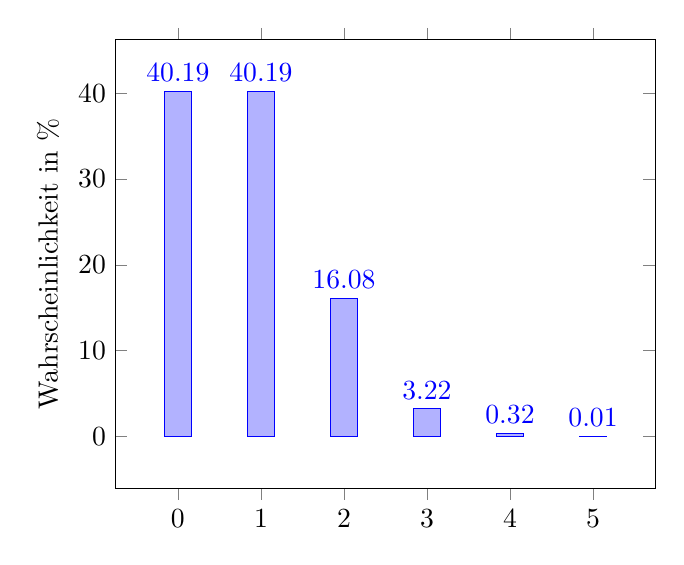
\begin{tikzpicture}
    \begin{axis}[
            ybar,
            enlargelimits=0.15,
            ylabel={Wahrscheinlichkeit in \%},
            symbolic x coords={0, 1, 2, 3, 4, 5},
            xtick=data,
            nodes near coords,
            nodes near coords align={vertical},
            /pgf/number format/fixed,
        ]
        \addplot coordinates {
                (0, 40.19)
                (1, 40.19)
                (2, 16.08)
                (3, 3.22)
                (4, 0.32)
                (5, 0.01)
            };
    \end{axis}
\end{tikzpicture}

\section{Aufgabe 2}

\subsection{a}

Sie haben Geburtstag und Ihr Lieblingsonkel liebt seltsame Geschenke. Als Teil
seines Geburtstagsgeschenks sollen Sie ein Spiel mit ihm spielen: sie müssen 10
Mal mit einem 12-seitigen Würfel würfeln. Würfeln Sie dabei mindestens 2 Mal
den Monat Ihres Geburtstags, dann schenkt Ihr Onkel Ihnen ein neues Fahrrad.
Wenn nicht, schenkt er Ihnen eine Tafel Schokolade. Wie groß ist die
Wahrscheinlichkeit dafür, dass Sie ein Fahrrad bekommen?

\begin{align*}
    X = \text{"Anzahl gewürfelter Geburtsmonate"}          \\
    X \sim B\left(n, p\right)                              \\
    X \sim B\left(10, \frac{1}{12}\right)                  \\
    P(X) = \begin{pmatrix}
               n \\ k
           \end{pmatrix} \cdot p^k \cdot {(1 - p)}^{n - k} \\
    P(X \geq 2) = 1 - \left(
    \begin{aligned}
             & \binom{10}{0} \cdot {\left(\frac{1}{12}\right)}^0 \cdot {\left(1 - \frac{1}{12}\right)}^{10-0}   \\
             & + \binom{10}{1} \cdot {\left(\frac{1}{12}\right)}^1 \cdot {\left(1 - \frac{1}{12}\right)}^{10-1}
        \end{aligned}
    \right)                                                \\
    P(X \geq 2) \approx 1 - \left(
    \begin{aligned}
             & 0.4189   \\
             & + 0.3808
        \end{aligned}
    \right)                                                \\
    P(X \geq 2) \approx 1 - 0.7997                         \\
    P(X \geq 2) \approx 0.2003                             \\
    P(X \geq 2) \approx 20.03\%
\end{align*}

\subsection{b}

In einer Pralinenschachtel sind 8 mit Marzipan und 8 mit Nougat gefüllte
Pralinen, die von außen gleich aussehen, zufällig angeordnet. Sie entnehmen und
verspeisen 5 Pralinen. Wie groß ist die Wahrscheinlichkeit dafür, dass alle 5
Pralinen mit Marzipan gefüllt sind?

\begin{align*}
    X = \text{"verspeisten pralinen mit Marzipan"}                     \\
    X \sim H\left(N, M, n\right)                                       \\
    X \sim H\left(16,  8, 5\right)                                     \\
    P(X) = \frac{\begin{pmatrix}
                         M \\ k
                     \end{pmatrix} \cdot \begin{pmatrix}
                                             N - M \\ n - k
                                         \end{pmatrix}}{\begin{pmatrix}
                                                            N \\ n
                                                        \end{pmatrix}}     \\
    P(X = 5) = \frac{\begin{pmatrix}
                             8 \\ 5
                         \end{pmatrix} \cdot \begin{pmatrix}
                                                 16 - 8 \\ 5 - 5
                                             \end{pmatrix}}{\begin{pmatrix}
                                                                16 \\ 5
                                                            \end{pmatrix}} \\
    P(X = 5) = \frac{\begin{pmatrix}
                             8 \\ 5
                         \end{pmatrix} \cdot \begin{pmatrix}
                                                 8 \\ 0
                                             \end{pmatrix}}{\begin{pmatrix}
                                                                16 \\ 5
                                                            \end{pmatrix}} \\
    P(X = 5) = \frac{56\cdot 1}{4368}                                  \\
    P(X = 5) = \frac{56}{4368}                                         \\
    P(X = 5) = \frac{1}{78}                                            \\
    P(X = 5) \approx 0.0128                                            \\
    P(X = 5) \approx 1.28\%                                            \\
\end{align*}

\subsection{c}

Erinnern Sie sich an Max aus dem PIN-Beispiel (Foliensatz zu ST-K03, Seite 2
und 3)? Angenommen, er braucht 20 Sekunden, um eine PIN zu probieren. Wie groß
ist (im Szenario von Seite 3) die Wahrscheinlichkeit dafür, dass der innerhalb
von 5 Minuten die richtige PIN errät, wenn er sich merkt, welche PINs er
bereits durchprobiert hat? Wie groß ist die Wahrscheinlichkeit, wenn er sich
nicht merkt, welche Zahlenkombinationen er bereits durchprobiert hat?


	\chapter{Übungsblatt 7}

\section{Aufgabe 1}

Herr Huber hat eine Alarmanlage in seinem Auto installiert. Es werden die Ereignisse A: "Alarmanlage springt an" und E: "Jemand versucht, das Auto aufzubrechen" betrachtet. Beschreiben Sie die folgenden bedingten Wahrscheinlichkeiten mit Worten: $P(A|E), P(E|A), P(A|E^C), P(E|A^C)$. Welche dieser bedingten Wahrscheinlichkeiten möglichst hoch bzw. niedrig seien?

\begin{itemize}
    \item $P(A|E)$ \texttt{Die Alarmanlage springt an, unter der Bedingung dass jemand versucht, das Auto aufzubrechen}: Die Wahrscheinlichkeit hierfür sollte möglichst hoch sein, da dies der sinn der Alarmanlage sein. Im idealfall sollte die Wahrscheinlichkeit hierfür gegen 100\% sein.
    \item $P(E|A)$ \texttt{Jemand versucht, in das Auto einzubrechen, unter der Bedingung, dass die Alarmanlage angeht}: Die Wahrscheinlichkeit hierfür sollte hoch sein, aber nicht 100\%, da die Alarmanlage den Dieb verschrecken sollte.
    \item $P(A|E^C)$ \texttt{Die Alarmanlage springt an, unter der Bedingung, dass niemand versucht, das Auto aufzubrechen (Fehlarlarm)}: Die Wahrscheinlichkeit hierfür sollte möglichst niedrig sein, da niemand versucht in das Auto einzubrechen.
    \item $P(E|A^C)$ \texttt{Jemand versucht, in das Auto einzubrechen, unter der Bedingung, dass die Alarmanlage \textbf{nicht} angeht}: Die Wahrscheinlichkeit hierfür sollte sehr niedrig sein.
\end{itemize}

\section{Aufgabe 2}

Bei einer Sportveranstaltung wird ein Dopingtest durchgeführt. Wenn ein Sportler gedopt hat, dann fällt der Test zu 99\% positiv aus. Hat ein Sportler aber nicht gedopt, zeigt der Test trotzdem zu 5\% ein positives Ergebnis an. Aus Erfahrung weiß man das 20\% der Sportler gedopt sind.

\begin{center}    
    \begin{forest}
    prob/.style={
        edge label={node[midway, auto, sloped, font=\small]{#1}}
    },
    for tree={
        draw,
        circle,
        minimum size=1.8em,
        l sep=1.5cm,
        s sep=1.5cm,
    }
    [
        [D, prob={$20\%$}
            [P, prob={$99\%$}]
            [$\overline{P}$, prob={$1\%$}]
        ]
        [$\overline{D}$, prob={$80\%$}
            [P, prob={$5\%$}]
            [$\overline{P}$, prob={$95\%$}]
        ]
    ]
    \end{forest}
\end{center}

\subsection{a}

Wie groß ist die Wahrscheinlichkeit dafür, dass ein Dopingtest positiv ausfällt?

\begin{align*}
    0.2 \cdot 0.99 + 0.8 \cdot 0.05 = 0.238 = 23.8\%
\end{align*}

\subsection{b}

Wie groß ist die Wahrscheinlichkeit dafür, dass der Test negativ ausfällt, obwohl der Sportler gedopt hat?

\begin{align*}
    1\%??
\end{align*}

\subsection{c}

Wie groß ist die Wahrscheinlichkeit dafür, dass ein Sportler gedopt hat, falls sein Dopingtest negativ ausgefallen ist?

\begin{align*}
    \frac{0.2 \cdot 0.01}{0.8 \cdot 0.95} = \frac{0.002}{0.76} = \frac{1}{380} \approx 0.0026 = 0.26\%
\end{align*}

\section{Aufgabe 3}

Herr Mayer kommt im Durchschnitt an 10 von 100 Tagen zu spät für den Vorlesungsbeginn zur Hochschule. Er fährt manchmal mit dem eigenen Auto zur W-HS, an 60\% aller Vorlesungstage nimmt er jedoch öffentliche Verkehrsmittel. Er hat beobachtet, dass er durchschnittlich in 5\% aller Fälle mit dem Auto unterwegs ist und zu spät zur Hochschule kommt. Sind das Zu-Spät-Kommen und die Nutzung des eigenen Autos voneinander stochastisch unabhängig?

Das Zuspät kommen ist stochastisch abhängig, da die Nutzung des Autos direkt in verbindung mit der Wahrscheinlichkeit, dass Herr Mayer zu spät kommt, steht.

\section{Aufgabe 4}

Seien $(\Omega, \mathcal{P}(\Omega), P)$ ein Wahrscheinlichkeitsraum und seinen $A, B, C \subset \Omega$ drei Ergebnisse. Man sagt, $A, B$ und $C$ seien \textit{Vollständig stochastisch unabhängig}, wenn gilt, dass

\begin{itemize}
    \item $P(A \cap B) = P(A) \cdot P(B)$
    \item $P(A \cap C) = P(A) \cdot P(C)$
    \item $P(B \cap C) = P(B) \cdot P(C)$
    \item $P(A \cap B \cap C) = P(A) \cdot P(B) \cdot P(C)$
\end{itemize}

Beantworten Sie die folgenden Fragen:

\subsection{a}

Was ist der Unterschied zwischen vollständiger stochastischer Unabhängigkeit und paarweiser stochastischer Unabhängigkeit?

Paarweise Stochastische unabhängigkeit ist gegeben, wenn die Bedingung $P(A \cap B \cap C) = P(A) \cdot P(B) \cdot P(C)$ \textit{nicht} gegeben ist, aber alle anderen Bedingungen gegeben sind.

\subsection{b}

Wie kann man diese Definition auf beliebig viele Ereignisse verallgemeinern?

\subsection{c}

Finden Sie ein Beispiel für drei Ereignisse, die paarweise stochastisch unabhängig sind, aber nicht vollständig stochastisch unabhängig.

\end{document}
